%!TEX  root=./LIVRO.tex

\chapter{\emph{Riku}}\label{riku}

\begin{figure}[H]
\centering
  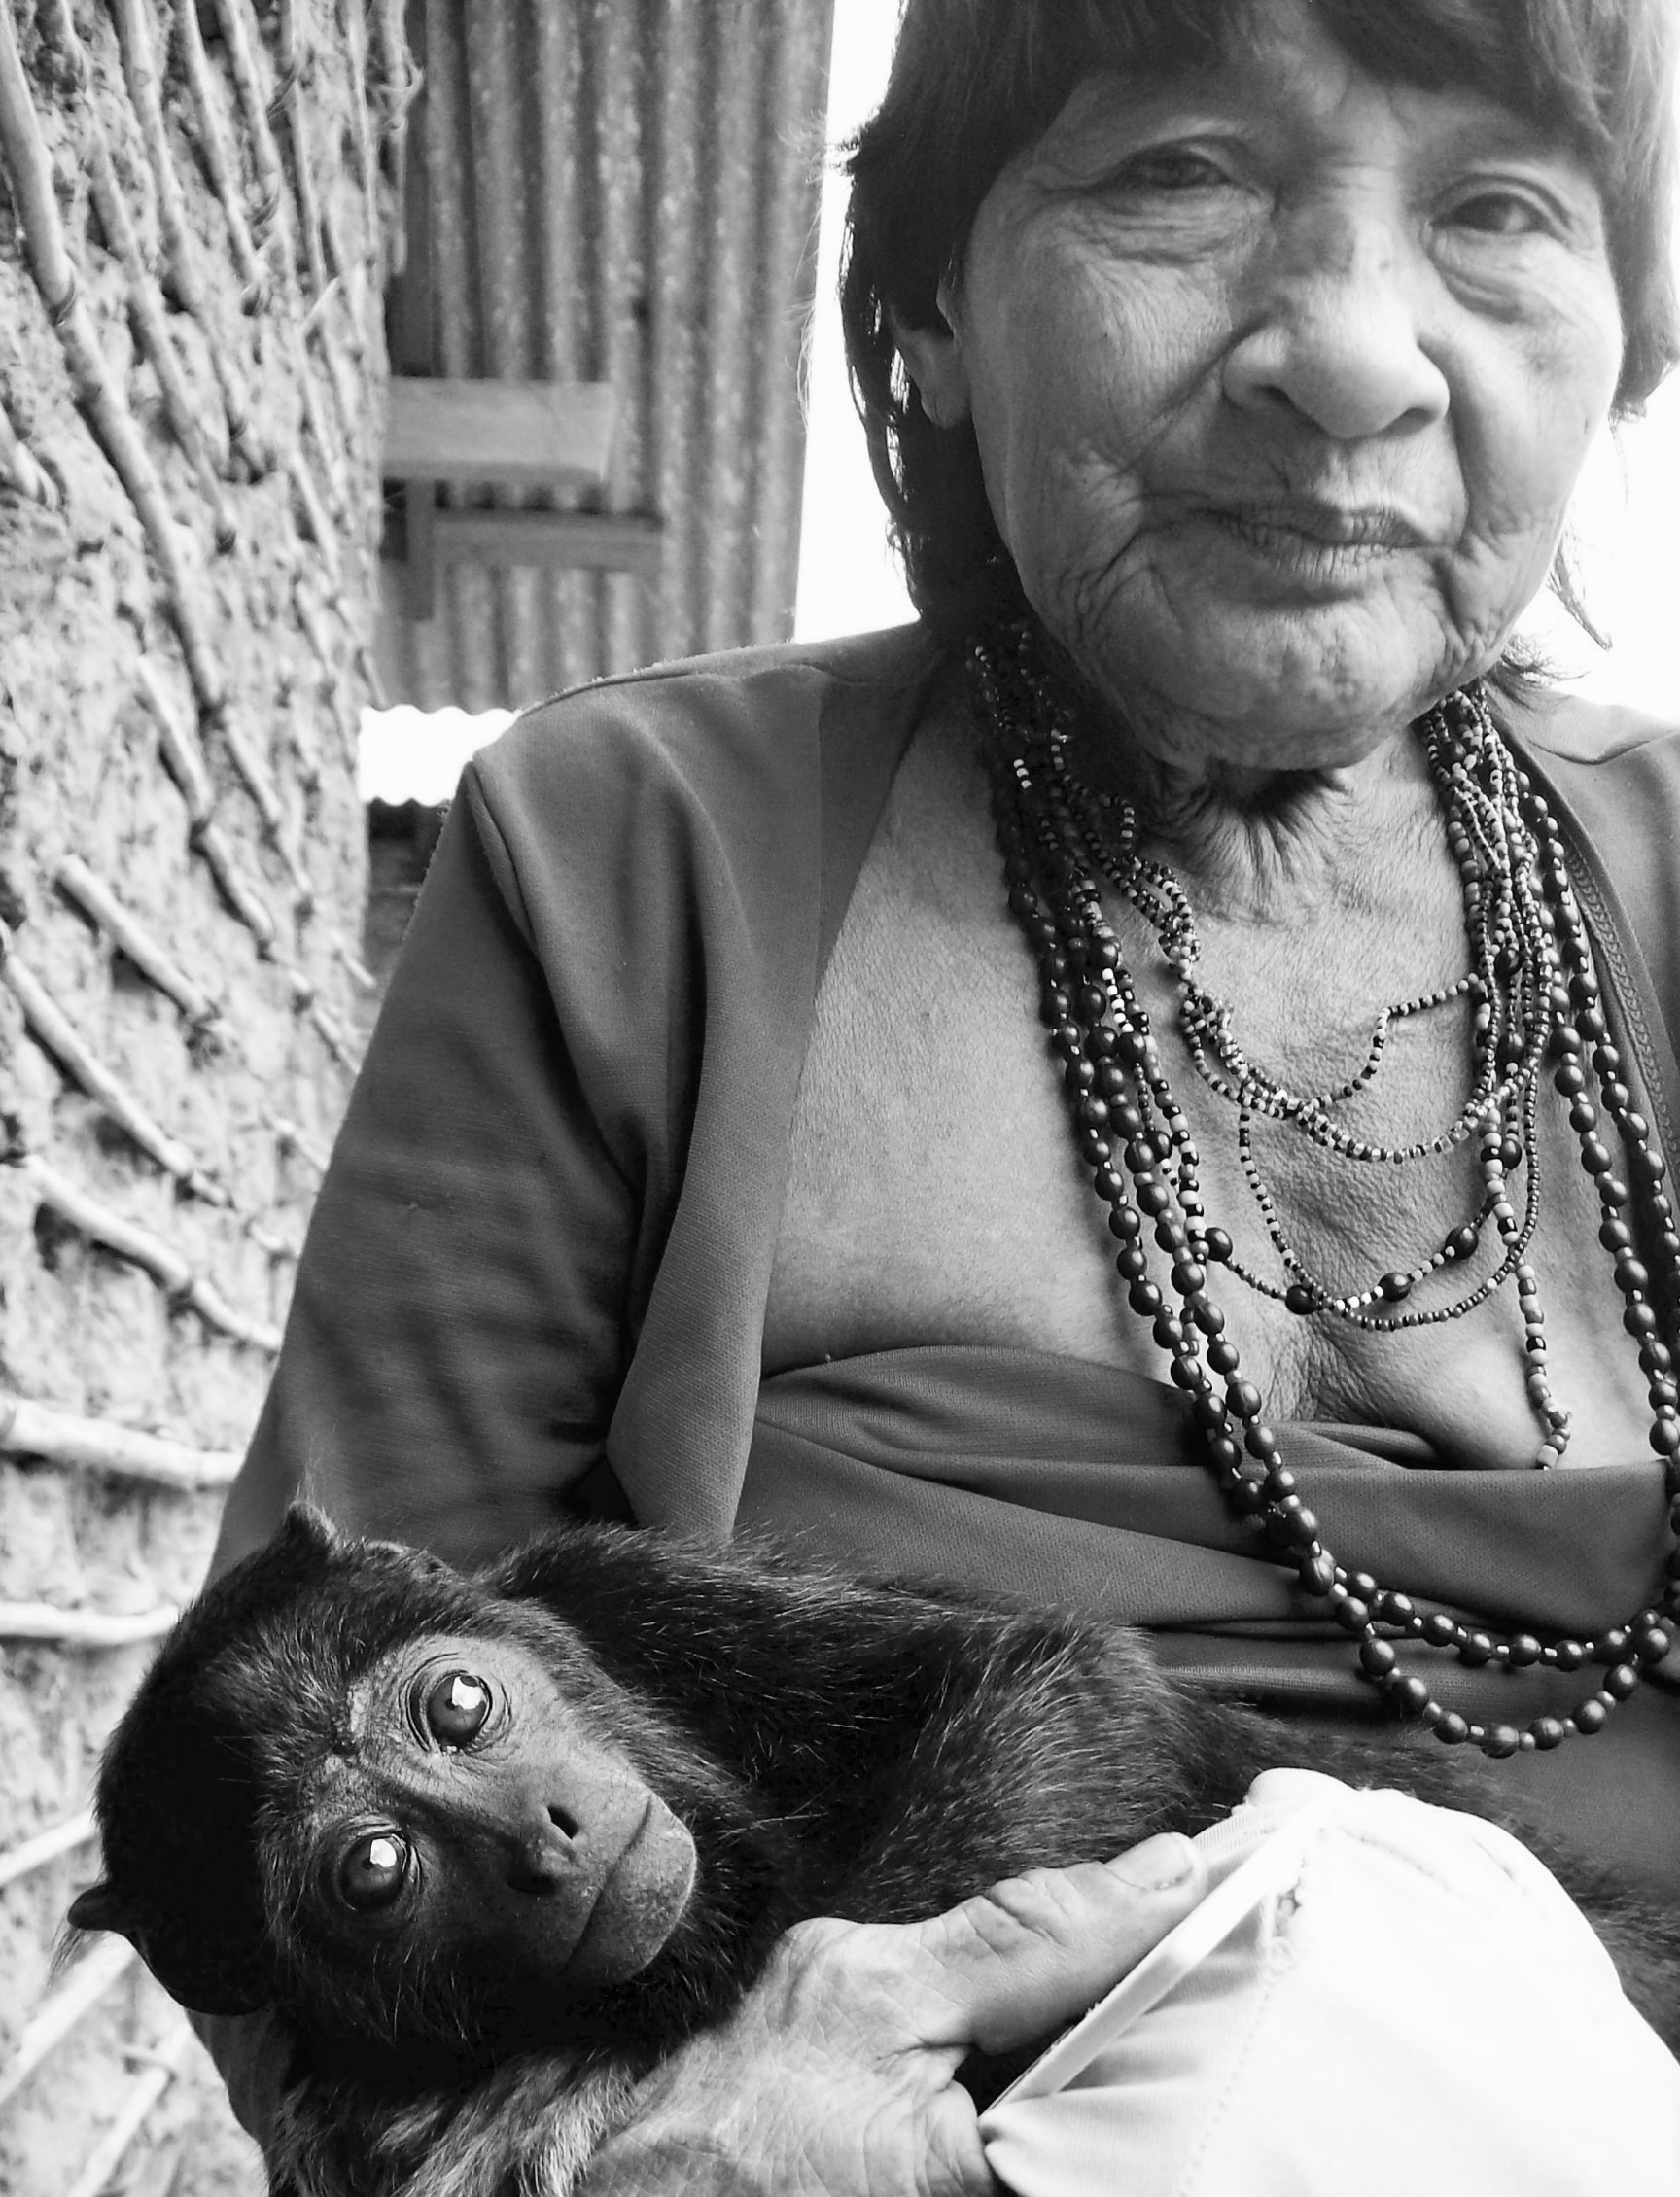
\includegraphics[width=100mm]{./imgs/100_3892}
\caption{Amy͂ Paranawãja e seu capelão de criação (aldeia Tiracambu, 2008).}
\end{figure}

\noindent O ano era 2007. Em uma manhã úmida de inverno, eu acompanhava a família
de Wirahoa em mais uma caçada. Após sairmos da aldeia, atravessamos uma
roça de mandioca, seguida de uma capoeira velha (\emph{komỹna}) que
separava a floresta (\emph{haka'a ``minha floresta''}) do espaço da
aldeia (\emph{haripa ``minha casa''}). Antes de adentrarmos a floresta,
avistei um grupo de borboletas brancas levantando voo enquanto
passávamos. Devido à beleza da cena, indaguei a meus companheiros: ``como
vocês chamam borboletas como aquelas?''. Wirahoa me respondeu que
tratavam"-se de borboletas brancas, \emph{panỹ xũa}, e emendou:
\emph{kamixa panỹ}, ``são as borboletas do jabuti''. Um pouco confuso
perguntei se era o nome da ``espécie'' de borboleta, e ele me disse que
não, que as borboletas eram \emph{kamixa nima}, em uma tradução literal,
``animais de criação dos jabutis''. Foi a primeira vez que mencionaram o
fato de um animal --- por assim dizer --- ter outro como animal de criação.
A partir de então me relataram um processo muito característico da
etologia Guajá, em que animais têm relações do tipo \emph{riku} (de
criação); alguns serão \emph{nima} (crias) ou \emph{jara} (criadores) de
outros, domesticando"-se conforme uma \emph{teoria da relacionalidade}
bastante particular.

Desta forma, muitos seres se enxergam como \emph{jara} de outros
\emph{nima}, e como tal são vistos pelas criaturas com que se
relacionam. Formigas tucandeiras são animais de criação de macacos
capelães; os porcos do mato criam algumas espécies de cobra; os poraquês
(peixes elétricos) são donos de diversas espécies de peixes e, por sua
vez, animais de criação para os jacarés (\emph{jakare} \emph{nima}
``xerimbabo do jacaré''); assim como toda espécie de mel, dentre as
dezenas existentes, pertencerá a algum ser que é seu \emph{jara}. De uma
maneira geral, muitos animais caçados pelos humanos são animais de
criação de outros animais. Em todos esses casos encontramos a mesma
relação, \emph{jara} (criador) → \emph{riku} (a relação) → \emph{nima}
(cria), em que \emph{riku} é o vetor destes polos. A proposta deste
capítulo é apresentar as muitas formas com que a relação \emph{riku}
opera no mundo Guajá. A hipótese aqui defendida é que o parentesco, tal
como discutido no capítulo anterior, é uma das formas em que a relação
\emph{riku} aparece, mas não a única. Veremos aqui como tal relação
atravessa diferentes formas de subjetividade, e dentre elas, como vimos,
está também a conjugalidade. Muito embora os Guajá não mencionem nenhum
verbo para \emph{casar}, em nossas conversas o casamento era explicado
pela ideia de \emph{riku}; a relação entre homens e mulheres que vivem
juntos. Para um \emph{awatea} (homem ou uma mulher), estar ligado a
alguém por ``casamento'' significa estabelecer com seu cônjuge uma relação
do tipo \emph{riku}.

\section{Criando seres}\label{criando-seres}

Na língua Guajá a raiz do termo para os animais de criação é \emph{ima},
podendo ocorrer associado a um nome, sob a forma \emph{nima} ``animal de
criação de'', como nos exemplos \emph{Pakwa'ĩ nima} --- ``o animal de
criação de Pakwa'ĩa'' ou \emph{Amỹ nima} --- ``o animal de criação de
mamãe''; além de poder ocorrer associado a marcas de pessoa, como no
exemplo \emph{hanima}, ``meu animal de criação''. Em meu texto oscilarei
entre a utilização das formas \emph{nima} e \emph{hanima}. A categoria
complementar a -\emph{ima} é \emph{ja}, que aparece na maior parte dos
contextos pronunciada como \emph{jára} ou \emph{jará}, a depender da
variante linguística do falante. \emph{Ja}- é cognato do -\emph{jar}
waiãpi apresentado acima, e um conhecido termo Tupi"-Guarani cuja
tradução mais conhecida é ``dono'' ou ``mestre''.

Os animais domésticos, por exemplo, quase sempre capturados na floresta,
são desses seres \emph{nima} de quem os humanos são \emph{jara}, e com
quem estabelecem uma relação do tipo \emph{riku}. O termo \emph{nima}
dificilmente poderá ser compreendido sem lançarmos mão de seu inverso,
ou complemento, que é a ideia de \emph{jara}, e ambos só serão
apreendidos se postos em relação a partir da ideia de \emph{riku}. Para
o caso Guajá, a relação existente entre um \emph{jara} e um \emph{nima}
é do tipo \emph{riku}, isto é, todo \emph{nima} será ``criado'' (segundo a
tradução Guajá) ou estará associado a um \emph{jara}. Tal relação
figurará em diversos ambientes, como a conjugalidade, caça e cosmologia.

As pessoas da aldeia Juriti não faziam um uso deliberado da ideia de
``dono'' para traduzir \emph{jara}. Ainda assim, penso que se alguma
tradução pudesse ser feita, certamente a ideia de ``dono'', tal como
aparece em outras etnografias, seria um termo aceitável. Por exemplo, em
2008, os funcionários do \versal{PIN} Juriti compraram um jumento --- na verdade,
uma jumenta --- a fim de ajudar os Guajá durante os trabalhos na roça,
principalmente para carregar os pesados fardos de mandioca e arroz.
Embora eventualmente utilizassem a jumenta como um animal de carga, o
uso que os Guajá deram ao animal não correspondia aos anseios dos
servidores do posto. Nos dias de trabalho de roça, enquanto os homens
iam e voltavam da lavoura, muitas vezes atravessando brejos, carregando
pesadas cargas de mandioca e outros cultivares, as crianças passeavam
animadamente pela capoeira com a jumenta, sem que ninguém se importasse
em colocá"-la para trabalhar --- com exceção dos funcionários do posto, que
reclamavam bastante e com frequência tentavam intervir nessa dinâmica,
mostrando o que deveria ser feito com o animal. Os Guajá, no entanto,
sempre voltavam a deixá"-la como um animal doméstico, cuja principal
função é viver como tal, livre. Entretanto, tal como os cachorros que os
ajudavam na caça por ser um \emph{karai} \emph{nima}, um animal de
criação dos \emph{karaia}, as potencialidades produtivas da jumenta eram
também aproveitadas, mas muito eventualmente. Dentre todas as pessoas, o
pequeno Takwaria, na época com nove anos de idade, era quem melhor
cuidava do animal: dava"-lhe comida; encaminhava"-o para sua choupana para
que não pegasse chuva e, caso a jumenta sumisse, o menino quase sempre
sabia do seu paradeiro. Como os adultos não dispensaram especial atenção
ao animal para cuidar e alimentá"-lo, o menino Takwaria desempenhava
essas tarefas de bom grado, e passava boa parte do tempo colocando
crianças menores no lombo da jumenta para se divertirem, ou mesmo
providenciando a cangalha para o animal carregar fardos para seus pais e
familiares. A respeito do animal, todos diziam ser ``a jumenta de
\emph{Takwaria}'', ou ``\emph{Takwari} \emph{nima}'' (animal de criação do
Takwaria). Devido a seu envolvimento com o bicho, o pequeno Takwaria era
tido por todos como \emph{jumenta} \emph{jara}. Nesse caso, \emph{jara}
pode (e deve) ser traduzido literalmente por ``dono''. Dono, não como
alguém que exerce propriedade sobre algo, mas como aquele que alimenta,
cuida e cria um ser como um \emph{nima} (``o animal de criação dele'').

A ideia de ``domesticação'', que atuaria em diversas esferas, desde os
animais de criação até a relação entre afins em potencial, de uma forma
geral, não representa novidade nas análises de diferentes grupos
amazônicos. No entanto, o que deve ser verificado é se tal ideia poderia
ser concebida conjugada com outras relações que extrapolariam a ideia de
domesticação. Explicando melhor: é possível encontrar na relação de
``domesticação'' de seres --- que percebo ser deveras atuante entre os Guajá
--- elementos que permitam pensar formas mais amplas de socialidade?
Formas que conjuguem as esferas do parentesco e da cosmologia?
Interpretar as relações entre ``senhores'' e ``seres de criação'' e suas
ideias de ``mestre/dono'' e criatura --- presentes em muitos grupos da
região --- é o ponto de partida para minha investigação. No caso Guajá, é
colocado que entre um ``dono'' e uma ``criatura'' foi estabelecida uma
relação, \emph{riku}.

Desta forma, a ideia aqui é também refletir sobre questões relativas à
figura dos donos na Amazônia, propondo, junto com o capítulo anterior,
um diálogo com um dos aspectos menos explorados do tema, que é a relação
deste com a conjugalidade. Alego que, para os Guajá, as relações
recortadas dos universos dos fenômenos tratados como ``familiarização'' e
``maestria'' são não apenas coextensivas ao campo do parentesco, como
também revelam uma concepção muito particular do que seja a relação
conjugal. Apesar de dialogar com a conhecida imagem dos ``donos de roça'',
``donos de animais'', ``das águas'' e outros correspondentes, tomo o
conceito de dono aqui como uma imagem"-guia (nos termos de Strathern,
2006, p. 208) a ser mobilizada em sua definição relacional, pensada tanto
para as relações de familiarização quanto para a conjugalidade. A
continuidade ontológica entre maestria e casamento --- cosmologia e
sociologia --- para os Guajá não remete a uma alegoria simbólica que, por
analogia, se conecta a termos conjugais humanos e não"-humanos (tal como
um xamã e suas esposas celestes; ou casamentos intraespecíficos
mitológicos). Não se trata de uma conjugalidade cosmológica, mas a
própria relação de casamento é concebida como de ``criação'' e, de muitas
maneiras, homóloga a outras relações no mundo.

\asterisc

Embora não apresente em seu trabalho referências sobre as ideias de
\emph{riku} ou \emph{jara}, Cormier dedicou sua atenção aos animais
criados nas aldeias e às relações estabelecidas entre eles e os humanos.
Seu trabalho é particularmente interessante por trazer dados de um dos
aspectos sociais mais ricos da vida Guajá, isto é, a forma quase
obsessiva com que transformam filhotes de animais selvagens em animais
de estimação. Em linha gerais, a autora argumenta como o idioma do
parentesco pode informar, em muito, o modo como as pessoas se relacionam
com esses animais, principalmente na relação entre as mulheres e os
macacos capelães (\emph{Alouatta Belzebul}), que detêm um \emph{status}
diferenciado (ver Cormier, 2003, pp. 111--128).

Cormier (\emph{op. cit.}), ao apresentar a relação que os Guajá estabelecem com
seus animais de criação (\emph{pets}), mantidos na aldeia muitas vezes
em grandes quantidades, observa, inclusive, que eles podem chegar a
ultrapassar o número de seres humanos em uma aldeia. São macacos, jacus,
quatis, jacamins, cotias, pacas, tartarugas, porcos e até filhotes de
jaguar, criados pelas mulheres, crianças e, em alguns casos, pelos
homens. Da captura à soltura dos animais, o livro apresenta bem o
fenômeno. Uma das conclusões a que a autora chega é que os \emph{hanima}
seriam uma categoria intermediária entre os Guajá e os animais e
plantas, seres da floresta. Em sua apresentação, ela afirma que o termo
\emph{hanima} é ``ambíguo'', pois aparece tanto ao se referirem aos
animais criados como, por vezes, para animais caçados (Cormier, 2003, p.
94).

Essa ``ambiguidade'' observada pela autora é, no entanto, resultado do que
considero um deslize em sua análise. O equívoco está em tratar a ideia
de -\emph{ima} (\emph{hanima}, como citado pela autora) como uma
categoria em si, fruto de uma mera relação local das mulheres com esses
animais. Mesmo as mulheres que, segundo Cormier, tornam"-se ``mães'' desses
seres não são apresentadas, em seu trabalho, por meio do termo que os
próprios Guajá utilizam para se referir às donas de um animal
(\emph{jara}). A ideia de \emph{nima}, por ser um termo relacional,
contraparte, \emph{jara}, não pode ser entendida sem esse inverso
complementar. Sendo assim, veremos que animais de caça são \emph{nima}
de outros seres, isto é, estão relacionados a outros seres (humanos ou
não humanos) da mesma forma que os animais de criação de uma aldeia
estão relacionados aos Guajá.

Como mencionei anteriormente, vejamos um pequeno inventário de espécies
animais que mantêm entre si relações do tipo \emph{riku}, em que uns são
\emph{jara} e outros, \emph{nima}.

\begin{enumerate}
\def\labelenumi{\arabic{enumi}.}
\item
  \begin{quote}
  \emph{Tal como um tipo de borboletas brancas (\emph{panỹ xũa}) estão
    associadas aos jabutis (\emph{kamixa}), um tipo de tucano chamado
    \emph{kakỹa} é animal de criação (\emph{nima}) para os macacos cuxiú
    (\emph{kwixua}). Quando cantam, esses tucanos o fazem para chamar seus
    \emph{jara}, os cuxiú}.
  \end{quote}
\item
  \begin{quote}
  \emph{O veado mateiro (\emph{arapaha}) tem a cotia (\emph{akwixia}) e uma
    outra espécie de borboleta (\emph{panã}) como ``animal de criação''
    (\emph{nima})}.
  \end{quote}
\item
  \begin{quote}
  \emph{A cotia é ``dona'' (\emph{jara}) do esquilo quatipurú (ou caxinguelê),
    chamado \emph{tamakaja}}.
  \end{quote}
\item
  \begin{quote}
  \emph{O macaco capelão, chamado \emph{waria}, é ``dono'' \emph{jara} da
    formiga tucandeira (\emph{takya}) e do macaco"-da"-noite,
    \emph{aparikya}. Segundo os Guajá, a relação entre essas duas espécies
    se dá, pois tanto o capelão quanto o macaco"-da"-noite apreciam as áreas
    das árvores mais protegidas por folhas, mais escuras e seguras,
    diferentemente de outros macacos, não tão exigentes}.
  \end{quote}
\item
  \begin{quote}
  \emph{Os porcos queixadas, \emph{xahoa}, são ``donos'' (\emph{jara}) da
    cobra surucucu, chamada \emph{arykukua}}.
  \end{quote}
\item
  \begin{quote}
  \emph{Os macacos"-prego (\emph{ka'ia}) são ``donos'' (\emph{jara}) do sagui
    \emph{atamaria} (\emph{saguinus} \emph{midas} \emph{niger})}.
  \end{quote}
\item
\begin{quote}
  \emph{Um formigão chamado \emph{tapiuhua} é dito \emph{tapi'i} \emph{nima},
    ``ser de criação da anta''}.
\end{quote}
\item
\begin{quote}
  \emph{O pássaro surucuá"-de"-barriga"-vermelha (\emph{Trogon curucui}), chamado
    \emph{arakua}, é um \emph{tatu} \emph{nima}, isto é, um ``animal de
    criação dos tatus''}.
    \end{quote}
\item
\begin{quote}
  \emph{O pássaro chora"-chuva"-preto (\emph{Monasa} \emph{nigrifons}), chamado
    \emph{jawanĩa}, é um \emph{wari} \emph{nima}, ``animal de criação''
    para um capelão}.
    \end{quote}
\item
\begin{quote}
  \emph{As cigarras \emph{jakaramuhũa} são interpretadas como \emph{hwa'ĩ}
    \emph{nima}, um ``ser de criação'' da palmeira babaçu}.
    \end{quote}
\item
\begin{quote}
  \emph{As aranhas caranguejeiras, (\emph{janũa}), são \emph{ka'i}
    \emph{nima,} ``animais de criação'' do macaco prego}.
    \end{quote}
\item
  \begin{quote}
  \emph{Os sabiás são animais de criação (\emph{nima}) das capivaras, chamadas
    \emph{kapijawara}}.
  \end{quote}
\item
  \begin{quote}
  \emph{As araracangas (\emph{ararakỹa}) são \emph{nima} dos queixadas
    (\emph{xahoa})}.
  \end{quote}
\item
  \begin{quote}
  \emph{Os esquilos quatipurus (\emph{Sciurus aestuans}), chamados
    \emph{tamakaja}, são ``animais de criação'' (\emph{nima}) dos quatis
    (\emph{kwaxia})}.
  \end{quote}
\item
\begin{quote}
  \emph{Um tipo de tatu chamado \emph{tatu} \emph{tapajnia}, por ser grande, é
    chamado \emph{tapi'i} \emph{nima} (``animal de criação das antas'')}.
    \end{quote}
\item
  \begin{quote}
  \emph{O jabuti (\emph{kamixa}) e o jabota (\emph{kamixatua}) são \emph{nima}
    para as jiboias (\emph{majhua})}.\\
  ~\\
  \emph{Nos rios ('\emph{ya}), peixes e outros seres também mantêm relações
    do tipo \emph{riku}:}
    \\
  \end{quote}
\item
  \begin{quote}
  \emph{A piaba (\emph{hipija}) é também chamada \emph{xaho pira} (``peixes do
    queixada''), pois são animais de criação dos queixadas}.
  \end{quote}
\item
  \begin{quote}
  \emph{Uma enguia chamada \emph{mahua} é um \emph{manaky} \emph{nima}, um
    animal de criação do poraquê}.
  \end{quote}
\item
  \begin{quote}
  \emph{O poraquê (\emph{manakya}), por sua vez, é ``dono'' (\emph{jara}) de
    diversos peixes de um rio}.
  \end{quote}
\item
  \begin{quote}
  \emph{O jacaré (\emph{jakarea}) é \emph{jara} da capininga
    (\emph{jaxajhua}), poraquê (\emph{manakya}), traíra
    (\emph{tara'yruhua}), dentre outros peixes}.\\
  ~\\
  \emph{Além dessas, uma infinidade de relações semelhantes são traçadas, que
    muitas vezes associam seres e elementos --- que para nós são diversos
    entre si --- como nos casos abaixo:}
    \\
  \end{quote}
\item
  \begin{quote}
  \emph{Os peixes gurijuba (\emph{hi'ijua}) são \emph{jara} de um pequena
    cobra chamada \emph{i'ĩ jumaja}}.
  \end{quote}
\item
  \begin{quote}
  \emph{Os peixes traíra (\emph{tara'yruhua}) são \emph{jara} de uma cobra
    chamada \emph{tara'yruhu maja}}.
  \end{quote}
\end{enumerate}

Em todas essas situações encontramos a mesma relação \emph{jara} →
\emph{riku} → \emph{nima}, em que \emph{riku} é o vetor desses polos.
Tal forma de relação se mostra bastante normativa, ao mesmo tempo que
aberta --- parafraseando Descola (2006, p. 138) ---, e por isso não devemos
pensar que os Guajá mantêm um inventário de todas as relações possíveis,
entre todos os seres que vivem em seu mundo; não faz sentido montarmos
um vasto quadro, com inúmeras dessas relações e possibilidades para uma
coerência total do universo. O que é colocado, muito mais do que quem é
\emph{jara}/\emph{nima} de quem, é o fato de muitos seres só existirem
na medida em que estejam estabelecidas relações como esta, isto é,
alguns seres serão ``criados'' por outros ou ao menos, e para me basear
fielmente na tradução linguística, ``estarão com'' outros.

Nos chuvosos meses de janeiro a março, os mosquitos pium (\emph{pi'ũa})
atacam com intensidade algumas aldeias, quando formam verdadeiras
nuvens. A concomitância do aparecimento dos piuns com a época do pequi
(\emph{myky'á}) é ilustrada por uma relação de continuidade
sociocosmológica entre insetos e frutos. Ambos aparecem na mesma época,
e o pequi é pensado como \emph{pi'ũ nima}, ``seres de criação dos piuns'',
e os piuns, por sua vez, seriam \emph{myky'a jara}, os ``donos do pequi''.
O agradável sabor do pequi sempre será desfrutado ao lado das
inconvenientes picadas dos piuns; foram ``misturados'' (\emph{mijamema}) e
sempre aparecerão ``juntos'' (\emph{pyry}). O maior empecilho para que tal
relação continue em curso é o desmatamento que hoje assola o oeste
maranhense. Os Guajá lembram que as chuvas são enviadas por um grupo de
\emph{karawara} (``humanos celestes'') que controla as águas e as manda
periodicamente para a floresta, pois, embora vivam historicamente de
caça e coleta, a floresta é como um lugar cultivado (como sabemos que
ocorre em outras cosmologias amazônicas, como nos Achuar e os Waiãpi).
Os \emph{karawara} não enviam chuva para as áreas desmatadas, porque
onde não existem árvores não existem frutas e não haverá animais para
delas se alimentar. Por serem também caçadores (\emph{watama'a}), estes
seres cultivam as florestas para que os animais existam e eles mesmos
possam caçá"-los na Terra. O desmatamento --- que, como sempre, traz
consequências cosmológicas gravíssimas, cataclísmicas, para os povos
ameríndios --- pode estraçalhar relações como esta, uma vez que existirá
um mundo com piuns e sem pequizeiros; com criadores (ou donos) e sem
criaturas.

Por vezes, \emph{jara} serão os animais que consomem com mais
intensidade determinados frutos. Por isso as pacas são \emph{jara} do
frutinho da árvore maria"-preta (chamados \emph{wawa'ã}). Não que animais
como cotias, veados, antas, porcos, dentre outros, não se alimentem
desses frutos, mas são as pacas as que os consomem com mais intensidade.
Eles são a ``comida da paca'' (\emph{kararuhu nimi'ũa}), ou simplesmente
``estão junto'' às pacas (\emph{kararuhu pyry}), por isso as pacas são
\emph{jara} (criadoras). O mesmo acontece com várias outras espécies
vegetais, e algumas recebem na classificação o nome do animal dono, como
``mandioca de cotias'' (\emph{akwixi tyrymỹa}), ``pequis de tucanos'' e
``comida de capelão'' (\emph{wariwa}), dentre tantas outras. Da mesma
forma, os cipós (\emph{ipoja'a}) em geral são tidos como ``criados'' pelos
macacos capelães e chamados de \emph{wari nima}, ``seres de criação dos
capelães'', justamente pelo uso frequente que esses primatas fazem deles
para se locomover.

Em certa ocasião, conversando com Pira'ima'ã, ele me informou que o
\emph{jara} da árvore angelim (\emph{jari'ia}) era um corujão branco
chamado \emph{puhupuhua.} Quando perguntei em seguida se havia
\emph{jara} para a maçaranduba (\emph{mixiranyka}), ele respondeu serem
\emph{Mai nima}, uma espécie de ``resposta padrão'', dada quando não se
``sabe'' sobre o \emph{jara} de determinado ser, uma vez que muitos
seres, direta ou indiretamente, são pensados como \emph{Ma'i
rimijapokera}, ``criaturas de \emph{Maíra}'', em uma tradução literal
``objeto da criação de \emph{Maíra}'' (Magalhães, 2010, p. 211). Só então
percebi que as questões que eu colocava soavam um tanto desconexas, pois
a pergunta que a mim, etnógrafo, passaria a fazer sentido não seria
``este ser (animal, vegetal) tem dono?'', como inicialmente eu
improvisava, fazendo uso da estrutura da língua portuguesa, porém
mesclada a palavras do léxico Guajá. Minhas questões eram entendidas de
outra forma, uma vez que a língua Guajá não adota nenhuma partícula
interrogativa que exprima a ideia de uma existência abstrata (ou
absoluta), algo como o verbo ``haver'' e ``existir'', como aparecem nas
formas interrogativas do Português, em uma pergunta do tipo ``Existem
luas em Marte?'' ou qualquer outra questão que prescreva uma existência
absoluta de algo. A partícula interrogativa \emph{mõ}, na língua Guajá ---
cuja função é introduzir perguntas de informação --- sempre aparece
seguida de sufixos marcadores de tempo, espaço e posição, cujas ideias
podem ser traduzidas --- segundo Magalhães (\emph{op. cit.}, p. 78) --- como ``para
onde'', ``de onde'', ``com que/quantos'', ``quando'', ``qual dos/das'', ``qual'', e
``cadê/onde''. No exemplo: \emph{mõ poho ta mĩpe} (``Para onde vocês vão?'')
temos \emph{mõ} como partícula interrogativa (de informação) e
\emph{mĩpe} como partícula que exprime o sentido da pergunta\footnote{Além
  de \emph{mĩ-pe} no final da frase, como no exemplo acima, a partícula
  \emph{mõ} ainda pode aparecer combinada com as partículas: \emph{mijỹ}
  -- `de onde?'; \emph{mimehẽ} -- `quando?'; \emph{mijẽ} -- `com que/
  quantos?'; \emph{minawỹ} -- `qual dos/das'; \emph{mõa} -- `qual';
  \emph{mõ} -- `cadê/onde'.}.

Embora o termo \emph{ikwẽe} possa ser traduzido por ``permanecer'',
``existir'', ``viver'', não faziam sentido minhas perguntas a respeito das
relações do tipo \emph{jara}/\emph{nima} a partir de ideias do tipo ``há''
ou ``não há'' criadores e criaturas nas diversas situações. As questões
seriam melhor compreendidas em formas como ``\emph{Mõ myky'a jara mõa}?'',
isto é, ``Qual o \emph{jara} da árvore de pequi?'' Os Guajá me ensinaram
que a pergunta certa a fazer é \emph{ma'awa jara?}, em outras palavras,
``que gente é \emph{jara}?'' (ou ``quem é o \emph{jara} {[}deste ser{]}?''),
de maneira que não há significação em perguntar se tal ser ``tem'' um
dono, pois em tese todos --- ou quase todos --- o terão. Isto posto, o
repertório de combinações é bem amplo, tanto que em diversas situações
não conseguiam saber qual era o \emph{jara} de determinado ser, embora
soubessem que um ser seria possuído.

Da mesma forma, as respostas nunca eram taxativas e, quando feitas em
português, eram sempre respondidas com um ``\emph{parece que é}''. Meus
amigos raramente respondiam a uma pergunta com ``sim'' ou ``não'', mas com
``parece ser''. Na língua Guajá a partícula epistêmica similativa
\emph{rawỹ/nawỹ}/\emph{nawyn} indica algo que se supõe verossímil, e
essas formas podem ser traduzidas como ``aparentemente'' (para o ver o
funcionamento desta partícula na língua Guajá, ver Magalhães, \emph{op. cit.},
p. 116). O melhor exemplo está na pergunta ``o que é?'', que na língua
Guajá aparece como \emph{ma'a nawỹ} e deve ser traduzida como ``o que
parece ser?'' Quando eu lhes bombardeava com perguntas, ainda que em
português, quase sempre as respostas iniciavam com um ``parece que\ldots{}''
ou, ``para mim é\ldots{}'', na forma \emph{a'e apo} (``deve ser/ parece'') com
outra partícula epistêmica que indica possibilidade (ou não certeza).
Podemos pensar também aqui que tal recurso linguístico se relaciona,
segundo Lima (1996), a certa ``noção de ponto de vista'', tal como
observado pela autora ao encontrar um recurso linguístico muito
semelhante entre os Yudjá. Segundo a autora:

\begin{quote}
\emph{Em meu trabalho de campo, uma das primeiras coisas a chamar"-me a atenção
foi a marca indelével, mas muito misteriosa, da noção de ponto de vista.
Certas frases, ditas para mim em português, como ``isso é bonito para
mim'', ``bicho virou onça para ele'', ``apareceu caça para nós quando
estávamos fazendo a canoa'', pareciam remeter exclusivamente à estrutura
gramatical de uma língua que eu não dominava, mas que transparecia no
português dos Juruna. Depois que comecei a arranhar algumas frases, as
construções que ensejavam tais traduções nunca deixaram de soar
estranhas; dentre as práticas juruna mais difíceis de assimilar eu as
destacaria, em primeiro lugar e sem hesitação. \emph{Amãna ube wï} ---
não é fácil dizer isso sem se desconcertar, desagradavelmente ou não.
Sentia"-me dizendo ``choveu para mim'', e não ``choveu onde eu estava''.
Essa maneira de relacionar à pessoa até mesmo os acontecimentos mais
independentes e alheios à nossa presença deixa sua marca na cosmologia
juruna, mas nem presumo que todas as categorias gramaticais tenham o
mesmo papel em uma cultura, nem acredito que exista a mais remota
possibilidade de algum de nós se colocar na pele de um Juruna para
captar o sentido que assumiria a vida humana em uma situação em que,
para nós, de repente, se tornaria aceitável, ou mesmo perfeitamente
justo, dizer: Chove para mim. Esse sentido diria respeito no máximo a
uma virtualidade que está em nós, virando"-nos pelo avesso (Lima, 1996,
p. 30)}.
\end{quote}

As formas Guajá, semelhantemente ao que a autora argumenta para os
``Juruna'', se apoiavam em dativos e locativos a ponto de descrições
cotidianas serem sempre acompanhadas também de um ``para ele'', que na
língua Guajá aparece sob as formas ``\emph{ipe}'', literalmente ``para
ele'', ou \emph{ihape}, ``para mim''(lit.). Em certa ocasião um homem
contava que sua canoa havia virado. Quando me relataram a conversa
disseram \emph{Kanũa jare ipe}, literalmente, ``a canoa virou para
ele''. Ou mesmo quando repetiam a fala de alguém, ela sempre era
acompanhada desse ``para ele'', como certa vez eu mencionei que a
pequena Aparana'ia já estava crescida e, ela, sem entender o meu
português, questionou sua mãe por meio de uma interessante formulação
que é muito usada: \emph{ma'a i'ĩ nipe} ?, isto é, ``o que ele disse a
você?'', e a mãe respondeu ``Ele disse que você está crescida, para
ele!''. No caso da relação \emph{riku}, estabelecida entre um
\emph{jara} e seu \emph{nima}, de maneira perspectivista ela nunca será
absoluta. Como veremos agora, um ser só estará associado (\emph{riku}) a
outro parcialmente.

Esta relação estaria no nível --- digamos --- da \emph{espécie}. São tipos
de animais que se conectam a outros dessa forma. Outros povos também
produzem categorizações entre os animais nesta chave de seres que são
``donos'' de outros. É o caso dos Karitiana, para quem os gaviões"-reais
aparecem como ``donos'' dos macacos, da maioria das espécies arborícolas
e de algumas aves, as ``caças do alto''; ao passo que a onça seria a
dona das ``caças de baixo'', como porcos do mato, veados e tamanduás
(Vander Velden, 2012, pp. 247--257). Tais ideias fazem referência aos
animais como --- digamos --- \emph{espécie} (isto é, tais espécies animais
são donas de tais espécies animais), se atualizando em relações
particulares. Por exemplo, certa vez, enquanto seguíamos os vestígios de
um bando de capelães, encontramos muito próximo ao local a que chegamos
um bando de ouriços"-cacheiros (\emph{kwanũa})\footnote{Uma espécie de
  porco"-espinho, também conhecida como ``quandú'' (\emph{Coendou
  prehensilis}).}, determinados como \emph{wari} \emph{nima} (animais de
criação dos capelães). Conseguimos abater um ou dois enquanto
lamentávamos não nos termos encontrado com os capelães. Quando indaguei
a um companheiro de caça se não estávamos, desde o início, no encalço
desses estranhos animais (os ouriços"-cacheiros), ele me explicou que as
fezes que encontramos (e seguimos) eram realmente de capelães, porém,
pelo fato de os capelães serem \emph{kwanũ} \emph{jara} (donos dos
ouriços"-cacheiros), não o admirava termos encontrado os ``xerimbabos'' no
lugar dos ``donos'', que haviam fugido. Assim, para aquele grupo
específico de ouriços, aqueles capelães (específicos) que perseguíamos
eram seus donos. Da mesma forma que, em outra ocasião, quando andávamos
na floresta seguindo alguns macacos cuxiú (\emph{kwixua}), percebemos
estar perto do bando ao ouvirmos o tucano \emph{kakỹa}, também chamados
\emph{kwixu} \emph{nima} (animais de criação dos cuxiús), voando de uma
copa de árvore à de outra. Desta forma, aqueles tucanos eram seres de
criação (\emph{nima}) do grupo de cuxiús que nós procurávamos, e não de
todos os cuxiús existentes, pois que a relação entre essa espécie de
tucano e esse tipo de primata sempre irá ocorrer.

Um animal sempre será referido pelo nome de seu \emph{jara} (seu dono)
junto com o termo \emph{nima}. Assim, como vimos, o jumento da aldeia
Juriti era chamado \emph{Takwari} \emph{nima} (animal de criação de
Takwaria); ou os macacos da mulher Panapinuhũa são chamados
\emph{Panapinuhũ} \emph{nima} (animais de criação de Panapinuhũa); e
assim por diante. Todas essas pessoas são ditas \emph{jara} de seus
animais criados, da mesma maneira que para um pai ou uma mãe pode"-se
dizer \emph{jara} de seus filhos, e animais podem ser de outros, como
acabamos de ver. Se a relação entre os animais de criação e seus donos
aparece como perfilhação, como diversos autores discutem (ver Cormier,
2003 para o caso Guajá; Erikson, 1897, 2012; Fausto, 2008), ocorre de esta
posição \emph{jara} ser concebida como própria da mãe (e por vezes do
pai) de crianças. Então, como em um ciclo infindável, se uma mulher sabe
ser dona de um xerimbabo ela o é, antes, por saber ser dona de seus
filhos, e antes disso, porque antes de filhos criou mais xerimbabos,
pois as meninas fazem isso desde crianças. Pude ver certa vez o velho
Pirama'ã pegando seu filho ainda bebê, que chorava muito, enquanto
encaminhava a criança a seu filho mais velho, dizendo: \emph{araho ja
pe}!, ``leve"-o para a dona dele'', forma sinônima de ``leve"-o para a mãe
dele''. \emph{Jara} aqui estaria muito mais próximo do \emph{iwa} Yudjá,
como \emph{aquele que possibilita a vida} de determinados seres (filhos
ou xerimbabos), do que de um ``proprietário'', já que uma das principais
tarefas de qualquer \emph{jara} é garantir o crescimento de alguém
(\emph{mixa'a}, ``crescimento dele'')\footnote{Este tema tem mobilizado
  diversos debates na antropologia do parentesco contemporânea
  encarnados na discussão em torno da ideia de \emph{nurture}, passando
  ``por análises que, incorporando fenômenos da ordem da troca e partilha
      de alimentos, de suas ressonâncias e efeitos sobre afetos e
      disposições, promovem um questionamento da barreira entre nature e
      nurture que subjaz às concepções modernas do parentesco, assim como,
      inevitavelmente, à grande parte da reflexão antropológica sobre o
      tema'' (Coelho de Souza, 2004, p. 28; ver também Battaglia, 1985; Strathern,
  1999; Carsten {[}org.{]}, 2004; para a Amazônia, ver Gow, 1997; Overing, 1999; Rival, 1998).}. A forma \emph{riku} ocorrerá entre parentes
próximos como uma maneira de produzir consubstanciação conjugal e
proximidade genealógica (Viveiros de Castro, 2002a, p. 157), bem como
também expressará formas de adoção (Fausto, 2001, pp. 413--418; Maizza, 2014,
p. 500).

Trata"-se de uma relação assimétrica, orientada, donde um \emph{nima}
sempre ``estará associado'' (\emph{riku}), ou ``será criado''
(\emph{riku}), por um \emph{jara}.

Vejamos o esquema adiante.

\begin{figure}[H]
\centering
  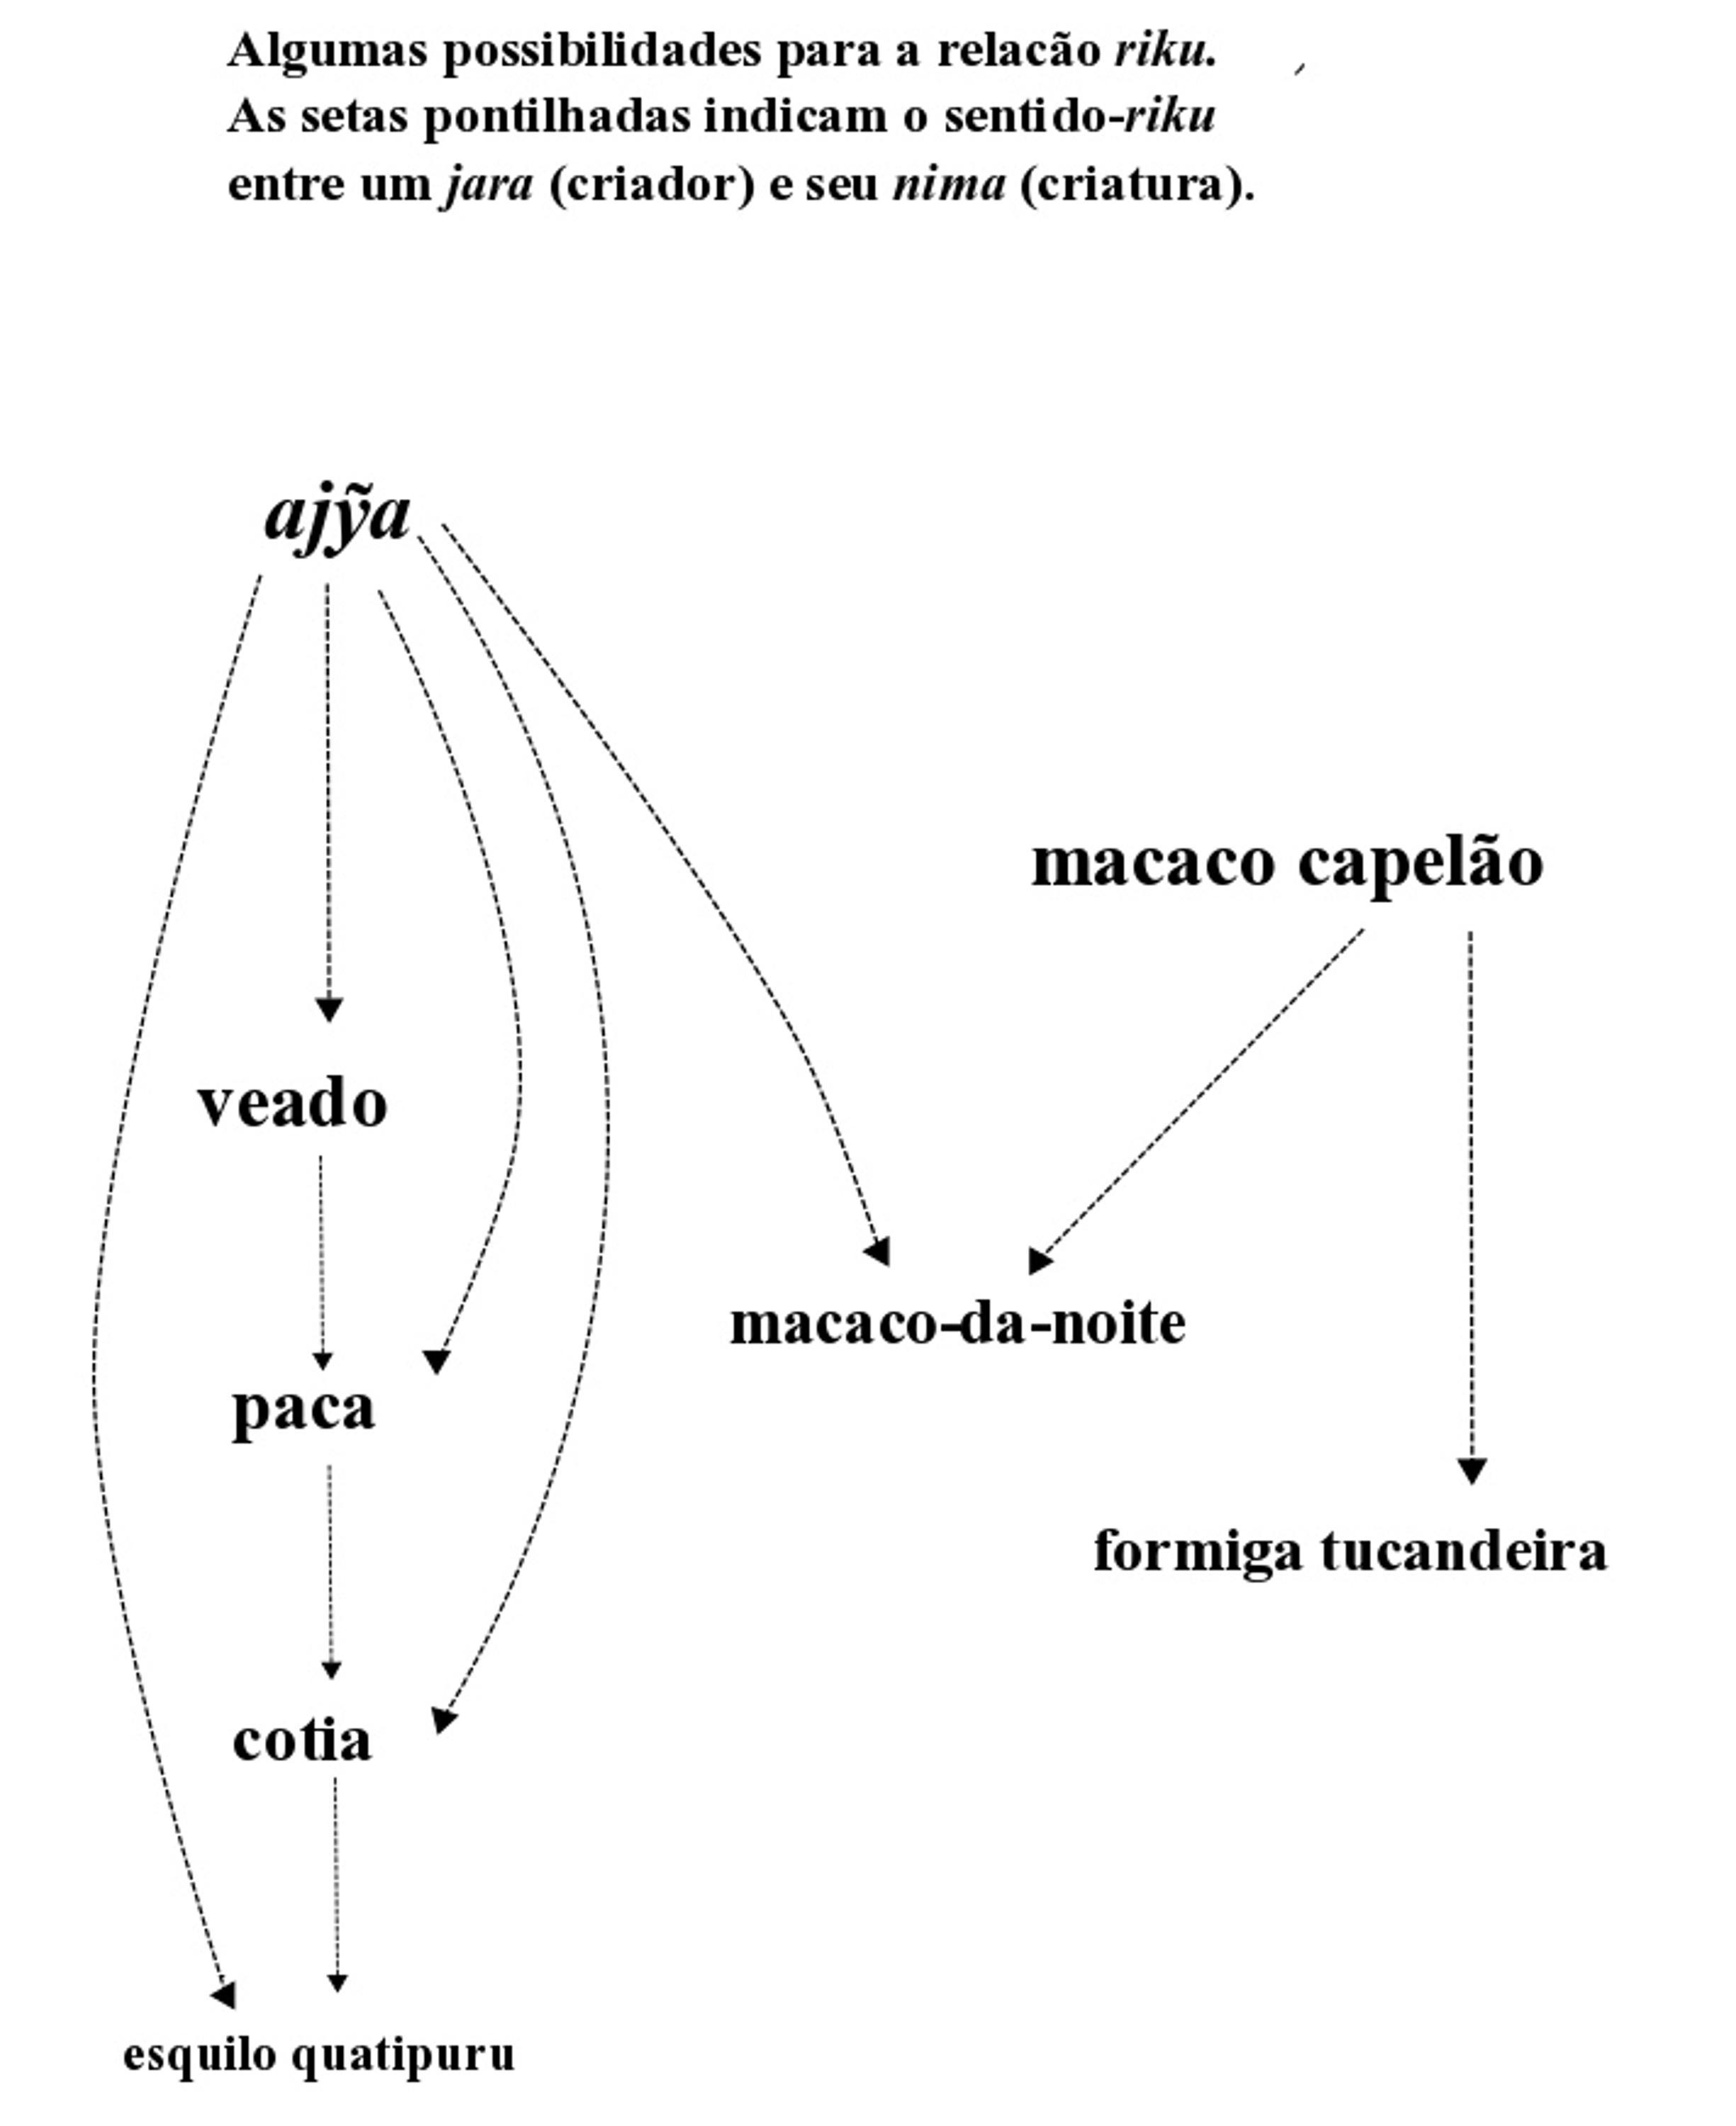
\includegraphics[width=75mm]{./imgs/Figura_11_crop}
%\caption{}
\end{figure}

%Figura 11 (10 nos originais)

A partir do quadro acima, no plano cosmológico os \emph{ajỹa} não detêm
qualquer relação de controle sobre os macacos"-capelão (\emph{waria}),
ambos pertencem, nesse caso, a universos culturais distintos. Enquanto
os animais controlados pelos \emph{ajỹa} estão, de alguma maneira,
associados aos espectros dos mortos e à ``feitiçaria'' (\emph{ma'akwa})
propiciada pelo controle dos \emph{ajỹa} sobre seus \emph{nima}
(mucuras, quatis, veados, pacas, cotias, macacos"-da"-noite), os capelães,
apesar de também deter capacidades agentivas, sobretudo na forma da
vingança pós"-caça (como veremos no capítulo 8), fazem parte de um grupo
de animais desejáveis ao consumo em qualquer época e situação\footnote{Mesmo
  na couvade pós"-parto ou reclusão por homicídio que um homem venha a
  experimentar, a carne de capelão --- junto com a farinha de mandioca e
  alguns peixes pequenos --- é a primeira a entrar na dieta tão logo o
  processo se inicie.}. Entrementes, como observamos na figura anterior,
os Guajá afirmam que tanto os \emph{ajỹa} quanto os capelães enxergam os
macacos"-da"-noite como animais de criação, da mesma forma que duas
mulheres diferentes podem manter cotias diferentes como animais de
criação. Parece não se tratar, portanto, de relações do tipo \emph{donos
da espécie} como se os \emph{ajỹa} ou capelães fossem ``os donos'' dos
macacos"-da"-noite --- um ou mais seres controlando um conjunto homogêneo de
outros seres --- embora, como veremos, também exista tal relação, ainda
que de uma forma menos intensa. Porém, no âmbito geral, a relação
\emph{riku} sugere a ideia de dono \emph{de um} espécime, e não dono
\emph{da} espécie. Um ser sempre será \emph{jara} para si e para um
outro (ou alguns outros). E a relação existente entre um \emph{jara} e
seu \emph{nima} não é incondicional, pois um \emph{jara}, para alguém,
pode ser um \emph{nima} em outra perspectiva; e isso parece estar
acordado entre os diversos seres no mundo: todos parecem saber que
alguém só será um dono \emph{a} \emph{posteriori}, isto é, uma vez
estabelecida uma relação. Se para muitos povos amazônicos a humanidade é
uma qualidade que só pode ser descrita a partir de um ponto de vista (do
corpo ou da aldeia, por exemplo), tal como Lima (1996) relata para os
Yudjá, para os \emph{awatea}, a relação \emph{riku} --- uma das melhores
possibilidades de realização de uma relação humana --- também só poderá se
desenrolar sob um ponto de vista particular.

Os macacos"-da"-noite podem ser \emph{nima} tanto dos \emph{ajỹa} quanto
dos capelães. Essas são possibilidades balizadas por relações reais que
os Guajá dizem haver entre diferentes seres; e, portanto (ainda segundo
o quadro acima), a formiga tucandeira (\emph{tahya}) é apenas um
\emph{wari} \emph{nima} (``um \emph{nima} para um capelão''); ao passo que
veado, paca e cotia --- cada um deles --- são \emph{ajỹa} \emph{nima}
(``animais de criação para os \emph{ajỹa}''). No entanto, se os
\emph{ajỹa} ``criam'' esses animais, algumas espécies também são dotadas
de um \emph{ponto de vista} que os habilita serem \emph{jara} de outros
seres. Se tomarmos como exemplos a paca (\emph{kararuhua}), o veado
(\emph{arapaha}), a cotia (\emph{akwixia}) e o quatipuru
(\emph{tamakaja}) --- animais que estabelecem uma relação do tipo
\emph{riku} entre si --- podemos ver algo assim:

\begin{quote}
\emph{1 - os \emph{ajỹa} têm como animais de criação pacas, veados, cotias e
quatipurus;}

\noindent\emph{2 - para os veados, as pacas são os animais de criação;}

\noindent\emph{3 - para as pacas, os veados são os donos (\emph{jara}), e as cotias,
animais de criação;}

\noindent\emph{4 - para as cotias, as pacas são donas (\emph{jara}), e os quatipurus,
animais de criação;}

\noindent\emph{5 - os quatipurus são somente \emph{akuxi} \emph{nima} (``animais de
criação das cotias''), não ``criam'' algum outro ser}.
\end{quote}

\begin{figure}[H]
\centering
  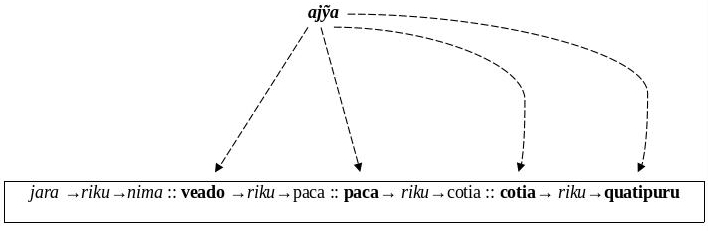
\includegraphics[width=\textwidth]{./imgs/Figura_13}
%\caption{}
\end{figure}

%Figura 11

Em paralelo, veados, pacas e cotias, mesmo sendo animais de criação dos
\emph{ajỹa,} mantêm entre si relações de consubstancialidade do tipo
\emph{hapihiara} (parentes próximos). A partir do esquema acima, tendo
como exemplo o veado, este ser é \emph{jara} para uma paca, ao mesmo
tempo que um \emph{ajỹa} será seu \emph{jara}, mantendo relações do tipo
\emph{riku}: uma paca é, para ela mesma, dona (\emph{jara}) de uma
cotia, e animal de criação (\emph{nima}) para um veado. Apesar de
estarem, por assim dizer, na ``área de influência'' dos espectros canibais
\emph{ajỹa}, esses animais são concebidos a partir de uma linha de
continuidade que coloca uns como criadores de outros. Isto não é
meramente um discurso abstrato sobre o mundo, mas implica diretamente a
vida das pessoas, sobretudo no que concerne à caça. O \emph{riku} opera
como um \emph{princípio sociológico} que mobiliza relações entre esses
seres sem necessariamente passar pela perspectiva humana. Os Guajá
apenas \emph{concebem} \emph{como os animais concebem} tais relações. Se
determinadas borboletas são seres de criação dos jabutis, ou se os
cuxiús"-pretos o são de macacos"-prego, é algo atuante entre tais seres e
escapa ao controle humano. Também não se trata de relações dentro de
relações, mas sim de uma multiplicidade delas, formando"-se muito mais
uma pluralidade de \emph{conexões parciais} do que um ``todo'', em que,
supostamente, se encapsulam partes que contenham o todo: trata"-se de
\emph{the view from a body rather than the view from above} (Strathern,
2004, p. 32)\emph{.}

Uma possibilidade para interpretar o problema, tal como os Guajá o
formulam --- como podemos ver no exemplo acima ---, é dada por Lima em um
exercício dialógico com um homem Yudjá (Lima, 2005, p. 338). Em seu pequeno
diálogo, a autora chega a uma interessante conclusão acerca da relação
entre os humanos e os \emph{'ï'anay} (os espíritos dos mortos). Assim,
há seres que se veem como sujeitos e enxergam outros seres como ``outros''
(mortos, xerimbabos, deuses), sempre do ponto de vista desse sujeito:

\begin{quote}
\emph{são três as tomadas em jogo: sua irrealidade para outrem; sua
indubitável existência para si; por fim, a realidade acima de qualquer
suspeita daquele que fala. Se as duas primeiras revelam"-se simétricas, a
terceira contém ambas: é ela a assimetria perspectiva, e ela é humana
(\emph{idem})}.
\end{quote}

Em seguida a autora reforça que a tal ``assimetria perspectiva'' pode ser
revertida também em benefício dos \emph{'ï'anay}. A partir disso, se
tomarmos o esquema acima dos \emph{ajỹa} e seus \emph{nima}, em que
esses seres criam (\emph{riku}) um conjunto de animais que mantêm também
relações particulares entre si, podemos pensar que ali atua uma
perspectiva do tipo assimétrica para os \emph{ajỹa}, o que habilitaria
tais seres a serem \emph{jara} de um conjunto de outros seres cuja
realidade da relação \emph{riku} só existiria para si mesmos. Nesse
sentido penso que os \emph{ajỹa} sejam \emph{jara} diferentes do que uma
paca é para uma cotia, simplesmente por se colocarem em relação a um
conjunto maior de seres, tal como os humanos (\emph{awatea}), ou
\emph{Maíra,} conseguem fazer.

Trata"-se menos de pensar um todo dividido entre, de um lado, donos e, de
outro, seres criados por estes, do que pensar o sistema como uma
multiplicidade de \emph{jara} e \emph{nima}, variando de acordo com as
relações estabelecidas entre os seres --- uma linguagem que concebe
múltiplos pontos de vista, com ênfase no aspecto relacional que aqui
aparece intensamente. A existência dos seres enquanto sujeitos --- a sua
consciência mesma enquanto ser vivente em oposição a outras formas de
vida --- de muitas maneiras está relacionada à possibilidade do
estabelecimento de uma relação do tipo \emph{riku}. É um problema de
posição, do tipo ``isto é dono para mim, enquanto aquilo é xerimbabo
para mim (ou para ele)''. A não totalização dessas relações em
formas"-donos do tipo ``donos da caça'', ``donos das águas'', ``donos das
roças'' --- dentre outros que aparecem à exaustão nas etnografias (para um
balanço, ver Fausto, 2008) --- é a marca de como os Guajá pensam tal
relação \emph{riku}, que nesse caso está mais próxima de uma
antimaestria (ao invés de maestria, como propõe Fausto {[}2008{]} para
ideias análogas), uma vez que mestres de criaturas, tal como outras
ontologias prescrevem (algo como propiciadores absolutos), aparecem de
maneira muito fraca aqui. Parafraseando Viveiros de Castro, não estou
com isso advogando que fujamos da noção de dono, ``como se fosse uma
categoria visceralmente antiamazônica'', mas apenas cuidando para não
confundir totalmente o que os Guajá defendem, com o que já foi defendido
para outros povos amazônicos até agora. A relação \emph{riku}
estabelecida entre um \emph{jara} e um \emph{nima}, embora proponha uma
assimetria relacional, não deve ser reduzida à ideia de ``controle'', como
continuaremos vendo.

\asterisc

Kelly, ao pôr em relação alguns regimes de socialidade amazônicos,
lembra que nas ontologias perspectivistas ``pessoas são esses seres duais
sujeito/objeto a que se creditam perspectiva e agência (participam da
cultura e têm uma alma imortal), mas que ao mesmo tempo são objeto de
outra subjetividade (parte da natureza de alguém)''. As posições eu/outro
de coletivos como esses --- seja em relação aos humanos, animais ou
espíritos --- vão variar de acordo com o ponto de vista de quem quer que
esteja se relacionando:

\begin{quote}
\emph{Pessoas, portanto, não são nem objeto nem sujeito, mas ambos: o ponto
 de encontro de um Eu reflexivo e da perspectiva do Outro. O contexto
 determinará quanto a qualidade"-de"-sujeito (\emph{subjectness}) ou a
 qualidade"-de"-objeto (\emph{objectness}) será prevalecente em uma
 relação. (\ldots{}) A consciência de uma pessoa de sua
dualidade sujeito"-Eu/objeto"-Outro expressa"-se, principalmente, no seu
reconhecimento da possibilidade de se tornar presa de alguém (Kelly, 2001, p. 100)}.
\end{quote}

No caso Guajá (e parafraseando Kelly), a consciência de uma pessoa sobre
sua dualidade eu/outro expressa"-se, principalmente, no reconhecimento de
tornar"-se \emph{nima} ou \emph{jara} para alguém, isto é, na
possibilidade da instauração de uma relação do tipo \emph{riku}. Pensar
a \emph{relação para} não é torná"-la menos real, ou menos resistente,
como se o fato de estar baseada em pontos de vistas obscurecesse as
relações reais no mundo: ``um ponto de vista não é uma opinião subjetiva''
(Viveiros de Castro, 2002, p. 386). Assim, não há nada de subjetivo no
fato de um ouriço"-cacheiro ser um \emph{nima} para um macaco"-capelão, ou
um poraquê ser um \emph{jara} para a traíra. Se observarmos tais
proposições sem nos basear na ideia de Natureza, como algo que organiza
``naturalmente'' o mundo, e nos abalizarmos por esse outro sistema de
pensamento, em que o efeito de boa parte das relações entre seres e
coisas (que a nossa ontologia defende serem ``fatos'' da Natureza ---
apesar de os fatos serem feitos, diria Bachelard {[}Latour, 1994,
p. 24{]}) produz outro tipo de autonomia, conseguiremos nos aproximar do
mundo Guajá e, consequentemente, pensar ``alguma antropologia'' em cima
desses fatos (que não são mais da Cultura nem da Natureza). Voltemos
mais diretamente à etnografia para observarmos pequenos exemplos que
podem explicitar meus argumentos.

\subsection{Exemplo 1 --- Pragas}

\forceindent
Uma aldeia Guajá não é local dos mais confortáveis, e quem afirma isso
são eles --- os Guajá --- mesmos\footnote{O contraste entre aldeia e mata e
  entre aldeia e céu é ressaltado todo o tempo pelas pessoas.}.
Acostumados ao frescor e à liberdade da floresta, onde permaneceram
vivendo até o recente contato, a aldeia, que veio como parte do ``kit
pacificação'' (refiro"-me à agricultura; utensílios e espingarda), ainda
é algo novo para todos. A aldeia é um local \emph{manahỹ} (feio),
enquanto a floresta seria \emph{parahỹ} (bonito). Parafraseando Viveiros
de Castro quando escreve sobre a aldeia Araweté, o que ocorre com os
Guajá são aldeias junto a Postos Indígenas, e não o contrário; e a
aldeia é muitas vezes chamada de ``\emph{Funai}'' pelas pessoas. Os
tapiris (\emph{tapãja}) cederam lugar às casas de taipa. E a
concentração de pessoas em uma única aldeia trouxe, além das galinhas e
cachorros, muitas baratas. O amontoado de coisas e comida que os Guajá
estocam em seus telhados de palha e brechas de parede é tamanho que
todas as noites uma miríade de baratas aparece zanzando em boa parte dos
espaços das casas, do chão ao teto. Nas noites úmidas de inverno, sobem
por nossas pernas circulando por todo o corpo, por dentro e por fora da
roupa, da cabeça aos pés. A quantidade de baratas é tão grande que eu
(particularmente) tive de me acostumar aos movimentos delas por meus
braços e pernas. Quando espantávamos uma do braço, duas já estavam no
tornozelo.

Certa vez, conversando sobre o desconforto que as baratas traziam à
aldeia, Wirahoa me disse que elas eram de responsabilidade da antiga
\versal{SUCAM}\footnote{Superintendências de Campanhas de Saúde Pública, antigo
  órgão da Fundação Nacional de Saúde (Funasa), que por sua vez deu
  lugar à a \versal{SESAI} (Secretaria Especial de Saúde Indígena).}. E disse
mais: que as baratas eram \emph{sucam nima}, isto é, ``animais de
criação da \versal{SUCAM}'' (criaturas cuja vida e o controle da vida é
propiciado pela \versal{SUCAM}). Em linhas gerais, a \versal{SUCAM} é \emph{jara} das
baratas. Segundo Wirahoa, ``a \versal{FUNAI} foi a responsável por trazer as
baratas até a aldeia'', porém, por não ser um \emph{jara} das baratas, a
\versal{FUNAI} teve que chamar o verdadeiro ``dono'' delas, a \versal{SUCAM}, ela sim, por
ser o \emph{jara} verdadeiro (\emph{jaretea}) saberia controlar essa
praga. Cada vez que um funcionário da \versal{SUCAM} vai até a aldeia, ele não
está indo para exterminar as baratas, mas sim para controlá"-las, pois
elas são as suas ``criaturas''. Um não vive sem o outro. É disso que se
trata o \emph{riku}. É esta a relação entre a \versal{SUCAM} e as baratas, uma
relação de \emph{criação}.

Ainda dentro da categoria ``pragas'', assim como a \versal{SUCAM} é \emph{jara}
das baratas, um cachorro pode ser \emph{jara} de suas pulgas, tal como
uma anta de seus carrapatos (\emph{jatikoa}). Quando abatem animais
grandes como porcos, veados e principalmente antas, os Guajá, maldizendo
o animal, queimam com um ramo seco de palhas os pelos do bicho, a fim de
tirar todos os carrapatos. E reclamam das antas por ``gostarem'' de criar
tantos carrapatos. Dizem: ``\emph{tapi'ira} \emph{jatikoa riku}'' (``A
anta cria {[}\emph{riku}{]} carrapatos''). As mordidas de carrapato, que
qualquer um de nós adquire nas caminhadas pela mata, são associadas a um
animal específico: ``Esses são os carrapatos de um veado que passou por
aqui'', ou ``eu fui mordido pelo carrapato daquele porco, ou daquela
anta''. Cada carrapato também tem o seu \emph{jara}. Não que nesses
casos as antas, porcos e veados controlem os carrapatos, mas,
diferentemente disso, os carrapatos apenas ``estão com'' esses animais já
que, como vimos acima, esta é uma tradução para \emph{riku}.

Para que não haja mal"-entendido, os carrapatos são uma chateação para
todos, tal como as baratas e algumas espécies de cobra o são. E, se
dependesse das pessoas da aldeia Juriti, elas manteriam esses bichos
(todos) longe, não muito diferente do que nós mesmos pensamos e fazemos.
Porém, quando os Guajá dizem que os carrapatos e baratas só vivem a
partir destes \emph{jaras}, diferentemente de nós, estão enfatizando que
o que nós chamamos ``praga'' trata"-se de um descontrole de outra ordem,
de uma ordem fenomenológica, relacional --- da própria relação \emph{riku}
---, e não de um desequilíbrio ambiental. ``Estar com'', ``estar associado
a'', também são formas de se interpretar a relação \emph{jara"-nima} que,
se aparece como controle, como no caso das baratas, está ausente no caso
dos carrapatos.

\subsection{Exemplo 2 --- donos de nome (2ª parte)}

\forceindent
Cormier (2003, p. 91) observa que cada pessoa é designada por um nome de
planta, animal ou objeto epônimo, considerado para a pessoa o seu, nas
palavras da autora, \emph{haĩma}, ``ser de criação dele'' (um
\emph{harypihara} --- na notação da autora ---, ``consanguíneo''), havendo
assim entre a pessoa e o objeto nominador uma ``conexão espiritual''
(\emph{sic}). Ela dá como exemplo um homem chamado
\emph{takamỹxa'a}\footnote{Mesmo sendo uma citação desta autora, cito os
  nomes próprios a partir da grafia que adotei neste livro.}, que tem
como seu \emph{haĩma} a palmeira tucumã (\emph{takamỹa}). Segundo
Cormier, quando uma criança nasce ela não recebe nome algum; cabe ao pai
(ou marido da mãe), após alguns meses, ``discernir o nome descobrindo
qual forma de vida ou característica do ambiente é o \emph{haĩma} da
criança'' (Cormier, \emph{op. cit.}, p. 91). Assim argumenta a autora sobre esse
fenômeno:

\begin{quote}
\emph{Em alguns aspectos, as relações \emph{haĩma} se assemelham a um
totemismo individual. Indivíduos são considerados possuírem uma conexão
espiritual com a comunidade de outros. No entanto, não existem tabus em
se comer um membro de uma dessas comunidades de \emph{haĩma}, e
geralmente, podem ser alimentos que os Guajá comem, alimentos que não
comem, ou objetos que não sejam alimentos. Dos \emph{haĩma}
determinados, 64\% eram espíritos animais, 19\% espíritos de plantas,
6\% espíritos de aspectos ambientais, 6\% eram espíritos de bens
manufaturados, 2\% eram espíritos de mel, e 2\% espíritos de divindades.
Embora os \emph{haĩma} fossem tipicamente representados por espécies
úteis, eles não representavam necessariamente as espécies mais
utilizadas. Das espécies animais, 43\% eram espíritos de pássaros, 31\%
de espíritos de peixe, 10\% espíritos de plantas, 8\% espíritos de
mamíferos, e 8\% de espíritos de répteis (\emph{idem}, livre tradução, meus
grifos)}.
\end{quote}

A autora segue em sua análise com a suspeita de tal ``fenômeno'' ser
relacionado historicamente ao xamanismo amazônico, embora entre os Guajá
(continua ela) não exista o ``papel'' do xamã e todos os indivíduos tenham
uma germanidade do tipo \emph{haĩma} (\emph{haĩma} \emph{siblingship}).
Em seguida, Cormier conclui que tais relações têm menos a ver com o
``totemismo'' aludido anteriormente do que com a ideia de ``animismo''
(Cormier, \emph{op. cit.}, pp. 91--92).

Embora Cormier apresente dados importantes, permitam"-me fazer um
contraponto à interpretação ``animista'' e ``espiritual'' (dois termos
utilizados por ela). Além de eu não ter encontrado nenhuma relação entre
uma ideia de espírito e os nomes das pessoas, a ideia trazida por ela
(de ``conexão espiritual'') parece ser nada mais do que relações do tipo
que vimos até agora. Em outras palavras, os Guajá não mencionam nenhuma
ideia que me pareça possível traduzir como ``conexão espiritual'', porém
mencionam outras ``conexões'', por exemplo, se assim quisermos chamar a
relação \emph{riku}. As ``relações \emph{haĩma}'', aludidas pela autora
(entre um sujeito e seu nome, ou uma mulher e seu xerimbabo, dentre
outras), podem ser pensadas como aquela existente entre um ser (um
\emph{jara}) e um \emph{nima}. Se vincularmos o ``\emph{haĩma}'' ---
descrito por Cormier --- às ideias de \emph{riku} e \emph{jara} (ambas
ausentes em sua análise), poderemos propor uma alternativa à ideia de
\emph{conexão espiritual}, pensando o problema a partir de outros
regimes de afeto, como venho argumentando até aqui.

Lembro que é uma relação entre cognatos a que ocorre entre um
\emph{jara} e um \emph{nima}, e o trabalho de Cormier é rico em mostrar
como o processo de perfilhação das mulheres Guajá e seus animais criados
é traduzido como um processo de consanguinização --- outra tradução
possível para \emph{harapihiara} (como vimos no capítulo anterior). Como
um exemplo, podemos traduzir o nome \emph{Pinawãxa'a} como ``parente da
bacaba'': Pinawã (bacaba) + \emph{xa'a} (sufixo nominal e termo de
cognação que exprime proximidade genealógica e/ou consanguinidade).
Neste caso, tal como observado por Cormier, a bacaba seria uma espécie
de \emph{nima} deste homem, que pode ser visto como o seu \emph{jara}.
Assim como um homem cujo nome é \emph{Wirahoa} (Gavião) tem o gavião
como seu \emph{duplo} animal. Há, portanto, uma relação de proximidade
entre o indivíduo e o ser/coisa que o nomina e também --- como bem
observou Cormier e vimos no capítulo 3 --- uma espécie de evitação. A
possibilidade de relacionar pessoas e coisas é a tônica da onomástica
Guajá. \emph{Jara} (o nominado) e \emph{nima} (o ser ou fenômeno que
nomina) são aqui não ``donos'' e ``criaturas'' que impliquem controle, mas
seres que simplesmente estão relacionados (\emph{riku}) um com o outro e
se concebem ``juntos'' (\emph{pyry}).

Algo parecido ocorre entre os Waiãpi, cujo sistema de nomes faz uma
distinção entre os que são ``só nomes'' e os que significam alguma relação
ou semelhança com um elemento da natureza --- escolhidos com o propósito
de marcar a criança no nascimento, protegê"-la de possíveis ataques dos
espíritos \emph{jurupari} e que, à medida que a pessoa cresce até se
tornar adulto, vão sendo cada vez menos pronunciados. Segundo Gallois:

\begin{quote}
\emph{para proteger uma criança, deve"-se dizer"-lhe o nome humano, para evitar
que ela seja considerada como uma criança sem dono, prestes a ser
raptada pelos seres sobrenaturais. Para proteger uma pessoa adulta,
evita"-se pronunciar seu nome justamente porque, nessa idade, os
indivíduos já acumularam uma série de relações --- de conflito ou
cooperação --- com essas entidades. Identificar a pessoa pelo nome seria
chamar a atenção sobre ela (\ldots{}) (Gallois, 180--181)}.
\end{quote}

Mesmo com a contiguidade entre nominados e seres nominadores, não é
desejável pôr em relação o nome de alguém com o ser ou o fenômeno que o
nomina (o \emph{nima}). Desta forma, alguém que se chame \emph{Kaawi'ia}
(``marimbondo''), embora seja um \emph{kaa} \emph{jara}, e que tenha
relação de proximidade com os marimbondos (\emph{kaa}) não deve ser
referido ordinariamente como um marimbondo qualquer. Em um conjunto de
etiquetas muito particulares, a onomástica Guajá relaciona pessoas e
seres, sem que uma relação real (ou seja, com seres reais) tenha que ser
mencionada. Ao contrário, a menção a esta relação pode ser vista como
uma ofensa. Pude sentir isso quando deram"-me o nome de \emph{Iramuxa'a}
(como um nome de brincadeira), cuja tradução pode ser ``parente do
inhambu''. Recebi tal nome devido às minhas longas passadas, quando
caminhávamos pela floresta, fortemente contrastada com os passos firmes
e curtos de meus amigos. Certa vez, ao avistar um inhambu aludi ser ele
uma espécie de \emph{haxa'a} (``meu parente'') para mim, ao que me
explicaram não ser aquele o meu \emph{nima} mas um outro (\emph{amõa}).
E era assim com todos os nomes, como se existisse um ser ``ideal'' (na
falta de termo melhor), de outra ordem (ainda que terreno), que nomeasse
cada um.

\subsection{Exemplo 3 --- Donos, duplos}

\forceindent
Não seria somente no plano terrestre que seres de diferentes ordens
poderiam estabelecer relações do tipo \emph{jara}-\emph{nima}. Entre a
Terra (\emph{wya}) e os patamares celestes (\emph{iwa}), muitos dos
personagens que ocupam os ecossistemas superiores são --- por assim dizer
--- duplos de seres e coisas que povoam o mundo. Duplos, no sentido em que
são versões celestes de seres da Terra. Quanto à humanidade
propriamente, cada ser humano possui no \emph{iwa} um equivalente
celeste, com cônjuges e filhos, tal como experimentam na Terra.
\emph{Nima} é o termo pelo qual identificam tais duplos celestes,
enquanto \emph{jara} seria o equivalente terreno. Assim, todo ser humano
(\emph{awa}) é um \emph{jara} em relação a seu duplo celeste, por isso e
nesse nível específico, \emph{jara} pode ser concebido como sinônimo de
\emph{awa} e ocupa a posição humana por excelência (voltaremos a esse
ponto).

Além da humanidade, boa parte da fauna e flora celestes são reflexos dos
respectivos \emph{jara} terrenos; podem ser chamados de \emph{iwa}
\emph{nima} (``duplos celestes'') enquanto seus duplos"-matrizes
(\emph{jara}) vivem na Terra. Vejamos:

\begin{quote}
\emph{1. Os macacos"-capelães (\emph{waria}) pretos com as
extremidades ruivas}\footnote{O bugio ou capelão (\emph{Alouatta}),
  conhecido no Maranhão e parte do Pará como ``macaco capelão'', varia sua
  coloração de acordo com a subespécie, do preto total ao todo ruivo.
  Os encontrados nas matas do Caru e Pindaré são da subespécie
  \emph{Alouatta} \emph{Belzebul}, de cor preta com
  rabos, patas e, eventualmente, punhos ruivos. Para mais informações,
  ver a boa descrição de Cormier sobre esta e outras espécies (2003, pp.
  161--165).} \emph{têm equivalentes celestes ditos ser \emph{wari nima}. Este
  capelão celeste vermelho (\emph{wari} \emph{pinỹa} ``capelão vermelho'')
  é considerado um animal perigoso e vem à Terra se alimentar de frutos.
  Os capelães terrenos são \emph{jara}, enquanto os celestes são seus
  \emph{nima}}.

\noindent
\emph{2. Os macacos cairara (\emph{ka'ihua}) possuem seus duplos
(\emph{nima}) celestes, também avermelhados}.

\noindent
\emph{3. O velho Takya narrou"-me certa vez que a paca, o veado e a
cotia também possuíam duplos (\emph{nima}) celestes, todos vermelhos,
enquanto os mesmos animais aqui na Terra seriam os \emph{jara} daqueles.}

\noindent
\emph{4. Da mesma forma, as palmeiras inajá (\emph{inajã}), bacaba
(\emph{pinawã}), açaí (\emph{jahara}) e babaçu (\emph{hwa'ĩa}) têm seus
duplos (\emph{nima}) celestes um pouco modificados, pois dão frutos
maiores e melhores durante todo o ano e são árvores baixas, em que não
se precisa ``trepar'' (\emph{ipi}) para alcançar os frutos, basta esticar
as mãos}.
\end{quote}

Além dos listados acima, alguns objetos também contam com uma existência
dupla. Por exemplo, as espingardas de boa parte dos \emph{karawara}
(como veremos) são \emph{nima} das espingardas terrenas, à diferença
que, em vez de chumbo, elas lançam energia/raios (\emph{tata}). Da mesma
forma as flechas, que, por lançarem energia, são mais eficientes. A
vermelhidão (\emph{pirỹ)} dos animais celestes e a ``energia''
(\emph{tata} ``fogo'') presente nas armas parecem estar em consonância com
a vermelhidão/quentura (\emph{pirỹ/haku)} do próprio patamar celeste
(\emph{iwa}). Apesar de ser um local bonito e limpo, vimos que suas
águas são quentes, o que obriga a população local a buscar na Terra
(\emph{wya}) águas mais frescas ('\emph{y} \emph{raxỹa}). Além disso, o
clima também é desagradável para os humanos que lá visitam. As palmeiras
mais baixas, os capelães vermelhos, \emph{duplos} ligeiramente
diferentes (``melhorados'', eu arriscaria dizer) de suas matrizes
terrenas\ldots{} todos ditos \emph{nima} dos seres terrenos.

Nesse caso, não é possível reduzir a tradução das ideias de
\emph{jara}/\emph{nima} tal como opera para os Guajá, por oposição
donos"-mestres versus criaturas"-xerimbabos; não faria jus ao conjunto de
possibilidades que tais ideias aqui conectam. \emph{Jara} é tanto
\emph{dono} quanto uma \emph{imagem primordial}, uma matriz terrestre
que encontra no céu o seu \emph{nima}, não um xerimbabo, mas um
\emph{duplo}. Restaria saber se para a humanidade celeste o mesmo
estaria colocado, ou seja, se para eles a bacabeira do \emph{iwa} (de
pouca estatura e muito produtiva em frutos) não seria ela mesma um
\emph{jara} de seu duplo terrestre, um \emph{nimá}, tendo"-se em vista o
fato de, para os Guajá, tais categorias serem subordinadas à posição que
ocupam os seres.

\subsection{Exemplo 4 --- \emph{haira}, o mel}

\forceindent
O termo \emph{haira} é traduzível por ``mel'' e, em uma classificação
genérica, ``abelhas'', uma vez que os Guajá não nominam as abelhas e o mel
de forma genérica, mas a partir de sua variedade específica. Por
exemplo: \emph{jakuira} (``mel do jacu'') ou \emph{kwatira} (``mel do
quati''). Já o mel de qualquer abelha pode ser referido como \emph{haira}
(``mel'') ou \emph{imaíra} (``o mel pronto ao consumo'') e na forma mais
correta, \emph{haira tekera}, literalmente ``caldo das abelhas'', como
por exemplo \emph{jakuira tekera,} ``caldo das abelhas jacuira''. A
palavra para mel e abelha são exatamente a mesma em Guajá. Quando se
referem ao mel, em Português, não se baseiam na distinção terminológica
entre ``mel'' e ``abelha'', tal como nós colocamos; eles denominam o inseto
e o alimento por \emph{haira}, e sempre me chamavam em português para
\emph{comer abelhas}\footnote{O que me causou mal"-entendidos dos quais
  hoje me envergonho. Cheguei a escrever, em meus primeiros diários de
  campo, que ``os Guajá dizem gostar de comer \emph{abelhas}'', apesar de
  eu nunca ter presenciado uma ação dessas. Tempos depois, descobri que,
  ao falar em Português, os Guajá utilizam o termo \emph{abelha} também
  para se referir ao \emph{mel}, nunca dizem ``mel''. E, como é óbvio, os
  Guajá não comem abelhas.}. Também podemos dizer que o mel é das
mulheres. Quem retira sempre são elas, com seus filhos e outras crianças
alvoroçadas em volta. Os homens derrubam as árvores e abrem buracos
muitas vezes em madeiras muito duras e se dizem cansados para retirar o
mel. Depois que elas retiram, oferecem a eles. Os Guajá saem da aldeia
quase que diariamente em busca de mel. 

Vimos no capítulo anterior algumas formas pelas quais o mel se apresenta
aos Guajá, não somente como um alimento poderoso (física e mentalmente),
mas como um componente que articula aspectos importantes da vida: saúde
e doença; emoções (o mel doce é capaz de dissipar a tristeza) e afecções
diversas (como o prazer sexual); um alimento importante, que provoca uma
felicidade vital. De forma diversa de outros povos amazônicos, que
realizam diferentes cerimônias em que utilizam o mel, os Guajá não o
incorporam como parte de seu xamanismo, tampouco dedicam a ele
benzeduras ou festas rituais, como fazem os Araweté, que misturam mel e
açaí, a bebida do canibal celeste \emph{Iaracĩ} (Viveiros de Castro,
1986, p. 354); ou os Parakanã, em ocasiões específicas como sua ``Festa
das Tabocas'', que tematiza a relação entre homens e mulheres, quando são
distribuídos mingau com mel, chamados de ``xerimbabos das tabocas''
(Fausto, 2001, p. 425); ou os \emph{Tenetehara}, conhecidos por realizar
uma complexa cerimônia denominada ``Festa do Mel'', executada até os dias
de hoje\footnote{Ao mencionar o trabalho de Wagley e Galvão,
  Lévi"-Strauss lembra que tal ``como seus parentes Tembé, os Tenethara do
  Maranhão dedicavam ao mel a mais importante de suas festas'' (2004 {[}1967{]}, p. 29, ver também Wagley e Galvão, 1961). Lembro que os dois
  mitos utilizados na demonstração da parte inicial (para o acorde) de
  seu ``Do Mel às Cinzas'' são justamente dos Tenetehara (Guajajara ---
  \versal{M}188; e Tembé --- \versal{M}189); ambos explicam a origem da tradicional ``festa
  do mel''.} (Wagley e Galvão, 1961).

Os Guajá não contam muitos mitos (ao menos para mim), e, quanto a sua
origem na mitologia, o mel (\emph{haira}) corresponde a mais uma das
invenções de \emph{Maira,} que criou os animais de caça, as palmeiras,
os peixes, a humanidade, dentre outras coisas do mundo. A origem do mel
passa, antes de tudo, pela origem das abelhas, suas produtoras e
inventadas por \emph{Maira}, e pode ser entendida a partir do seguinte
fragmento:

\begin{quote}
\emph{Há muito tempo não existiam abelhas, somente marimbondos \emph{brabos},
que picavam muito as pessoas (\emph{awatea}). \emph{Maira} transformou
esses marimbondos em abelhas, e desde então temos diversas espécies
delas. (Narrado por Wirahoa, 2008)}
\end{quote}

As abelhas, portanto, são ex"-marimbondos (\emph{kaa}) já existentes no
mundo quando \emph{Maira} (o filho) surgiu, como já vimos\footnote{Após
  ser abandonada por \emph{Maira}, sua esposa (criada a partir de uma
  árvore) sai em busca do marido, grávida dos gêmeos \emph{Maira} e
  \emph{Ajỹa}. Dos filhos na barriga, \emph{Maira} era o mais sabido e
  sugere a sua mãe que vá procurar por seu pai, o que ela prontamente
  assente. Durante a caminhada, a mulher encontra folhas bonitas; e o
  bebê \emph{Maira}, de dentro da barriga, sugere à mãe que pegue as
  folhas para ele. Mas ela é atacada por um enxame de marimbondos que
  estavam escondidos nas folhas. Muito brava e machucada, ela bate com
  força em sua própria barriga na intenção de matar o gêmeos que
  carregava no ventre, mas não alcança sucesso. Logo após ela é devorada
  pelas onças, porém \emph{Maira} e \emph{Ajỹa} são poupados, iniciando
  o ciclo de vida magnífico de \emph{Maira} na terra.}. Diferentemente
de boa parte dos mitos sul"-americanos que atribuem a origem do mel aos
animais que lhe controlavam --- eram seus donos ou tinham a intenção de
sê"-lo ---, tal como aparece em ``Do Mel às Cinzas'' (Lévi"-Strauss, 2004) ---, o
fragmento mítico Guajá que aponta para a origem do mel se refere a uma
criação espontânea e magnífica de \emph{Maira}, da mesma maneira que o
demiurgo fez, de cupinzeiros, os primeiros porcos"-do"-mato; de pedras, as
primeiras antas; da casca fresca da palmeira açaí, as primeira cotias; e
da casca seca desta mesma palmeira, os primeiros quatis.

Na referida obra de Lévi"-Strauss, se tomarmos tanto o importante mito
Ofaié sobre a origem do mel (\versal{M}192), ou os ciclos que atestam a raposa,
bem como outros animais, como ``donos do mel'' (\versal{M}192; \versal{M}97; \versal{M}98; \versal{M}99), ou
grandes apreciadores do alimento (\versal{M}207; \versal{M}208), chegando no ciclo da
``moça louca por mel'' no Chaco (\versal{M}212; \versal{M}213; \versal{M}216; \versal{M}218; e \versal{M}225); em
nenhum deles consegui traçar um paralelo com o fragmento Guajá. Em todos
esses mitos temas como: (1) o desejo incontrolável por mel; (2) a cobiça
em apropriar"-se das fontes de mel; (3) a disputa entre animais pela
primazia do domínio deste alimento; e, finalmente, (4) a conformação do
mundo como um local onde os animais não são mais humanos, nem donos do
mel (e, talvez por isso não possam mais se alimentar exclusivamente
desse alimento), está ausente da passagem narrada pelos Guajá. Se, nas
palavras de Lévi"-Strauss, ``mais do que a sua origem, a mitologia do mel
se refere a sua perda'' (o que é mais do que confirmado pelo material do
autor), no caso Guajá o mel é fruto da vontade de um ser único que o
criou, dissociado de disputas sociocosmológicas. Talvez a única pista
seja o fato de os homens serem picados por marimbondos e deixarem de
sê"-lo após o advento das abelhas. Da dor das picadas à volúpia sexual
promovida pelo mel encontramos a antítese entre prazer e dor. Os mitos
levantados por Lévi"-Strauss, mostram como o alimento foi manipulado por
diferentes animais e, em seguida perdido por eles, mais do que
propriamente produzidos por eles; pois o mel, em todos esses casos, já
existia e estava ligado a um ``dono'' (como jaguares, lobos"-guará, dentre
outros animais; ver Lévi"-Strauss, \emph{op. cit.}). Para o caso Guajá, não
existem mitos (ou fragmentos) que narrem a perda do mel pelos animais,
pois talvez --- como veremos agora --- os animais ainda estejam associados,
ou seja, são ``donos'' (\emph{jara}) do mel.

\section{Os méis dos animais}

Se \emph{haira} pode ser interpretado como uma palavra genérica para
designar ``mel'' e ``abelha'', cada variedade de abelha é identificada
pelo seu nome, em vez de \emph{haira}. Os Guajá consomem dezenas de méis
diferentes, doces (\emph{hee'ẽ}) ou azedos (\emph{hajahy}), a maioria
deles, muito apreciada. Alguns são impróprios ao consumo devido à acidez
ou gosto desagradável; outros, embora azedinhos, são bastante
consumidos, e os doces são alimentos próximos à perfeição. Cada espécie
de abelha é dita \emph{nima} de algum animal (seu \emph{jara}). Em meu
inventário relaciono 34 variedades de abelhas cujos méis são consumidos
pelos Guajá. Todas elas têm um \emph{jara}, ``dono'' (ou ``animal
relacionado'') das abelhas e do mel. Por isso, muitas vezes os méis e as
abelhas são nominados pelo nome do seu \emph{jara}, como vemos na tabela
abaixo. As abelhas citadas são as que produzem os méis mais consumidos
pelos Guajá, e não todas as que produzem mel nas matas dos rios Caru e
Pindaré.

\begin{table}[H]
\centering
%\caption{My caption}
\label{my-label}
\begin{tabular}{|l|l|l|}
\hline
\textbf{}   & \textbf{\begin{tabular}[c]{@{}l@{}}Mel-Abela\\  (\emph{nima})\end{tabular}}           & \textbf{\begin{tabular}[c]{@{}l@{}}Animal associado\\ (\emph{jara})\end{tabular}}    \\ \hline
\textbf{1}  & \textit{Tamaíra}                                                               & anta                                                                          \\ \hline
\textbf{2}  & \begin{tabular}[c]{@{}l@{}}\emph{Uhua} - chamadas\\ de ``abelhas antas''\end{tabular} & anta                                                                          \\ \hline
\textbf{3}  & \textit{Hairawaja}                                                             & arraia                                                                        \\ \hline
\textbf{4}  & \textit{Hairaxĩa}                                                              & \begin{tabular}[c]{@{}l@{}}capininga\\ (um quelônio)\end{tabular}             \\ \hline
\textbf{5}  & \textit{Akuxirua}                                                              & cotia                                                                         \\ \hline
\textbf{6}  & \textit{Tataira}                                                               & cuxiú                                                                         \\ \hline
\textbf{7}  & \textit{Xaĩna}                                                                 & guariba                                                                       \\ \hline
\textbf{8}  & \textit{Warira}                                                                & guariba                                                                       \\ \hline
\textbf{9}  & \textit{Haiparira}                                                             & jupará                                                                        \\ \hline
\textbf{10} & \textit{Kamixa haira}                                                          & jabuti                                                                        \\ \hline
\textbf{11} & \textit{Jakarikuira}                                                           & jacaré                                                                        \\ \hline
\textbf{12} & \textit{Jakaremukuia}                                                          & jacaré                                                                        \\ \hline
\textbf{13} & \textit{Jakareramixiaira}                                                      & jacaré                                                                        \\ \hline
\textbf{14} & \textit{Haikaramakaira}                                                        & jacaré                                                                        \\ \hline
\textbf{15} & \textit{Tamataira}                                                             & jacaré                                                                        \\ \hline
\textbf{16} & \textit{Jakuira}                                                               & jacu                                                                          \\ \hline
\textbf{17} & \textit{Imaira}                                                                & paca                                                                          \\ \hline
\textbf{18} & \textit{Mu'uira}                                                               & paca                                                                          \\ \hline
\textbf{19} & \textit{Hijuira}                                                               & \begin{tabular}[c]{@{}l@{}}peixe que não \\ consegui identificar\end{tabular} \\ \hline
\textbf{20} & \textit{Piraira}                                                               & poraquê                                                                       \\ \hline
\textbf{21} & \textit{Japerakua}                                                             & preguiça                                                                      \\ \hline
\textbf{22} & \textit{Japio'ã}                                                               & preguiça                                                                      \\ \hline
\textbf{23} & \textit{A'yra}                                                                 & preguiça                                                                      \\ \hline
\textbf{24} & \textit{Kwatira}                                                               & quati                                                                         \\ \hline
\textbf{26} & \begin{tabular}[c]{@{}l@{}}\emph{Arateiryhua}\\ (um mel azedo)\end{tabular}           & queixada                                                                      \\ \hline
\end{tabular}
\end{table}

\begin{table}[H]
\centering
%\caption{My caption}
\label{my-label}
\begin{tabular}{|l|l|l|}
\hline
\textbf{27} & \begin{tabular}[c]{@{}l@{}}\emph{Haipijũa} (diferente\\ do \emph{haipjúna})\end{tabular} & a rã \emph{iwẽa}                                                                                     \\ \hline
\textbf{28} & \textit{Iwerikoira}                                                        & a rã \emph{iwẽa}                                                                                     \\ \hline
\textbf{29} & \textit{Arapaha nimuira}                                                   & veado                                                                                         \\ \hline
\textbf{30} & \textit{Hajpea}                                                            & \begin{tabular}[c]{@{}l@{}}Os donos são as\\ abelhas \emph{uhú} (``abe-\\ lhas antas'')\end{tabular} \\ \hline
\textbf{31} & \textit{Pirairuhua}                                                        & poraquê                                                                                       \\ \hline
\textbf{32} & \textit{Hajpiũna}                                                          & ?                                                                                             \\ \hline
\textbf{33} & \textit{Kamataira}                                                         & ?                                                                                             \\ \hline
\textbf{34} & \textit{Haira pa'a}                                                        & ?                                                                                             \\ \hline
\end{tabular}
\end{table}


Não é o objetivo produzir um estudo etno"-zootécnico sobre tais abelhas
(em sua maioria dos gêneros \emph{melíponas} e \emph{trigonas}, ambos de
insetos sem ferrão, como é comum em toda a Amazônia e boa parte do
Brasil), o que me impossibilita aferir a espécie de cada uma delas,
embora algumas sejam relativamente fáceis de ser identificadas. A
\emph{tataira} (\emph{Oxytrigona} \emph{tataira}), cujo nome em
português pode ser o mesmo, ``tataíra'', ou ainda ``caga"-fogo'',
``abelha"-de"-fogo'', dentre outros a depender da região do Brasil, produz
um mel doce. A \emph{hairaxĩa} provavelmente é a abelha ``tiúba'' ou
Uruçu"-Cinzenta (\emph{Melípona fasciculata}). A abelha \emph{uhua}, é a
trigona, conhecida como xupé ou guaxupé (\emph{Trigona hyalinata}). Além
desses, um dos méis mais desejados é o --- muito doce --- \emph{piraira},
conhecido em português como produzido pela abelha Irapuã, dentre outros
nomes. Trata"-se da \emph{Trigona spinipes}, famosa por se enrolar nos
cabelos de quem estiver perto do enxame. Os Guajá a chamam em português
de ``abelha"-tesoura'', e em boa parte do Brasil ela pode aparecer como
``torce"-cabelo''.

Para além das associações melífluo"-sexuais que observamos no capítulo 4
e do insuficiente fragmento mítico Guajá sobre a origem das abelhas
apresentado acima, o mel é um alimento apreciado não só pelos humanos e
alguns animais, como o papa"-mel (\emph{haira}), mas é de interesse dos
seres \emph{karawara} (ou \emph{karawa}), que descem à Terra para
extraí"-lo. Um \emph{karawara} chamado \emph{Warajua} (um tipo de
borboleta que no céu é humano, como veremos no último capítulo) vem à
Terra coletar diversos tipos de mel, levando"-os para o céu em um
\emph{kawa xũa} (``receptáculo/copo branco''), um tipo de \emph{kawa}
(``copo'') que só existiria no céu. Como sabemos, a capacidade de produção
de mel nas colmeias é variável; algumas fornecem poucas quantidades,
enquanto outras, vários litros. Apesar de algumas cosmologias
sul"-americanas defenderem que as árvores de hoje fornecem uma produção
aquém das árvores existentes nos tempos míticos (como atesta o mito
Ofaié, \versal{M}192, citado por Lévi"-Strauss, \emph{op. cit.}), os Guajá defendem, ao
encontrar colmeias com pouco mel ou totalmente ``secas'' (\emph{iky}),
que isso ocorre porque \emph{karawaras} como \emph{Warajua} ali
estiveram antes o extraindo. Eles o removem sem cortar ou derrubar a
árvore, diferentemente do que fazem os Guajá\footnote{Seres celestes que
  se alimentam de mel terreno podem ser encontrados em outras
  cosmologias. Viveiros de Castro cita um ser de ``tipo"-\emph{Maĩ}'',
  chamado \emph{Aranãmĩ}, o \emph{Maĩ} ``que ergueu o firmamento'', que
  vem à Terra comer o mel xupé (\emph{iwaho}) e jabuti (Viveiros de
  Castro, 1986, p. 238). No caso Guajá, o \emph{Warajua} vem apenas coletar
  e retorna imediatamente ao \emph{iwa} para lá consumir o mel.}. Os
Guajá não mencionam seres hipóstases do mel, como seriam os
\emph{Ayaraetã}, para os Araweté (Viveiros de Castro, 1986, pp. 246--249).
Os \emph{jara} que apresento acima até podem ser interpretados como
``donos'', embora eu não considere ser esta a melhor tradução; mas os
animais, sim, estão certamente associados ao mel.

Mesmo não havendo seres mágicos do tipo ``donos"-do"-mel'', cada abelha (e
mel) estão relacionados a um \emph{jara} animal. O mel \emph{piraira},
por exemplo, que pode ser traduzido por ``mel do peixe'', é assim
denominado pois seu \emph{jara} é o poraquê, dito ser, ao lado do
jacaré, uma espécie de ``dono absoluto'' da vida nas águas --- os peixes
menores são \emph{manaky} \emph{nima} (animais de criação do poraquê).
Embora os Guajá mencionem a relação \emph{jara}-\emph{nima} para muitas
espécies de abelhas, eles também produzem associações analógicas para
explicar seus nomes. É o caso da abelha xupé, \emph{uhua}, chamada
``abelha"-de"-anta'', devido ao formato e à dureza da parede externa de sua
colmeia (em forma de cupinzeiro, que se parece com uma anta); essas
abelhas são consideradas \emph{tapi'i} \emph{nima}, ``animais de criação
de uma anta'', ou simplesmente ``relacionados a uma anta'', sem que
necessariamente haja uma relação de controle de antas sobre as abelhas.
Ou a abelha chamada \emph{warira}, ``abelha do capelão'', que, como boa
parte das abelhas do tipo melípona (sem ferrão) encontradas na Amazônia,
também se nutrem da carniça de animais mortos\footnote{De acordo com as
  observações de Lévi"-Strauss sobre o mel, para se nutrir as melíponas
  não desdenham substâncias de origem animal e ``se interessam pelas mais
diversas matérias, desde o néctar e o pólen até a carniça, a urina e
os excrementos'' (2004, p. 46)}. Os Guajá afirmam que onde houver um
capelão morto sua abelha"-xerimbabo \emph{warira} o estará rondando junto
com as moscas (\emph{merua}), e por tal motivo são chamadas \emph{wari}
\emph{nima} (animais de criação de um capelão); ``é como se elas
estivessem chorando a morte de seus \emph{jara}'', me disseram certa vez.
Mesmo que algumas abelhas sejam associadas por fenômenos aparentes ---
como o formato da colmeia ou hábitos diversos ---, não são todas as
espécies que os Guajá vinculam a um dono (\emph{jara}) de maneira
analógica. Apenas defendem que cada uma delas possui um, e que com eles
ela mantém uma relação do tipo \emph{riku}.

Sabemos que classificações baseadas em animais, para diversas espécies
de mel, além de serem atestadas por diferentes mitologias\footnote{O
  referido mito ofaié, utilizado por Lévi"-Strauss (\versal{M}192), embora tenha
  ``pontos obscuros'' (como reporta o autor) é lapidar ao tratar da
  associação entre animais e méis, quando apresenta o mel como um
  alimento inicialmente cultivado por diferentes animais (cada animal
  ganhou do jabuti uma muda de mel), e em seguida, devido à gula e falta
  de cuidado desses animais, se transforma em um alimento selvagem,
  produzido pelas abelhas (\emph{idem}, pp. 63--65).} são bastante difundidas entre
os Tupi"-Guarani da Amazônia. Entre os Araweté, ``se o cauim é um só, os
méis são muitos. A maioria é nomeada segundo animais (mel do capelão, do
jacu, do veado, do tucano, da onça, da cutia, do papagaio\ldots{})'', da mesma
forma que podem ser designados de acordo com nomes de mulheres falecidas
que demonstravam preferência por algum deles --- ``mel de fulana'', de
``sicrana'', etc. (Viveiros de Castro, 1986). Os Parakanã também
distinguem dezenas de variedades de mel, ``segundo o gosto, a abelha, a
forma da colmeia ou a associação com algum animal'' (Fausto, 2001, p.
169, grifo meu). Mais do que propor uma ``associação'' entre as variedades
de mel e as diferentes espécies animais --- como se fosse uma questão de
classificação analógica ---, parece"-me mais produtivo, tendo em vista as
formas de ação que vimos até agora, as abelhas (e seus méis) serem
concebidas como \emph{nima} desses animais"-donos. Assim, de uma maneira
replicante, as relações (\emph{riku}) entre seres se transformam em
outras relações entre seres, e isso não esclareceria somente o mel
Guajá, mas boa parte dos exemplos que vimos até agora. Quero dizer com
isso que não há uma forma ``pura'' do \emph{riku}. A forma é múltipla:
passa por muitas e se transforma em outras e em outras. Em um caso será
vista como ``criar'', enquanto em outros apenas ``estar associado a'',
dentre outras traduções possíveis. E se o \emph{riku} Guajá é \emph{mais
do que} \emph{Um}, as acepções dos termos que o determinam, a saber,
\emph{jara} e \emph{nima}, também o serão. Podem ser donos e criaturas
(como no caso dos animais de criação); tal como podem ser duplos
celestes relacionados a seres terrenos (como no caso da relação Terra e
céu, exemplo 3); ou ainda relações consubstanciais entre seres humanos
(\emph{jara}) e coisas que o nominam (\emph{nima}) (exemplo 2). Com
isso, proponho que, para os Guajá, nem sempre \emph{jara} poderá ser
traduzido por ``dono'' e \emph{nima} por ``ser de criação'', e nem sempre a
relação entre os dois (\emph{riku}) será de ``controle'' e ``domínio''
(voltarei a esse ponto).

Para finalizar este tópico, se a mitologia Guajá (tal qual o lapidar
mito Ofaié citado por Lévi"-Strauss a respeito da origem do mel, que no
fundo se refere a sua perda) não é explícita ao afirmar que, em tempos
míticos, o mel era um alimento cultivado por diferentes espécies de
animais"-gente para, em seguida, ser desperdiçado devido à própria
avareza desses seres, a sociologia pensa o mel e as abelhas como
subordinados a uma relação com esses animais"-donos (pessoas) que, nesse
contexto, toma a forma da relação entre \emph{pessoas}; mais
especificamente, entre \emph{jara} (os animais relacionados ao mel) e
\emph{nima} (as abelhas e seu mel)\footnote{Tal qual os méis, diferentes
  resinas utilizadas como fonte de luz noturna são \emph{nima} de outros
  \emph{jara}. Uma resina chamada \emph{jawarakua} é dita ser da onça (a
  onça é um \emph{jara}); a resina da maçaranduba (\emph{mixiranyka})
  tem como \emph{jara} o jacaré; enquanto a resina de jatobá
  (\emph{itawa}) pertence à anta. Assim como os méis, os Guajá conhecem
  uma grande variedade de resinas que garantem durante a noite uma luz
  protetora e antifantasma (\emph{ajỹ}a), cada uma delas possuindo um
  \emph{jara} diferente.}.

\subsection{Exemplo 5 --- \emph{Karawara}}

\forceindent
Vimos nos exemplos acima que as muitas relações dos Guajá com diversos
elementos de seu mundo passam pelas ideias de \emph{jara}-\emph{nima},
em que o articulador primordial é a ideia de \emph{riku}. Além das
possibilidades acima, continuaremos vendo que o \emph{riku}, como forma
de relação, nos ajuda a interpretar a caça e a cosmologia Guajá.

Além dos exemplos citados, também são \emph{jara} uma classe de seres
celestes, chamados \emph{karawara} (ou \emph{karawa}). Um grupo que
envolve ex"-humanos, espíritos de inimigos (\emph{tenetehara}) e animais,
os \emph{karawara}, em linhas gerais, são potências animais e vegetais
que são pessoas no patamar celeste (\emph{iwa}) --- ``Guajá celestes'',
como dizem --- e quase todos seriam \emph{jara} (duplos) de pequenos
animais, insetos, plantas e alguns objetos. Os \emph{karawara} são
gente, dizem os Guajá, humanos de verdade (\emph{awate}), porém uma
gente que vive no céu; são relacionados a pequenos animais, insetos,
plantas e alguns objetos. Seriam, por exemplo, uma gente pica"-pau, gente
juriti, gente tucano, papagaio, siricora, sabiá, várias borboletas,
marimbondo, gente taquara, dentre outras plantas e bichos, também
referidos como \emph{jara}. Todos são exímios caçadores e, embora vivam
no \emph{iwa}, mantêm um trânsito constante entre céu e Terra
(\emph{wya}) onde vêm buscar, basicamente, ``caça'', ``água'', ``mel'' e
outros produtos essenciais que só aqui se encontram, além de ajudar os
humanos em curas xamânicas.

Os \emph{karawara} são humanos melhores: mais bonitos; habitantes de um
lugar mais limpo e agradável; podem ser inimigos impiedosos, pois muitos
odeiam a humanidade; e, sobretudo, são caçadores infalíveis --- cada um
especializado em um tipo de caça. Então, por exemplo, \emph{Ajruhu}
\emph{Jara} (gente"-papagaio) são caçadores de porcos e nada mais; já
\emph{Xapei Jara} (gente"-pássaro garrinchão), só caçam e comem
macacos"-prego; e assim por diante. Algumas plantas como a bacaba e o
inajá também têm sua versão \emph{karawara}. O \emph{Inajã Jara}
(inajá"-gente) é um grande caçador de capelães, e o \emph{Makoro Jara},
um caçador exclusivo de porcos que tem como \emph{nima} na Terra o
frágil passarinho \emph{makoro} (pomba"-galega). Menos do que uma espécie
de ``super"-donos'', os \emph{karawara} parecem ser, de alguma maneira,
anti"-donos, pois são donos (ou duplos) de uma fauna menor, composta por
pequenos passarinhos, insetos e borboletas; como veremos no último
capítulo, os Guajá guardam mais interesse nas maneiras de caçar dos
\emph{karawara} do que em suas formas de ``criar''. Após apresentar a
caça, nos capítulo 6 e 7, voltarei a discutir os \emph{karawara}. Por
ora, só precisamos saber que, por serem versões celestes de seres
terrestres, são referidos como \emph{jara} desses seres, não pelo fato
de os controlarem, já que isso parece não acontecer (como veremos no
capítulo 9), mas (apenas) por serem algo como ``duplos''.

\asterisc

A cosmografia Guajá é favorável para se pensar o \emph{riku} como um
acontecimento que transcende as barreiras socioespaciais. A predileção
por ``criar'' animais é algo que pode ser encontrado também no \emph{iwa},
e muitos \emph{karawara} têm em bichos celestes animais do tipo
\emph{haima}. Por exemplo, a esposa do \emph{Manaky} \emph{Jara}
(poraquê"-gente) tem uma predileção especial por macacos"-prego, por isso
mantém uma infinidade desses como animais de criação; já o \emph{Kaa
Jara} (marimbondo"-gente) cria \emph{kamara} (\emph{Tenetehara},
\emph{Ka'apor} e até \emph{Kayapó}, me disse um homem, certa vez). No
\emph{iwa,} os \emph{kamara} vivem soltos ``como as galinhas da aldeia''
ao redor da casa de \emph{Kaa} \emph{Jara}. E vários outros
\emph{karawara}, sobretudo suas esposas, criam animais específicos e
outros seres.

Além do \emph{iwa} celeste, há um patamar subterrâneo ao qual, como
vimos no capítulo 1, os Guajá não têm acesso. Este local não é muito
diferente da Terra --- com suas árvores e rios. A diferença fundamental
entre o patamar dos humanos e este está no fato de os Guajá de lá
criarem animais domésticos em grandes quantidades, tal como os
\emph{karaia} (brancos) criam gado. Lá, uma mulher pode ter centenas ou
milhares de \emph{nima}. As aldeias seriam como ``fazendas'' (dizem os
Guajá), que em vez de gado e cavalos teriam queixadas, caititus, veados,
macacos e diversos outros animais de criação. Esses humanos subterrâneos
voltam da caçada carregando diversos filhotes e, após alguns anos de
convívio nas aldeias subterrâneas, em vez de soltar os filhotes no mato
(tal como fazem os humanos após alguns anos de convívio com o animal ---
ver Cormier, 2003) eles os deixam se reproduzir. Nem os soltam, como
fazem os Guajá, nem os comem, como fazem os \emph{karaia} (brancos). É
um local onde prevalece o exagero da domesticação de animais, levada às
últimas consequências.

\section{Interlúdio: outras relações
possíveis}\label{interluxfadio-outras-relauxe7uxf5es-possuxedveis}

Antes de prosseguirmos para o fim do capítulo, se faz necessário
ressaltar que não defendo aqui que o \emph{riku} seja a única ou
principal forma de relação entre os Guajá. Ao contrário, ao lado desta,
os Guajá --- e os muitos habitantes de seu mundo --- traçam outras tantas
que, porém, escaparão à minha análise. Nem tudo no mundo Guajá se
``reduz'' ao \emph{riku}, e é bem provável que apenas uma pequena parte
desse mundo poderá ser entendida a partir dessa ideia. Embora eu não
explore com a mesma profundidade, apresento abaixo outras formas de
pensar as \emph{relações}.

Um dos pontos da socialidade Guajá antevistos pelo trabalho de Cormier
foi a capacidade de seres não humanos de manter entre si ``relações de
parentesco'', em que os termos \emph{harypiháry} e \emph{harypiana} (na
grafia da autora, mas \emph{harapihiara} e \emph{harapihianã} na minha)
são utilizados para descrever não somente as relações humanas e dos
humanos com as outras formas de vida, mas também para descrever relações
entre seres não humanos (Cormier, \emph{op. cit}., p. 94). De acordo com a
autora, os termos \emph{haypiana"-te e harypihary}, que em linhas gerais
(nas minhas palavras) exprimem proximidade cognática, são ideias que
descrevem a relação entre seres de diferentes ordens. Assim a autora
observa:

\begin{quote}
\emph{É de particular importância os \emph{awa} se considerarem
\emph{harypihary} e \emph{haypiana"-te} de apenas uma forma de vida, os
capelães. De acordo com os Guajá, a similaridade entre eles está no fato
de ambos ``cantarem'', referindo"-se ao barulho que produz o capelão, cuja
vocalização se estende por um extenso território. Além disso, como
discutido no capítulo seis, acredita"-se que os capelães tenham sido
criados a partir dos Guajá. O egocentrismo derivado da paternidade
plural também é expressado através da relação de germanidade entre
outras formas de vida. Enquanto, explicitamente, algumas formas de vida
são consideradas dividirem um pai, (uma) consanguinidade parcial se
aplica às relações entre comunidades de outros seres. Por exemplo, os
Guajá são considerados \emph{harypihary} dos capelães, e os capelães são
\emph{harypihary} dos cuxiús, porém os Guajá e os cuxiús não são
\emph{harypihary} entre si (Cormier, \emph{op. cit}., p. 94, livre tradução)}.
\end{quote}

Em seguida, a autora apresenta uma lista de alguns animais e discute a
relação \emph{harypihary}/ \emph{haypiana"-te} entre cada um, porém não
prossegue com a análise. Tomando as ideias de consanguinidade e
afinidade como relevantes ao tratar o tema, Cormier encontra uma
interessante forma de concepção zoológica, remetendo"-nos a outras formas
que vimos até o momento.

Vejamos, a partir da aldeia Juriti:

Para muitos seres do mundo, os Guajá traçam relações que estariam em um
plano diverso do da ideia de ``criar'', tal como vimos até agora. Por
exemplo, o \emph{kwanũa} (``ouriço"-cacheiro''/``coendou''), além de ser um
\emph{wari} \emph{nima} (animal de criação para um capelão), é um
\emph{xa'a} (afim) para uma preguiça. \emph{Xa'a}, além de um sufixo
nominal, é um termo vocativo para o pai ou irmão da esposa
(\emph{hawaja} é o termo referente); o termo que, para os humanos,
exprime uma afinidade próxima (por exemplo, para ego masculino, os
\emph{hawaja} por excelência são \versal{ZS} e \versal{MB}), e os Guajá defendem que tal
possibilidade de relação se estenderia a outros seres, tal como o
\emph{riku}. Trata"-se, portanto, de um complexo de relações que
``atravessa diferentes esferas sociocosmológicas: animais, plantas,
espíritos e divindades, todos circulando em múltiplos canais que tanto
os ligam aos humanos como os separam destes'' (Viveiros de Castro, 2002,
p. 416). Não se trata, portanto, de uma projeção no mundo natural de
relações terminológicas do universo humano (tal como uma forma de
animismo), mas sim uma forma de apreensão do mundo em que relações entre
pessoas, coisas e animais são concebidas a partir dos mesmos termos
pelos quais o são para as relações entre pessoas, que, como sabemos para
a Amazônia, não devem ser reduzidas à humanidade, mas dizem respeito à
afinidade.

Segue abaixo uma tabela com um pequeno conjunto de relações do tipo
\emph{hawaja} que os Guajá atribuem aos diferentes animais. De forma
diferente da assimetria encontrada nas relações \emph{riku}, as relações
\emph{hawaja}, isto é, de afinidade, seriam recíprocas, pois ambos os
polos se enxergam como \emph{hawaja} (afins). Minha tabela conta com
associações diferentes da tabela sobre os \emph{harypihary} de Cormier
(2003, p. 96), porém isso não significa que uma esteja mais correta que a
outra, mas sim que trabalhamos em aldeias diferentes, conversando com
pessoas diversas, em diferentes momentos.

\begin{table}[H]
\centering
\begin{tabular}{|l|c|l|}
\hline
\multicolumn{1}{|c|}{\textbf{animal}} & \textbf{\begin{tabular}[c]{@{}c@{}}\emph{hawaja}\\ (afinidade)\end{tabular}} & \multicolumn{1}{c|}{\textbf{Animal}}                                     \\ \hline
tatu (\emph{tatu})                           & \begin{tabular}[c]{@{}c@{}}←\\ →\end{tabular}                         & \begin{tabular}[c]{@{}l@{}}paca \\ (\emph{kararuhua})\end{tabular}              \\ \hline
onça (\emph{jawara})                         & \begin{tabular}[c]{@{}c@{}}←\\ →\end{tabular}                         & \begin{tabular}[c]{@{}l@{}}jaguatirica \\ (\emph{jawarata'ĩa})\end{tabular}     \\ \hline
jacamim (\emph{jacamĩa})                     & \begin{tabular}[c]{@{}c@{}}←\\ →\end{tabular}                         & \begin{tabular}[c]{@{}l@{}}um tipo de inhambu\\ (\emph{iramutũna})\end{tabular} \\ \hline
jibóia (\emph{majhua})                       & \begin{tabular}[c]{@{}c@{}}←\\ →\end{tabular}                         & \begin{tabular}[c]{@{}l@{}}cobra \\ (\emph{ma'arymi'ĩa})\end{tabular}           \\ \hline
jacú (\emph{jakua})                          & \begin{tabular}[c]{@{}c@{}}←\\ →\end{tabular}                         & mutum (\emph{miitũa})                                                           \\ \hline
jaboti (\emph{kamixa})                       & \begin{tabular}[c]{@{}c@{}}←\\ →\end{tabular}                         & \begin{tabular}[c]{@{}l@{}}jabota \\ (\emph{kamixatua})\end{tabular}            \\ \hline
poraquê (\emph{manakya})                     & \begin{tabular}[c]{@{}c@{}}←\\ →\end{tabular}                         & \begin{tabular}[c]{@{}l@{}}jacaré \\ (\emph{jakarea})\end{tabular}              \\ \hline
veado (\emph{arapaha})                       & \begin{tabular}[c]{@{}c@{}}←\\ →\end{tabular}                         & anta (\emph{tapi'ira})                                                          \\ \hline
paca (\emph{kararuhua})                      & \begin{tabular}[c]{@{}c@{}}←\\ →\end{tabular}                         & cotia (\emph{akwixia})                                                          \\ \hline
porco (\emph{xahoa})                         & \begin{tabular}[c]{@{}c@{}}←\\ →\end{tabular}                         & caititu (\emph{matỹa})                                                          \\ \hline
capelão (\emph{waria})                       & \begin{tabular}[c]{@{}c@{}}←\\ →\end{tabular}                         & \begin{tabular}[c]{@{}l@{}}macaco-prego \\ (\emph{ka'ia})\end{tabular}          \\ \hline
macaco cairara (\emph{ka'ihua})              & \begin{tabular}[c]{@{}c@{}}←\\ →\end{tabular}                         & \begin{tabular}[c]{@{}l@{}}macaco-prego \\ (\emph{ka'ia})\end{tabular}          \\ \hline
macaco-cuxiú (\emph{kwixua})                 & \begin{tabular}[c]{@{}c@{}}←\\ →\end{tabular}                         & \begin{tabular}[c]{@{}l@{}}macaco kairara \\ (\emph{ka'ihua})\end{tabular}      \\ \hline
\end{tabular}
\end{table}

O inventário de Cormier (mais completo que o meu) ainda relaciona, por
exemplo, o veado mateiro com o foboca; capivara e anta; gambá e jupará;
coelho e rato; esquilo caxinguelê e rato; tamanduá e mambira; o
gavião"-real (harpia) e gaviões menores; dentre outros animais. E ainda,
espécies de plantas, como vemos na tabela abaixo (utilizo a grafia dos
nomes segundo a autora):

\begin{table}[H]
\centering
\caption{(Fonte, p. Loretta Cormier, 2003)}
\label{my-label}
\begin{tabular}{|l|c|l|}
\hline
\textbf{vegetal}       & \multicolumn{1}{l|}{\textit{\textbf{hawaiá}}} & \textbf{vegetal}      \\ \hline
babaçu (\emph{wã'y})          & \begin{tabular}[c]{@{}c@{}}←\\ →\end{tabular} & inajá (\emph{inajá})         \\ \hline
tucum (\emph{tacamã})         & \begin{tabular}[c]{@{}c@{}}←\\ →\end{tabular} & palmeira marajá (\emph{yúa}) \\ \hline
bacaba (\emph{pinõwa})        & \begin{tabular}[c]{@{}c@{}}←\\ →\end{tabular} & açaí (\emph{yahara})         \\ \hline
bacuri (\emph{mukuri})        & \begin{tabular}[c]{@{}c@{}}←\\ →\end{tabular} & pequi (\emph{piquiá})        \\ \hline
cacau selvagem (\emph{ako'o}) & \begin{tabular}[c]{@{}c@{}}←\\ →\end{tabular} & cupuaçu (\emph{kipu})        \\ \hline
\end{tabular}
\end{table}

Se as relações \emph{hawaja} são algo como relações entre ``cunhados'' ---
atuando no plano da afinidade (ou distância cognática) ---, com o
\emph{riku} ocorre o contrário, pois todo \emph{jara} e seu \emph{nima}
são \emph{harapihiara} entre si, isto é, pessoas que compartilham da
mesma substância, história e território, parentes do tipo
``consanguíneos''. O \emph{riku}, portanto, é o tipo da relação que surge
apenas entre seres próximos, tal como os Guajá definem a proximidade
cognática (como já vimos aqui). É isso, inclusive, o que Cormier defende
para a relação existente entre uma mulher e seus animais de criação
(\emph{pets}, na definição da autora). Observando a forma quase
obsessiva com que as mulheres criam seus xerimbabos nas aldeias ---
algumas mantêm até cinco ou mais macacos cativos ---, a autora afirma que,
sobretudo com o capelão, existe uma relação direta de perfilhação, que
transforma o pequeno filhote animal em uma espécie de ``filho'' da mulher,
e, por isso, talvez o capelão seja o \emph{nima} por excelência.
Concordo com a autora ao afirmar a importância dos \emph{pets} como
constituintes da vida das pessoas e a domesticação de tais animais como
um dos principais atributos da feminilidade e maternidade. Acrescento,
porém, que a ideia de \emph{-ima} (animal de criação) não se encerra nas
relações entre humanos e animais, ou mulheres e \emph{pets}. \emph{Nima}
seria apenas um dos polos da relação de \emph{criação}, só existe em
relação a um \emph{jara}, e vice"-versa. A conexão existente entre estas
duas categorias, o \emph{riku}, é uma das formas de manifestação da
socialidade Guajá, e só a partir dela poderemos entender as relações de
parentesco tal como os Guajá as formulam.

\section{Andar junto}

Como vimos até aqui, relações entre diversos seres gravitam
semanticamente em torno da ideia de \emph{riku}. No quadro abaixo retomo
algumas possibilidades reveladas por tal ideia.

\begin{table}[H]
\footnotesize
\centering
%\caption{My caption}
\label{my-label}
\begin{tabular}{|l|l|l|}
\hline
\textbf{\begin{tabular}[c]{@{}l@{}}Possibi-\\ lidades\end{tabular}} & \textbf{Exemplos}                                                                                                                                             & \textbf{\begin{tabular}[c]{@{}l@{}}Relações \emph{riku}/criação\\ (\emph{jara}/criador→\\ \emph{nima}/cria)\end{tabular}}          \\ \hline
\textbf{a)}                                                         & pais e filhos                                                                                                                                                 & \begin{tabular}[c]{@{}l@{}}\emph{awa} (humanos)→ \emph{awa}\\ (humanos)\end{tabular}                                        \\ \hline
\textbf{b)}                                                         & maridos e esposas                                                                                                                                             & \begin{tabular}[c]{@{}l@{}}\emph{awa} (humanos)→ \emph{awa}\\ (humanos)\end{tabular}                                        \\ \hline
\textbf{c)}                                                         & \begin{tabular}[c]{@{}l@{}}mulheres e animais\\ de criação\end{tabular}                                                                                       & \begin{tabular}[c]{@{}l@{}}\emph{awa} (humanos)→\\ animais\end{tabular}                                              \\ \hline
\textbf{d)}                                                         & \begin{tabular}[c]{@{}l@{}}pessoas na terra (\emph{jara})\\ seus duplos celestes (\emph{nima})\end{tabular}                                                                 & \begin{tabular}[c]{@{}l@{}}\emph{awa} (humanos)→ não\\ humanos\end{tabular}                                          \\ \hline
\textbf{e)}                                                         & Funasa e baratas                                                                                                                                              & \begin{tabular}[c]{@{}l@{}}\emph{karaia} (não indígenas)\\ → pragas\end{tabular}                                     \\ \hline
\textbf{f)}                                                         & \begin{tabular}[c]{@{}l@{}}veados e pacas; todas as\\ relações entre \emph{jara} e \emph{nima}\\ animais\end{tabular}                                                       & animais→ animais                                                                                              \\ \hline
\textbf{g)}                                                         & animais e abelhas/mel                                                                                                                                         & \begin{tabular}[c]{@{}l@{}}animais→ animais/\\ alimentos\end{tabular}                                         \\ \hline
\textbf{h)}                                                         & \emph{ajỹa} e macaco-da-noite                                                                                                                                        & \begin{tabular}[c]{@{}l@{}}ogros não humanos→ \\ animais\end{tabular}                                         \\ \hline
\textbf{i)}                                                         & \begin{tabular}[c]{@{}l@{}}um \emph{karawara} chamado \emph{Kaa}\\ \emph{Jara} tem uma espécie de\\ marimbondo como \emph{nima},\\ além de ser um caçador de\\ macacos-prego\end{tabular} & \begin{tabular}[c]{@{}l@{}}\emph{karawara} (não\\ humanos) → \\ xerimbabos terrenos \\ e caças terrenas\end{tabular} \\ \hline
\end{tabular}
\end{table}

Retomando a questão final do capítulo anterior e o início deste,
observamos --- pelos elementos apresentados até agora --- que a ideia de
\emph{riku} é fundamental para entender tanto as relações de
conjugalidade quanto outras formas de subjetivação. Para rememorar o
ponto inicial deste capítulo, muito embora os Guajá não mencionem nenhum
verbo para ``casar'', em todas as indagações sobre o tema me ofereceram
o \emph{riku} como ideia de relação entre marido e esposa. Portanto, se
\emph{riku} não é casar, casar é \emph{riku}. Para reforçar o argumento
citarei uma passagem, já resumida por mim, de um mito que me foi narrado
em 2008 durante a estação seca.

\subsection{\emph{Wari Jara}: sobre a origem das relações de gênero}

\begin{quote}
\emph{Conta"-se que, há tempos, um caçador vivia sozinho, solteiro, não tinha
mulher alguma. Esse homem não sabia por que vivia sozinho e por que
motivo não conseguia se casar. Certa ocasião, após uma produtiva caçada,
abateu um grupo de macacos"-capelão (\emph{waria}) e capturou um filhote
do bando como seu xerimbabo. O homem levou o filhote para casa a fim de
tê"-lo como animal de criação e o manteve amarrado ao tapiri. Tratava"-se
de um filhote fêmea, cujo apreço do homem a ele conferido era grande:
``gostava (\emph{maparỹ}) de criá"-la''. O homem achava o animal muito
bonitinho e alimentou"-o, fazendo"-o crescer, crescer, crescer até ficar
grande e bonito. Diariamente, o caçador saía a caçar e, a cada nova
empreitada, trazia para casa mais cargas de carne de capelães, além de
outras caças que gostava de comer}.

\emph{Durante a ausência de seu dono, a pequena fêmea de capelão se soltava de
sua corda e fazia aparecer carás (\emph{kara}). Até então, não existiam
carás no mundo, e foi esse pequeno \emph{nima} que fez surgir, pela
primeira vez, o tubérculo. Ela os assava e comia enquanto seu dono
estava caçando. Desde então, o homem, sempre que retornava a sua casa
após um dia inteiro na mata, encontrava os vestígios de carás assados
(\emph{kara mihĩma} --- ``cará assado''), como se alguém tivesse se
aproveitado de sua ausência, passado por lá e feito uma bela refeição.
Dia após dia era a mesma coisa: não havia rastros de outras pessoas, e
só quem ficava em sua casa era aquele adorável filhote de capelão
amarrado a uma das vigas do tapiri}.

\emph{Certo dia, intrigado com tais acontecimentos, o homem resolveu voltar
mais cedo para casa, sorrateiramente, para averiguar o que estava de
fato ocorrendo em sua ausência. Eis que ao chegar em casa ele se depara
com uma bela jovem que, naquele momento, estava cozinhando os tais
carás. Ele fala: ``Ah, então é você que está cozinhando esses carás! De
onde você saiu? Onde está o meu animalzinho de criação?'' ``Eu não sou
capelão'', ela responde, ``eu sou uma mulher, eu não sou capelão. Sou eu
que venho cozinhando esses carás''. Ela ainda diz: \emph{jara jaha} (``eu
sou \emph{jara}'', que nesse caso quer dizer ``eu sou humana'', ou ``eu não
sou bicho''). O capelão cresceu e cresceu, se transformou em uma
\emph{awa wahya} (``menina''). Ele não tinha mais rabo, e sua pele era
humana. Agora era um ser humano, uma mulher}.
\end{quote}

Neste momento, Ajruhua, que me narrava o mito, explicou que quando o
homem levou o filhote de capelão capturado no mato para sua casa, o
animal era de fato um capelão e nada mais. Porém de tanto que o homem o
criou (\emph{riku}, \emph{riku}, \emph{riku}! --- assim ela enfatizou),
acabou se transformando na jovem que agora ele via diante de seus olhos.

\begin{quote}
\forceindent
\emph{Atordoado, porém muito atraído pela jovem, ele propõe que ela fique com
ele como uma esposa, porém a jovem recusa a proposta, acusando"-o de ter
assassinado seus pais e tê"-la aprisionado como um ``animal'',
tornando"-se ``dono'' dela. Eis que ele se dá conta de que aquele
macaquinho que ele havia aprisionado era, na verdade, a jovem que agora
ele mesmo pleiteava como esposa. Ele tenta convencê"-la a ficar e grita
para ela: \emph{jara jaha}, \emph{jara jaha}!'' (``eu sou \emph{jara''},
que neste caso quer dizer ``eu sou o seu dono, eu sou o seu dono''!). Ela
recusa, mas ele continua insistindo, dizendo que vai fazê"-la esposa:
\emph{ariku} \emph{ta} (``eu vou criar'')!}

\emph{Então, a menina aceita contrair matrimônio com esse homem. Ele passa a
caçar para ela, porém sempre que trazia carnes de capelães para casa ela
não comia, dizendo só comer carnes de queixadas. Para ela, dizia ao seu
marido, os capelães eram seus \emph{harapihiara}, consubstanciais a ela,
tal como animais de criação. O tempo passou, nasceram"-lhes os seios, a
jovem menstruou e logo ficou grávida. Mesmo assim ela não aguentou viver
na Terra (\emph{wype}), dizendo não aguentar os fortes gritos e rugidos
dos capelães terrenos, pois sempre ficava assustada ao ver seu marido
matar capelães e seus gritos de raiva e desespero}.

\emph{Por isso, fugiu grávida para o \emph{iwa} a fim de encontrar seus
parentes (pai e mãe capelães) mortos, e que agora lá viviam. No
\emph{iwa}, se retransformou em \emph{Wari} \emph{Jara}, um capelão
vermelho que vive no céu, um ``duplo'' (\emph{jara}) dos capelães
terrenos. No céu os (capelães vermelhos) \emph{Wari} \emph{Jara} são
\emph{Taky} \emph{Jara} \emph{nima}, isto é, animais de criação de um
\emph{karawara} chamado \emph{Taky} \emph{Jara} (Narrado por Ajruhua e Panypinuhũa,  2008)}.
\end{quote}

Em outra versão do mesmo mito, que obtive quase um ano após esta acima,
a jovem \emph{Wari} \emph{Jara} foge para o céu (\emph{iwa}), porém lá
permanece com sua aparência humana, tal como desenvolveu na Terra. Fato
que talvez invalide o mito como de ``origem dos duplos capelães celestes''
(animais e vermelhos). Na segunda versão (cuja variação é somente este
final), meu interlocutor defende que a jovem no céu é realmente um
macaco"-capelão, porém de aparência humana, tal como são os
\emph{karawara}\footnote{Embora tenha sido informado não existir nenhum
  \emph{wari} \emph{karawara}, ou seja um \emph{karawara} cuja
  virtualidade seja a de um capelão.}. Inclino"-me a pensar esse mito ---
que narra o provável aparecimento dos duplos de capelão celestes --- como
uma versão forte de uma suposta ``origem das relações de gênero'', porque,
dentre outros temas, está presente a domesticação (\emph{riku}) e o tema
da aliança (também \emph{riku}) frustrada. Aprisionamento e casamento
são noções que aparecem juntas, pois o animal doméstico (\emph{nima}) é
a possível esposa desse \emph{jara} --- o dono do animal ---, um possível
marido, mais exatamente um mau marido, ou mesmo um marido raptor. O
rapto de mulheres, tal como sugere o mito acima, é uma das
possibilidades de estratégia matrimonial, tendo em vista que a
domesticação de esposas funcionaria nesses casos da mesma forma que em
outras relações de domesticação.

Alianças com mulheres do tipo \emph{mihua} (os \emph{guaja}
\emph{brabos}) são possíveis até os dias de hoje (embora eu não tenha
encontrado casos atuais). Mulheres \emph{mihua} raptadas precisam
modificar sua dieta e ``permanecerem juntas'' (\emph{iikwẽ e pyry}) ao
marido, para que se tornem \emph{imirikoa}, esposas. Por exemplo, as
pessoas da aldeia Juriti dizem que Takwariropitỹa, filha de Takwarẽxa'a,
é muito magra, pois em sua dieta consome cobras, tamanduás,
macacos"-da"-noite e outros animais que as outras pessoas da aldeia dizem
ser comida de selvagens (\emph{mihua}). Em 2009, dois homens planejavam
se casar com Takwariropitỹa que, se por um lado era magra demais para os
padrões humanos, por outro, devido à sua idade de 12 anos, já devia
estar casada há alguns anos. O jovem Juxa'a, então com 18 anos (que não
tinha esposa e mantinha casos com outras mulheres casadas), passaria a
dividir com Pira'ima'ã a esposa deste, Pakwa'ĩa. Takwariropitỹa
(solteira), em vez de se casar com (o também solteiro) Juxa'a, se
casaria com Pira'ima'ã como uma segunda esposa, enquanto a primeira
passaria gradativamente a Juxa'a. Como no modelo abaixo:

\begin{figure}[H]
\centering
  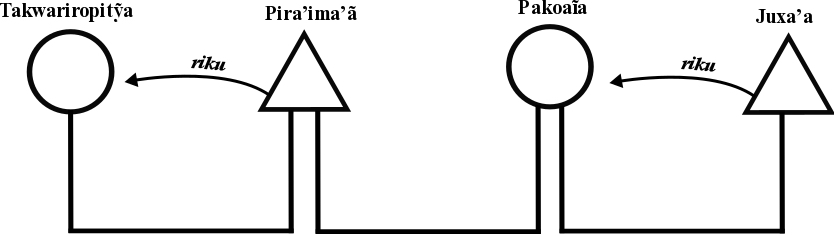
\includegraphics[width=\textwidth]{./imgs/Figura_12}
%\caption{}
\end{figure}

%\includegraphics[width=6.25903in,height=1.77778in]{media/image2.jpeg}

%Figura 12

Enquanto Pira'ima'ã ``pega'' (\emph{pyhy}) e ``cria'' (\emph{riku}) uma nova
esposa, o solteiro Juxa'a, que já havia participado da concepção da
segunda filha de Pira'ima'ã, passa a ser o segundo marido de Pakwa'ĩa;
ao passo que a jovem, e outrora \emph{mihua}, Takwariropitỹa passará a
frequentar a casa de Pira'ima'ã para, a partir de uma boa alimentação,
se transformar em \emph{imirikoa} e consequentemente, \emph{awatea}.
Mesmo esse não sendo um caso de rapto de esposa, nele encontramos algo
semelhante ao fenômeno, a saber, a possibilidade de incorporação por
meio do casamento de uma jovem esposa que ainda não é totalmente humana
(\emph{awatea}), mas, ao contrário, estrangeira (\emph{mihua}). Se o
\emph{riku} é o mais próximo que podemos chamar de conjugalidade, essa
forma é extremamente eficiente para transformar estrangeiras
(\emph{mihua}) em mulheres próximas (\emph{imirikoa}), ao anular as
distâncias por meio do amansamento: rapto, amansamento e casamento podem
aparecer de forma complementar.

Em níveis censitários, os raptos ocorriam com muita frequência antes do
contato, quando os diferentes grupos locais mantinham pouca ou nenhuma
relação entre si. Atualmente, o tema do rapto, \emph{hamirikoa pyhy}
(``apanhar mulher''), está relacionado fundamentalmente aos estrangeiros
\emph{mihua}. E tais mulheres são bastante cobiçadas, como também já
mencionei. Mesmo assim, na vida cotidiana, o verbo \emph{pyhy} (``pegar'')
também pode ser utilizado como sinônimo de ``casar'', no lugar do muito
utilizado \emph{riku}. Diversas foram as vezes em que, ao questionarem
se eu tinha informações sobre os tais \emph{mihua} (os Guajá
``isolados''), os rapazes jovens se gabavam (a mim) de que, caso
encontrassem as jovens desses grupos, as levariam para casa e as
manteriam presas, agarradas ao corpo, dentro de suas redes, mantendo"-as
juntas a si (\emph{pyry}) pelo tempo que fosse necessário. Isso seria
necessário por dois motivos: (1) para que ela não fugisse de volta para
floresta, e (2) para que, bem junta ao homem, se acostumassem um com o
outro. Se uma aproximação dessa qualidade ocorrer (a jovem permanecer
agarrada ao corpo do marido por muitos dias), ela permanecerá esposa
durante muitos anos. Essa é uma ideia muito difundida entre os Guajá,
que estabelecem uma relação direta ao fato de manter"-se junto à alguém
(\emph{pyry})\footnote{O termo \emph{pyry} funciona com uma ``posposição
  adessiva'' (que exprime adjacência), podendo ser traduzido como ``junto
  a'' ou como ``para junto de'', como nos exemplos: \emph{ipyry} -- ``junto
  dele''; \emph{hapyry} -- ``junto a mim'' (Magalhães \emph{op. cit}., p. 56).} como
essencial para que ocorra uma boa relação, seja ela qual for
(paternidade, casamento, e mesmo criação de animais). Vejamos um
exemplo.

Após ser atacada por uma jararaca, a cadela de Ajruhua morreu,
provocando uma grande tristeza em sua dona. Semanas depois, para suprir
a perda da finada cadela caçadora, a mulher conseguiu, por intermédio de
um jovem ribeirinho chamado Chico\footnote{Chico do Cajú, que nasceu às
  margens do rio Caru, é um jovem de 25 anos muito querido pelos Guajá.
  É contratado da \versal{FUNAI} para ajudar em tarefas pesadas do Posto
  Indígena, como a construção de barracões, abertura de roças, limpezas
  de pomar, dentre outras.}, um filhote de vira"-lata como animal de
criação (\emph{nima}) e que, com o tempo, poderia ajudá"-la nas caçadas
de sua família. O pequeno filhote logo já circulava pela aldeia e, como
todo xerimbabo em seus dias iniciais, era a principal distração de todas
as crianças, motivo de orgulho e cuidado dos adultos, principalmente de
sua dona, que ficara muito feliz como seu novo cãozinho. Como eu passava
boa parte dos meus dias de aldeia deitado em qualquer rede que houvesse
disponível na casa de Wirahoa e Ajruhua, inevitavelmente tive aquele
cãozinho comendo as pontas do meu chinelo e lambendo meus dedos sujos de
terra. A todo momento, uma criança colocava o animal no meu colo para
que eu o acariciasse e mesmo brincasse com ele. Devo ressaltar que a
minha convivência com os cães da aldeia Juriti nunca foi das melhores.
Dos vários ataques que sofri --- todos repentinamente ---, uma forte mordida
me deixou sem andar durante pouco mais de uma semana, o que quase me
tirou do campo devido à profundidade da ferida (cuja cicatriz na perna
carregarei durante muitos anos).

É certo que aquele simpático filhote não representava uma grande ameaça,
por isso muitas pessoas puseram"-no em meu colo, a fim de que se
acostumasse comigo, pois quase sempre as crianças se lembravam, em tom
zombeteiro, da mordida que eu havia levado. O jovem Kaawi'ia alertou"-me
para o fato de que, caso o cachorrinho permanecesse um tempo sob os meus
cuidados, se acostumaria com a minha presença e, tão logo crescesse, não
me atacaria, tal como fizera seu predecessor. Devido a meus cuidados, o
animal me tomaria como mais um \emph{jara}, um ``dono''. Argumento não
muito diferente do que \emph{nós} utilizamos para nossos animais
domésticos, focos de cuidado e ``atitudes rituais'', como os gatos e
cachorros (para evocar o célebre artigo de Leach, 1983, p. 174). Por
isso, respondi a Kaawi'ia que minha aproximação com o cachorrinho não
serviria de muita coisa, uma vez que eu não acompanharia seu crescimento
de perto e, inevitavelmente, o animal se esqueceria de mim. Foi nesse
momento que Kaawi'ia me forneceu uma informação relativamente simples,
que até agora parece basilar para entendermos os processos de
transformação de pessoas Guajá. Explico.

Segundo o jovem --- de maneira diferente da relação que os \emph{brancos}
mantêm com seus seres criados, perfilhados e estimados, sejam humanos
(filhos, por exemplo) ou não (animais de estimação, por exemplo) ---,
independentemente do tempo que eu passasse longe do cachorrinho, o fato
de o filhote me cheirar e me reconhecer nesses seus primeiros dias de
infância faria com que ele não se zangasse comigo em sua idade adulta.
Além disso, e segundo essa ideia, os ataques dos cachorros da aldeia a
mim não estavam associados a eu ser um estranho (isso também conta),
mas, principalmente, por eu não ter mantido contato com eles enquanto
filhotes; e agora já era tarde demais. Mesmo que os animais adultos se
acostumassem comigo, nada os impediria de, de uma hora para outra, me
estranharem e atacarem, como fizeram outras vezes. Se o filhote de
cachorro me reconhecesse naqueles seus primeiros meses de infância
enquanto um \emph{jara}, ele não me morderia nem se zangaria comigo na
idade adulta, mesmo eu ficando anos sem voltar para a aldeia. O
importante, ao que parece, seria esse primeiro contato, ainda quando o
ser é um filhote. Kaawi'ia afirmou"-me que não se trata de esquecer ou
lembrar (\emph{imahare} ou \emph{imarakwa}), mas que a convivência é
facilitada a partir desses encontros na fase pré"-matura de cada ser,
seja um animal de criação ou --- como vimos acima --- uma esposa. Certamente
não tenho a intenção de extrair de um registro pequeno princípios
sociológicos amplos, pois não estou seguro de que a explicação seja
essa.

Na mesma direção de ``reconhecer'' e ``lembrar'', eram dirigidos a mim
comentários como: mais cedo ou mais tarde, eu precisaria retornar a
minha casa em São Paulo, pois minha família estaria com saudades; ou que
minha mulher se casaria novamente; e mesmo, que meu sogro se zangaria
comigo\footnote{Comentários semelhantes a tantos outros, que os
  etnógrafos descrevem ao explicar o desconforto moral aludido por seus
  interlocutores por estarem sozinhos no campo.}. Embora nestes
comentários a ideia de esquecimento (\emph{imahare}) nunca estivesse
presente, o problema era sempre a noção de uma dolorida lembrança
(\emph{imarakwa})\footnote{Fato curioso, que ainda estou para entender,
  ocorria toda vez que eu espirrava. Após um espirro, quem estivesse por
  perto comentava comigo, e com todos em volta, em tom de brincadeira,
  que meu espirro era um sintoma de saudades de minha esposa, pois
  quando se pensa muito em alguém sente"-se vontade de espirrar.}, que
poderia me deixar triste e me adoecer. Nesses casos, as ideias de
\emph{pyry} (``junto a''/ ``para junto de'') e \emph{riku} (``estar junto em
movimento'' e/ou ``produzindo uma ação'') parecem centrais ao informarem
tanto o rapto de mulheres quanto a captura de animais.

\emph{Pyry} (``estar junto'' ou ``estar próximo'') é uma categoria que
revela muito da socialidade Guajá, sendo ela mesma a condição do
\emph{riku}. O \emph{pyry} complementa a noção expressa por \emph{riku}:
\emph{riku pyry} ``criar junto a''. O próprio termo de cognação que
exprimiria, em linhas gerais, a ``consanguinidade'', \emph{harapihiara}
``meu consanguíneo''\emph{,} pode ter se originado linguisticamente da
nominalização da posposição \emph{pyry}, traduzido literalmente em sua
origem por ``o que está junto de mim'', pois, como sabemos, para diversos
casos amazônicos a ``consanguinidade'' nada mais é do que uma
ultraproximidade cognática. No entanto, esse termo descritivo, pelo seu
extenso uso como de cognação, teria se lexicalizado e se tornado uma
palavra hoje não segmentável em seus morfemas constitutivos. A
nominalização da posposição \emph{pyry} é realizada atualmente na língua
Guajá por meio da palavra \emph{hapyryhara} (\emph{ha-} + \emph{pyry} +
-\emph{har} + -\emph{a} = ``meu'' + ``junto a'' + sufixo nominalizador
-\emph{har} + sufixo nominal -\emph{a} = ``aquilo/aquele/a que
está junto a mim''). Assim, de acordo com Magalhães (comentário
pessoal), \emph{harapihiara} teria se especializado como termo de
cognação, enquanto \emph{hapyryhara} é o atual termo descritivo para
qualquer objeto que esteja junto a algo ou alguém (uma sacola que esteja
junto a mim, por exemplo).

Desta forma, todas as relações do tipo \emph{riku} são ditas como
aquelas estabelecidas entre seres que se reconhecem como
\emph{harapihiara}. Todo ser dito \emph{nima} é \emph{harapihiara} de
seu \emph{jara}, e vice"-versa. Esse tópico é discutido também por
Cormier ao demonstrar que a relação entre uma mulher e seus animais de
estimação (os macacos, mais especificamente) ocorre entre consanguíneos
(\emph{harypihary}, em sua grafia), pelo fato de os macaquinhos serem os
xerimbabos (\emph{hanima} em sua grafia) das mulheres. Todas as sete
espécies de macacos conhecidos pelos Guajá são tomadas como xerimbabos
(\emph{pets}): macaco"-capelão; macaco"-prego; cairara; sagui
\emph{atamaria}; cuxiu; macaco"-da"-noite e macaco mão"-de"-ouro. Este
último, em pouquíssima incidência na região do rio Caru. Cormier ainda
ressalta que todos os \emph{pets} são chamados \emph{hanima} e que os
macaquinhos são aludidos pelo termo \emph{hamymyra}, ``minha criança'', o
mesmo utilizado pelas mulheres ao se referir a sua prole em geral (\emph{op.
cit.}, p. 115). A autora argumenta que, embora toda ``vida da floresta''
(\emph{forest} \emph{life}) seja considerada um ``parente'' (\emph{kin}),
os macacos de estimação são incorporados mais diretamente ao sistema de
parentesco, sobretudo no nível doméstico. Segundo Cormier,
diferentemente de outros animais, os filhotes de algumas espécies de
primatas podem, após ``incorporados'' a uma família, receber nomes
próprios e apelidos que denotariam parentesco como: ``papai avermelhado'',
para um capelão\footnote{Embora a autora não explique, um apelido como
  esse provavelmente está relacionado à vermelhidão presente nas
  extremidades de seus membros e rabo.}; ``irmã'' ou ``filha'', para um
macaco"-cuxiu (fêmea, imagino); ``cunhadinho'' para um macaco"-da"-noite; e
``marido do sagui'', para o sagui \emph{atamaria} (Cormier, 2003, p. 115).

O próprio morfema -\emph{xa'a}, como vimos no sistema de nomes, também
pode ser estendido aos macacos de estimação. Então, por exemplo, a dona
de um capelão, animais chamados ``\emph{wari}'', poderá chamá"-lo de
``\emph{warixa'a}'', meu ``guaribinha'', ou meu ``capelão parente''. Por
isso, traçar relações de parentesco entre os diversos animais domésticos
é algo que pode acontecer (em tom de brincadeira) nas aldeias, e os
termos \emph{hapihiara} (``irmão''), \emph{imena} (``esposo''),
\emph{hamirikoa} (``esposa''), \emph{imymyra}, \emph{taira} e
\emph{tajyra} (``filhos dele/dela'', a depender do sexo dos pais e do
falante) são acionados a todo tempo, a fim de demarcar relações
específicas entre animais. A forma particular de domesticação desses
macacos encontrada por Cormier, cuja relação de parentesco é tida como
central ao seu trabalho, denota menos uma ``proximidade de natureza entre
humanos e animais'' (como defende a autora), mas sim, outra forma de
relação que postula certas homologias relacionais. Se pensarmos junto
com a ideia de \emph{riku}, a citada nominação dos macacos fará parte de
um sistema de classificação que recusaria o par natureza e sociedade,
uma vez que ``a natureza e a sociedade não são neste caso separadas por
fronteiras ontológicas'' (Descola, 1992, p. 116).

Como exemplo, o sagui (\emph{atamaria}) de Panyxĩa era mantido preso
pelo pescoço, amarrado a uma viga de sua casa. Sua dona o mantinha assim
por o animal ser \emph{imahy} (nervoso/raivoso/``brabo'') e fugir
constantemente para encontrar o sagui de sua avó, Amỹ Piirawãja. Ambos
eram machos e quando se encontravam gritavam muito e reviravam os
objetos. Segundo Panaxĩa, o sagui de Amỹ Piirawãja e o seu eram
\emph{harapihiara} entre si, por isso permaneciam juntos para
\emph{wata} (caminhar/caçar/coletar); \emph{wata} \emph{pyry} (``andar
junto''), para ser mais preciso. Quando lhe perguntei se quando sem sua
coleira o sagui não fugiria para a floresta para encontrar outros
cognatos (\emph{harapihiara}), disse"-me que os saguis da floresta eram
\emph{mihua} (selvagens) para seu sagui, portanto, só seriam
\emph{harapihiara} os saguis que viviam naquela aldeia. Isto sugere que,
tal como as relações de parentesco, a relação entre dois animais só pode
ser traçada a partir da que cada um estabelece em seu mundo. Mesmo os
termos de parentesco ``transpostos'' para as relações animais, tal como
vimos no exemplo de Cormier linhas acima, são dirigidos de acordo com o
caso, e não há uma regra absoluta que prescreva substância e forma. Em
outras palavras, cada xerimbabo será parente de outro de acordo com a
espécie, a história, a forma de domesticação, o humor de sua dona, e
outros detalhes.

Ainda no caso dos animais de criação, como em outros povos da América do
Sul (Vander Velden, 2012, pp. 112--117), ao chegar nas aldeias os animais
quase sempre são modificados. Aves têm parte de suas penas retiradas ou
aparadas para que não consigam fugir, bem como as pontas seus bicos são
cortados com tesouras para que, ao bicarem, não machuquem sobretudo as
crianças. As afiadas garras de quatis são retiradas ou lixadas com lima.
Paquinhas e filhotes de cotias têm seus dentes serrados (também com
lima) para que as pontas cortantes não firam ninguém. Queixadas e
caititus devem ficar bem amarrados ou presos em currais, para que o
corre"-corre dos bichos não transforme a aldeia em uma grande bagunça e
gritaria; esses animais comem tudo o que encontram pela frente, de lixo
a pintinhos. Apenas os macacos parecem não sofrer tantas intervenções,
como cortes e outras injúrias. Com os macacos nada se faz. Quando muito,
são presos com cordinhas por algum tempo, até ficarem mansos. Os que
nunca se acalmam permanecerão amarrados até um dia em que serão soltos.
Não basta, portanto, ``estar junto'', é preciso que essa proximidade não
cause danos.

%\textbf{Foto do quati sendo mexido}
\begin{figure}[!ht]
\centering
  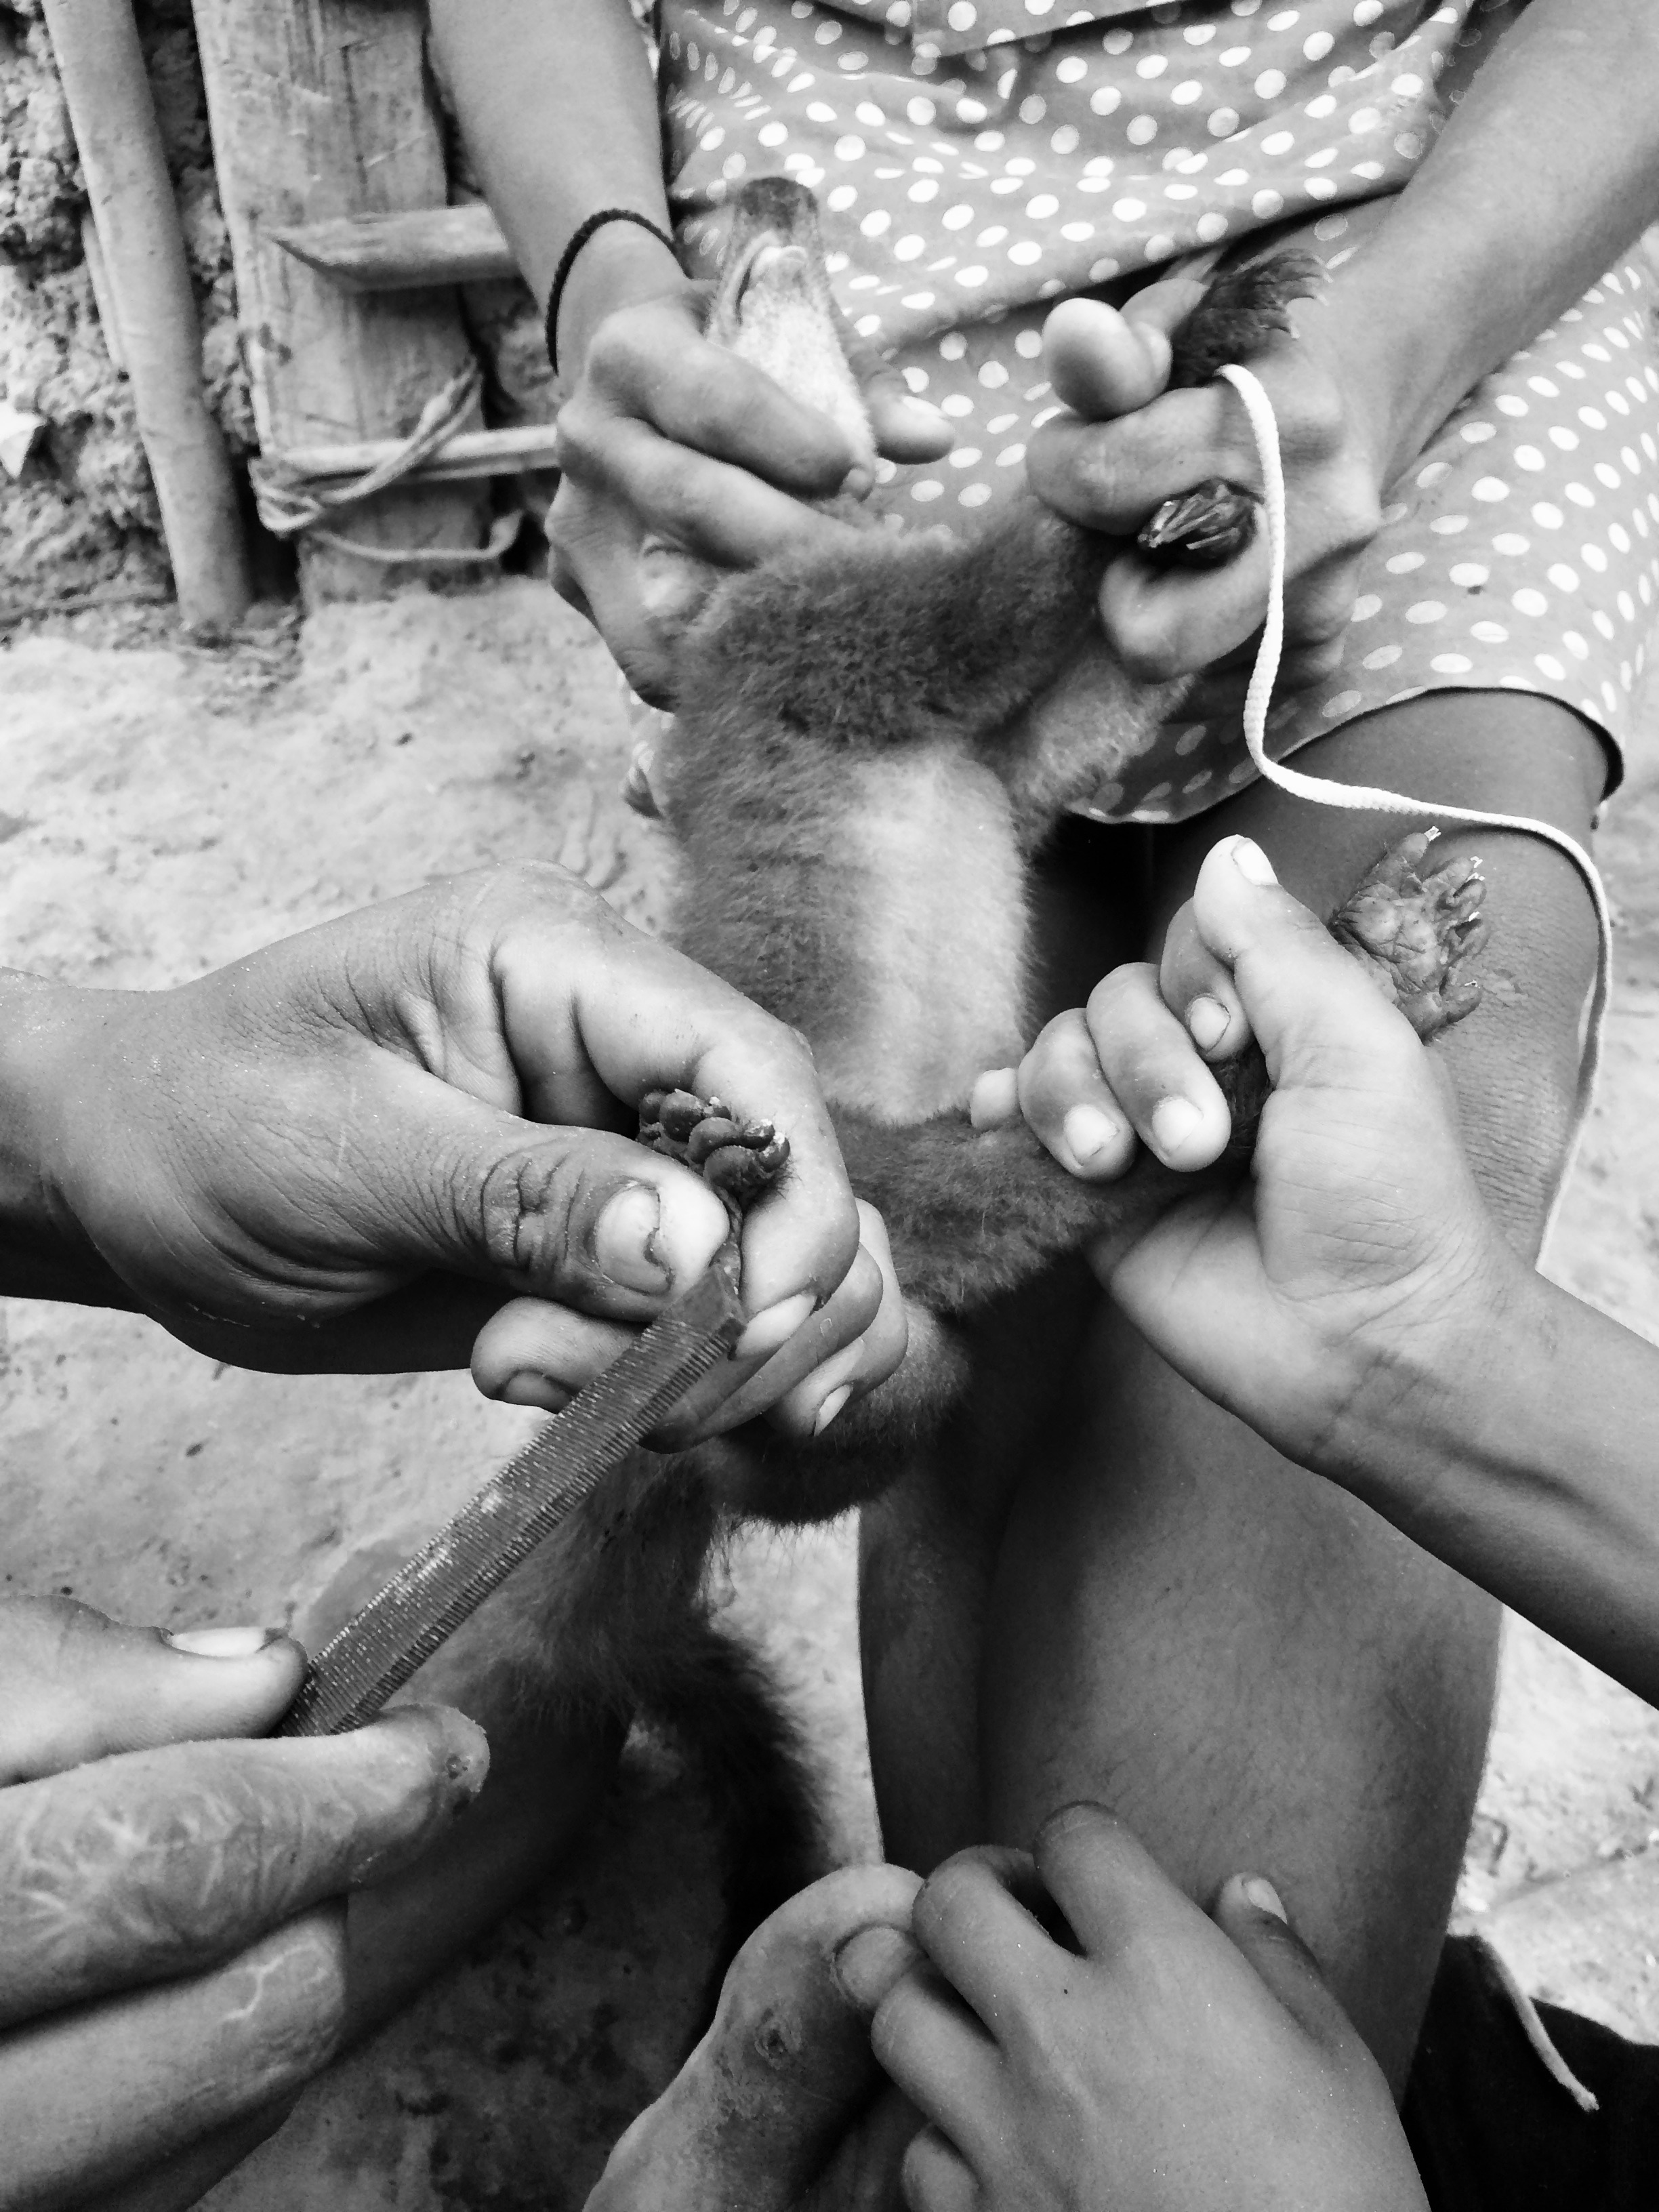
\includegraphics[width=\textwidth]{./imgs/IMG_0343}
\caption{As unhas afiadas do quati de Xikapiõ precisam ser limadas para não ferir a
sua dona (aldeia Juriti, 2016).}
\end{figure}

A vida desses animais na aldeia depende de --- digamos assim --- acordos
interespecíficos entre seus donos humanos e essas criaturas. De maneira
geral, a primeira reação dos animais é resistir à criação, e muitos
conseguem fazê"-lo --- escapando ou morrendo --- causando frustração naquelas
que desejavam ser donas (\emph{jara}), criadoras. Os animais têm medo
quando chegam à aldeia e muitos simplesmente não querem comer, morrendo
também de fome. Animais como o jacaré, por exemplo, são difíceis de
domesticar sobretudo diante de sua dieta exclusivamente carnívora, às
vezes complicada para ser administrada pelos humanos. O último jacaré
capturado que vi em uma aldeia recusou as carnes (de caititu e cotia)
que lhe eram oferecidas e morreu por inanição\footnote{A outra opção
  seria deixá"-lo se alimentar à noite, com sapos e outros animais que
  lhe apetecem, mas isso estava fora de questão por motivos
  autoevidentes. Ninguém deixaria um jacaré solto na aldeia à noite.}.
Não apenas o jacaré em questão, mas diversos macacos, aves como
periquitos, araras, inhambus, e mamíferos como pacas e cotias, durante
os primeiros dias da nova vida se opõem à mudança na dieta. Notem que
para cada animal, ou conjunto de animais, algumas regras são obedecidas.
Algumas espécies comem farinha, outras não. Mingaus, carnes, frutos, e
até refeições como as humanas, cada um dos alimentos vai variar de
acordo com os hábitos da espécie. Para alguns a comida de gente
(\emph{awa nimi'ua}) bastará, para outros a alimentação será mais
seletiva e específica.

Os animais da aldeia precisam aprender a ser animais de aldeia, e nem
todos estão dispostos a isso. Existem diversas maneiras dos bichos
resistirem, fugirem ou sabotarem a nova vida de cativos. Os filhotes de
cotias podem roer as cordas que lhe prendem e fogem de volta para a
floresta. Os quatis são muito bravos e podem ser violentos com as
crianças. Além disso, comem os pintinhos que vivem soltos na aldeia, e
podem roubar ovos de galinhas e de outras aves como o jacu. Esses quatis
de criação também são um problema dentro de casa pois mexem em toda a
comida, furam os sacos e espalham farinha por todos os lados. Assim como
os quatis, os filhotes de porcos também querem comer pintinhos da aldeia
e, por serem fortes, quase incontroláveis em sua corrida, precisam viver
em currais (\emph{hakãnã'ã}). ``Os porcos até parecem gaviões'', me
disse um amigo certa vez, dada a avidez dos queixadas por pintinhos. Os
macacos"-prego são muito bravos, ao mesmo tempo que habilidosos, uma
combinação que não tem como dar certo. Mexem em machados, facas, cordas
e até moto"-serras. São eles os mais ciumentos e atacam os filhos de suas
donas. Os macacos"-cairara, por sua vez, adoram ficar brincando e são
sempre comparados às crianças. Os macacos cuxiú"-preto são grandes
companheiros de caminhada, calmos, são capazes de manter uma grande
conexão com suas donas nas caminhadas. Os Guajá sempre lembram como os
cuxiú são bons companheiros de caçada. Um dos animais mais exigentes é o
capelão. Sua domesticação sempre será difícil pois se negam a comer
qualquer alimento relacionado à dieta humana, além de serem ``chorões''
(\emph{já'ohara} ``chorador'') e terem muita ``saudade''
(\emph{imarakwa}, ``pensar'') da vida na mata. Os capelães morrem muito
facilmente na aldeia. É uma tarefa difícil criá"-los. Não comem farinha,
milho ou arroz, e nem mesmo as frutas dos novos pomares (plantados com a
ajuda de não indígenas) como manga e jaca. Os capelães só gostam da
comida do mato.

\section{Familiarização, Criação}

Um modelo elaborado para a Amazônia a respeito das relações entre
``donos'' (ou ``senhores'') e ``criaturas'' (ou ``xerimbabos'') foi o que Fausto
denominou ``Predação Familiarizante''. A partir da relação entre os
humanos e seus xerimbabos oníricos, que auxiliam os primeiros em suas
curas, Fausto observa um aspecto fundamental da socialidade ameríndia, a
saber, as ``relações assimétricas de controle, real ou simbólico,
conceitualizadas como'' formas de adoção e pertinentes a quatro domínios:
caça, xamanismo, ritual e guerra (Fausto, 2001, p. 413). Não vou
discutir em detalhes o modelo do autor, uma vez que, além de ser de uma
ambição generalista, foi retomado de forma comparativa em um importante
artigo (Fausto, 2008)\footnote{O modelo de Fausto dialoga diretamente
  com a ideia de ``economia simbólica da predação'', tal como desenvolvido
  por Viveiros de Castro. Assim formula o autor: ``Em resumo, se de fato
      é possível falar em uma economia simbólica da predação (Viveiros de
      Castro, 1993), é preciso desenvolver seu complemento --- que não é uma
      teoria da reciprocidade equilibrada, mas sim das relações assimétricas
      do tipo pai"-filho ou sogro"-genro, constituídas por meio do homicídio e
      do sonho"-transe. A predação é um momento do processo de produção de
      pessoas do qual a familiarização é outro. Não se compreenderá o
      sentido da guerra ameríndia por sua redução às relações simétricas de
      troca, mas sim, pela construção de um \emph{modelo das relações
      assimétricas de controle simbólico}'' (Fausto, 2001, p. 418, grifos do
  autor).}. Ao apresentar ``a operação de aquisição do poder xamânico
    como um processo de familiarização de entes extra"-humanos, com
    frequência associados à predação e ao canibalismo'', o autor nota que ``a
        relação familiar é modelada por duas relações assimétricas que envolvem
        controle e proteção: aquela entre pai e filho e/ou aquela entre dono e
        bicho de estimação'' (Fausto, 2001, pp. 415--416). Das formas que preveem o
esquema da familiarização além dessas duas restariam: o controle
simbólico sobre objetos rituais e ornamentos corporais (Ikpeng, Tukano);
a dessubstanciação de animais caçados a fim de lhes retirar as armas
(Makuna); os cativos de guerra (Tupinambá) e crianças raptadas (Ikpeng,
Curripaco), tratados como xerimbabos; e, por fim, o processo de
apropriação/domesticação do espírito de uma vítima/presa humana pelo seu
carrasco, como ocorre em diversos povos (como os Araweté, Nivacle, Wari)
(\emph{idem}, p. 417). A doutrina dos cantos de cura \emph{karahiwa}, dados
pelos \emph{akwawá} (inimigos oníricos que auxiliam o xamã), entre os
Parakanã, ``ou a ideia de alteração (devir"-outro) do matador araweté''
prescrevem um ordenamento semelhante entre as operações de domesticação
no xamanismo e na guerra; e ``ambas são parte de uma economia
generalizada de produção de pessoas'' (Fausto, \emph{op. cit}., pp. 417--418). Tal
como no \emph{riku} Guajá:

\begin{quote}
\emph{os temas principais são ontológicos: aquisição de alma e virtualidades
de pessoas, nominação e existência, desenvolvimento das capacidades
plenas da pessoa e maturação, controle sobre os processos mórbidos e
longevidade, conquista sobre a morte e imortalidade (\emph{idem})}.
\end{quote}

Fausto utiliza o modelo da relação entre senhores e xerimbabos, que
prescreve um vínculo de proteção e adoção, como constituinte de um tipo
de socialidade particular encontrada em diversos grupos amazônicos, mais
especificamente, no xamanismo Parakanã. Tal modelo, denominado
``predação familiarizante'', atesta de forma bem sucedida que as
diversas relações, sejam entre matador e vítima pós"-homicídio ou entre
xamãs e espíritos auxiliares (dentre outras), são pensadas como uma
forma de ``filiação adotiva'':

\begin{quote}
\emph{A relação prototípica de controle nas sociedades ameríndias não é,
porém, a do mestre e do escravo, mas a do senhor e do xerimbabo, que é
exercida praticamente na familiarização de animais e no rapto de
crianças estrangeiras. Estes, porém, não são senão casos particulares de
uma estrutura relacional mais ampla, que envolve a familiarização do
princípio vital da vítima na guerra e de espíritos de animais no
xamanismo (Fausto, 2001, p. 539)}.
\end{quote}

O autor não menciona a relação marido"-esposa em seu primeiro esquema
(2001) relacional, diferentemente do que encontrei entre os Guajá
(embora, talvez não seja por acaso o modelo da predação familiarizante
surgir a partir de uma sociedade que prescreve justamente o casamento
com \versal{ZD}). No entanto, em uma análise mais recente Fausto insere a
``maternidade'' e a ``matrimonialidade'' no artigo em que retomou as ideias
de ``maestria'' e ``domínio'' como fundamentais à compreensão das
socialidades amazônicas (Fausto, 2008). Para o autor, a ``maternidade'' é
tratada como um caso particular das relações de maestria e ``se expressa
nas figuras da mãe da caça (ou de alguma espécie em particular) ou da
mãe de plantas (em especial, as alucinógenas). Contudo, o uso da
categoria `mãe' para designar entidades similares aos donos é restrita
etnograficamente, além de não se aplicar ao espectro mais geral de
relações de domínio que caracterizam a noção de dono"-mestre'' (Fausto,
2008, p. 350).

O caso Guajá questiona o ``absolutismo'' das formas \emph{dono"-mestre} ---
sugerindo uma multiplicidade de formas que não se sobrepõem --- e concebe
a maternidade (fisiológica) a partir de um modelo onde o que prevalece é
a relação \emph{riku}, que nem sempre será uma relação assimétrica de
``controle simbólico'' (Fausto, 2001, p. 418). Em outra palavras, toda
relação \emph{riku} estabelecida entre um \emph{jara} e um \emph{nima}
é, sim, assimétrica, da mesma forma que Fausto pensa as relações de
maestria; porém nem sempre o que estará em jogo será domínio e controle.
Por exemplo, a relação entre um \emph{karawara} dito ser, no céu,
\emph{jara} de determinado animal terreno, como o \emph{Makaro}
\emph{Jara} (gente"-pomba"-galega) e seu correlato terreno, não é uma
relação de controle. As qualidades desse \emph{karawara} estão
relacionadas ao fato de ele ser um exímio caçador de porcos (como
veremos no último capítulo) e não por controlar as pombas"-galegas
(\emph{Patagioenas cayennensis}) terrenas. Dessas últimas, o
\emph{Makaro Jara} é apenas uma ``versão celeste'' ou ``duplo'', como venho
chamando aqui. Ainda assim, as pombas"-galegas (\emph{makaro}) terrenas
são ditas \emph{nima} de \emph{Makaro Jara}, mesmo não sendo controladas
por esse. Isso sugere que o \emph{riku} relaciona seres sem
necessariamente produzir uma relação de poder, domínio ou controle, mas
sim, de assimetria, tendo"-se em vista que o \emph{Makaro Jara} é humano,
e o \emph{makaro} terreno não. E as versões humanas, ou que pelo menos
se consideram como tal, são as que se veem como \emph{jara}.

Fausto observa que o conceito de \emph{maestria} ``é tão central à
compreensão das sociocosmologias indígenas quanto a afinidade'' (Fausto,
2008, p. 330). No caso Guajá, parece"-me que ``maestria'' e ``afinidade''
(no sentido de ideias que determinam o casamento, em uma teoria da
relacionalidade generalizada, nas palavras de Viveiros de Castro, 2002)
não podem ser pensadas isoladamente. E quanto à aliança especificamente,
ela é para os Guajá uma forma de ``maestria'' (\emph{riku}). Ao apontarem
que casar é \emph{riku} (ação que está em vários lugares, produzindo
afecções entre seres de diferentes ordens, inclusive entre um homem e a
filha de sua irmã, \versal{ZD}), os Guajá asseveram que a aliança é um caso
particular da maestria. Se a intenção é justamente ``fazer parentesco
querer dizer outra coisa'', as ideias Guajá para o casamento ``não só
determinam outros referentes que os nossos, como envolvem outros
componentes'' (Viveiros de Castro, 2002, p. 407).

Quanto à ``matrimonialidade'' (nas palavras de Fausto), o autor a sugere a
partir da perspectiva do xamanismo, ``pois o xamã constitui verdadeiras
famílias espirituais: tem uma esposa, afins e gera filhos"-espíritos''
(Fausto, 2008, p. 351). E, a partir do exemplo Nambikwara"-Mamaindê, traça
uma relação entre ``matrimonialidade'' e ``familiarização'':

\begin{quote}
\emph{Os Nambikwara"-Mamaindê nos fornecem o exemplo mais sugestivo dessa
assimilação entre casamento e familiarização (Fausto, 2001b). A
esposa"-espírito, que é um jaguar, é denominada da \emph{mãindu} (``minha
criação'' ou ``meu xerimbabo'') pelo marido"-xamã. Como era de se
esperar, observa"-se também aqui a instabilidade posicional que marca, em
geral, as relações de mútua constituição entre xamãs e auxiliares: ``não
se sabe ao certo quem está `criando' quem. Embora o xamã chame a
mulher"-espírito de `minha criação'; ao partilhar comida e enfeites
corporais com ela, o xamã indica que é ele quem está sendo `criado' por
ela'' (Miller, 2007, p. 199) (Fausto, 2008)}.
\end{quote}

De fato, o exemplo acima é rico ao apontar um mecanismo que, se
cosmopolítico para os Nambikwara"-Mamaindê, para os Guajá está no plano
da sociologia (embora, como ainda veremos, casamentos com mulheres
celestes também podem ocorrer), em que as esposas são tidas literalmente
como ``minha criação'' ou, em uma tradução literal, ``objetos do meu criar''
(\emph{imirikoa}). E se a cosmologia Mamaindê propõe uma recíproca na
relação de ``criação'' entre maridos"-xamãs e esposas"-espíritos, a
sociologia Guajá --- bem como a Tupinambá, como vimos acima --- também
defende que maridos ``criam'' esposas, esposas ``criam'' maridos.

Uma mulher mais velha (muitas vezes, viúva) pode propor casamento a um
jovem promissor da mesma forma que os homens fazem com as mulheres:
\emph{jaha ariku ta ni pyry} (eu quero ficar com você/ te criar). Foi
assim, inclusive, que Ajruhua e Wirahoa se casaram, ela com 24 e ele com
16 anos. Um casamento recorrente nos padrões Guajá, em que mulheres
adultas com 25, 30 desposam rapazes jovens de 14, 15 anos. Por um lado,
esse e outros arranjos são concomitantes ao contato, momento em que
historicamente os Guajá foram dizimados e sofreram uma drástica
depopulação, o que inflete diretamente nos arranjos matrimoniais
(incesto, mudanças no padrão residencial, poligamia onde não havia,
etc.). A literatura etnológica está repleta de exemplos como esse (para
dois casos Tupi"-Guarani, ver Müller, 1993; e Wagley, 1988). Mas recorrer
ao argumento da crise do contato esconde as próprias preferências das
pessoas. Diz"-se das mulheres ``criarem'' seus maridos, porém o argumento
não me foi fornecido com todos os detalhes que adquiri do casamento a
partir do ponto de vista masculino. O fato de eu ser homem não deixou
que eu apreendesse com apuro o \emph{riku} (casamento), tal como as
mulheres o mantêm com seus homens. Por outro lado, os efeitos dessas
criações (de mulheres sobre homens), se tornam aparente todo o tempo, e
novas uniões inter"-geracionais são desfeitas muitas vezes antes de
começar. Não apenas os efeitos, mas novas linhas de fuga são traçadas a
cada novo arranjo. Podemos ver isso no caso de Jawa'nĩa, um jovem que
com apenas 15 anos saiu de sua aldeia de origem para ser criado pela
mulher Ximirapi na aldeia Tiracambu. Ela tinha cerca de 35 anos na
época. Uma vez na aldeia, vivendo, sendo criado por Ximirapi, o rapaz se
``acostumou'' com uma outra jovem, mais nova até do que ele, com quem
decidiu se casar, largando para trás a ``mulher velha'', voltando à sua
aldeia de origem com a jovem mulher\footnote{Hoje em dia (2017), alguns
  anos depois, ele voltou à viver na aldeia de sua esposa.}.

Podemos dizer que há uma assimetria nesta relação marido e esposa que
escapa à pura dominação masculino"-feminino e instaura um tipo de
socialidade intersexual, que no plano terminológico prescreve a esposa
(\emph{imirikoa} ``aquela que eu crio'') como alguém que é resultado da
ação \emph{riku}; porém no plano da ação, apesar de não aparecer na
terminologia, homens indubitavelmente também são ``pegos'' para
``criar''. Encontramos nos Guajá, tanto homens criando mulheres quanto
vice"-versa. Por isso a mulher enquanto puro ser criável (e não que cria)
parece estar fundamentalmente no plano da língua, enquanto a etnografia
prefere mostrar outra coisa.

\section{A ficção do dono}

Para finalizar o capítulo, problematizo etnograficamente a discussão
sobre os ``donos'' na Amazônia; mas antes, para auxiliar na análise,
discuto alguns casos correlatos ao \emph{riku} Guajá encontrados em
povos falantes do Tupi"-Guarani, particularmente. Não compete a este
trabalho avaliar os problemas e as soluções impostos a outras
etnografias; e os questionamentos e soluções que venho encontrando para
o caso Guajá não precisam ser completamente replicáveis a outros
contextos etnográficos, correlatos ou não. Porém, algumas conexões ---
ainda que parciais --- podem ser traçadas entre o caso Guajá e outros
Tupi"-Guarani, uma vez que, apesar das claras diferenças entre esses
coletivos (como todos sabemos), encontramos de maneiras transversas
aspectos que dialogam.

Linguisticamente, o \emph{riku}, como um termo que exprime relações
particulares, está presente em algumas outras línguas da família
Tupi"-Guarani, como o -\emph{reko} do Guarani Mbya como vimos acima, ou
na formação de palavras associadas ao termo como o termo para esposa,
\emph{he"-remirikó}, na língua Tenetehara (Wagley e Galvão, \emph{op. cit}.).
Tal ideia experimentou diferentes traduções, exprimindo subjetividades
diversas, e, como observamos, as traduções linguísticas do tipo ``estar
junto a'', ``estar com'' (ou qualquer outra semelhante), no caso Guajá, não
seriam suficientes para a compreensão da relação como um todo. Meu
trabalho não é o primeiro a abordar o interesse de um povo para com essa
concepção de relação encarnada na forma \emph{riku}. O exemplo mais
relevante para o caso é a ideia de \emph{werekio}, encontrada entre os
Zo'e, um povo linguisticamente próximo aos Guajá\footnote{Segundo
  Rodrigues, ao lado de outras línguas, tanto o Guajá quanto o Zo'e
  pertencem ao subgrupo \versal{VIII} (oito) da família Tupi"-Guarani, o que os
  fazem menos distantes no plano intrafamiliar.}. Havt traduz o termo
\emph{werekio} como ``estar com'' e ainda ``tomar como esposa'', e lembra
que, tal como entre os Guajá, é um termo que aparece ``com frequência em
outros contextos (\ldots{}), não necessariamente envolvendo um matrimônio''
(Havt, 2001, p. 48). Para a autora, ``quando um Zo'e fala em
\emph{werekio} ele está se referindo a uma adoção, no sentido de uma
incorporação daquele elemento a seu viver. Mais adiante, esse termo vai
ser encontrado referindo"-se a um cônjuge, ao porte de algum utensílio,
ao uso de uma técnica de apropriação e/ou uso do ambiente, aos cultivos
das roças, enfim, a qualquer aspecto que possa ser definido como parte
(ou que possa fazer parte) da vida, de um jeito de ser'' (\emph{idem}, grifos
meus). Tal como encontramos entre os Guajá, os Zo'e se referem a
diferentes atividades mediante um mesmo termo capaz de expressar ideias
próximas, embora diversas. Termo pelo qual são tratadas várias ações,
não por uma escassez de outros específicos a elas, mas por ser o índice
de outra propriedade relacional, isto é, sugerindo uma homologia nas
práticas. Porém, a despeito da precisão etnográfica da autora, cujo
cognato \emph{werekio} se relaciona ao cultivo das roças, à
conjugalidade, à posse de objetos, dentre outras possibilidades, Havt
prefere precisá"-lo por meio de ideias pré"-existentes, como ``jeito de
ser'', ou mesmo ``costume'' (Havt, \emph{op. cit}., pp. 48--50, nota 36). Esses
termos, para o caso Guajá, soariam um pouco vagos, uma vez que se trata
muito mais de um sistema de ação, que relaciona e interfere na vida das
pessoas, do que um ``estado'' de vida ou um ``costume''. Segundo Havt, o
\emph{processo de amansamento}, como a incorporação de um xerimbabo, os
cultivos das roças, até a incorporação dos afins, corresidentes e os
\emph{kirahi} (os não indígenas) a um grupo local, ``guarda estreita
relação com a noção de (\emph{were})-\emph{kio}'' que também faz
``referência ao tomar alguém como cônjuge'' (\emph{idem}, p. 65). Para Havt, o
\emph{werekio} faz:

\begin{quote}
\emph{(\ldots{}) referência a algo que é incorporado como se fosse um hábito,
um costume. Por exemplo: faz parte do \emph{jeito de ser dos Zo'e}
portar o adorno tembetá (\emph{embepot}), feito de madeira poturu, na
região pré"-labial inferior; fazer de alguém seu cônjuge efetivo é
expresso como \emph{werekio}; os cultivos atuais --- relacionados em
diversas narrativas ao contato com os vizinhos \emph{Tapãaj} que se
tornaram inimigos --- são considerados como adoções, da mesma maneira que
as flechas atuais; a adoção, possibilitada pelo contato pelos
\emph{Kirahi}, de machados com lâmina de metal também é tratada em
termos da incorporação desse utensílio ao jeito de ser zo'e (\emph{idem}, p. 66, grifos meus)}.
\end{quote}

Novamente, ideias como ``jeito de ser'', ``hábito'' e ``costume'' são
utilizadas para explicar esse conjunto de ações. Tudo se passa como se o
\emph{werekio} zo'e fosse algo dissociado das próprias ações de adotar,
plantar, portar, casar e incorporar. Como exemplo, a incorporação de
utensílios vindo do mundo dos não"-índios ``é tratada em termos da
incorporação desse utensílio ao jeito de ser zo'e''. No final de sua
análise, a autora sintetiza o \emph{werekio zo'e} como a ``incorporação
de algum aspecto como hábito'' (\emph{idem}, p. 66). De forma diversa, o que
proponho para o caso Guajá é que não há ``jeitos de ser'', mas
\emph{formas de agir} (e outras formas de ação): incorporação, adoção,
relação de casamento, dentre outras que elenquei nos parágrafos
anteriores.

Para os grupos Guarani, os termos \emph{teko} e -\emph{reko} também
foram traduzidos, em diferentes autores, a partir de ideias como ``modo
de ser'' e ``jeito de ser'' e se vinculam a ``uma outra (noção) que assume,
em grande parte das análises, uma conotação espacial forte, a de
\emph{tekoa}'', o local de exercício do \emph{teko} (Pissolato, \emph{op. cit}.,
pp. 105--106):

\begin{quote}
\emph{Para o termo \emph{teko}, Montoya apresenta os seguintes significados:
``ser, estado de vida, condição, estar, costume, lei, hábito'' (Montoya,
1991, p. 13), que Melià recupera para afirmar esta noção como expressão
mais acabada de uma ``identidade guarani'' singular (Melia, 1991, p. 13)
(extraído de Pissolato, 2007, p. 108)}.
\end{quote}

De acordo com Pissolato, o que parecem informar muitos desses autores ``é
a noção de que há um `sistema' (uma outra tradução possível para
\emph{teko}) englobando uma ética religiosa, uma forma econômica, um
código de solidariedade, enfim uma orientação para o estar"-no"-mundo
deixada pelos antepassados'' (\emph{idem}). O \emph{teko} nesses casos se
comporta ora como a própria vida (ser, estar, estado de vida, condição),
ora como um dado da cultura (costume, lei, hábito), tal como aparece em
Havt a respeito do \emph{werekio} dos Zo'e (``costume'' ou ``hábito''). O
``nosso modo de ser/viver'', \emph{nhandereko}, ou o ``meu ser/minha vida'',
\emph{xereko}, são as formas pelas quais as ideias particulares sobre a
vida/costume das pessoas, uma vez que de acordo com os \emph{Mbya}, são
que cada pessoa tem seu \emph{jeito}, seu \emph{costume} (\emph{idem}, grifo da
autora)\footnote{Em sua forma contemporânea, o \emph{nandereko} (``nosso
  modo de viver''), é traduzido pelos próprios Guarani como ``Cultura'', e
  se filia a um conjunto de reivindicações desses coletivos, articulando
  políticas públicas, projetos de meio ambiente e atividades culturais
  (como a gravação de \versal{CD}s e apresentações públicas (sobre estes pontos,
  ver o interessante trabalho de Macedo, 2010).}.

Para os Guajá, diversamente dos exemplos Guarani e Zo'e, o \emph{riku} é
um sistema de ação --- por exemplo, na adoção e no casamento ---, e não um
mecanismo que possibilite uma vida a partir de um conjunto de costumes
ou hábitos; ele é um método de produção da vida coletiva (Lima, 2005,
p. 96), e não um ``jeito de ser'' (até porque não existem correspondentes
do verbo ``ser'' nas línguas Tupi"-Guarani). Com isso, sugiro que o
\emph{riku} deva ser pensado a partir de teia virtual de relações que
compõem a socialidade amazônica\footnote{Recusando o par ``Indivíduo'' e
  ``Sociedade'', tomo de empréstimo a ideia de ``socialidade'' tal como
  formula Marilyn Strathern (2006, pp. 40--41), pensando os ``indivíduos''
  não enquanto sociais, mas como pessoas conceitualmente ligadas às
  relações que as unem, pois elas ``são integradas por relações''
  (Viveiros de Castro, 2007, p. 107); subprodutos e produtores de suas
  interações que, no caso Guajá, são estabelecidas com (e entre) seres
  de diferentes ordens, escapando à ideias de coesão social ou mesmo
  sociedade.} em geral, e Guajá, de forma específica (animais, humanos,
deuses; e também, fenômenos como o vento, alimentos como o mel, dentre
tantos outros, como já apresentados aqui). O \emph{riku}, parafraseando
Lima, é uma realidade concreta da vida humana. É menos uma ideia
abstrata do que --- se for razoável destacar --- um princípio sociológico
não menos real do que tantos outros de nossa disciplina, como
``linhagens, classes, tabus, bruxos e o casamento preferencial dos primos
cruzados'' (Seeger, \emph{apud} Lima, 2005, p. 94).

Uma característica do \emph{riku} Guajá, em comparação a outras relações
que ocorrem na Amazônia, é o fato de tal ideia se associar tanto a uma
teoria da relacionalidade generalizada --- a saber, as formas de aliança e
parentesco, alternativas a um modelo genealogista"-terminológico, tal
como antevisto nos trabalhos de Viveiros de Castro e consagrados em sua
teoria da afinidade (Viveiros de Castro, 2002, p. 422) --- quanto ser
parte constitutiva de uma ontologia da familiarização, que prescreve o
mundo permeado por relações entre ``donos'' e ``criaturas'', tal como
aparece nos trabalhos de Descola (2006), Fausto (2001) e Gallois (1988).
Fausto recorda que as relações do tipo ``maestria"-domínio'' foram
``relegadas às notas de rodapé das etnografias ou reduzidas a uma simples
categoria ontológica, a dos donos ou mestres da natureza'', e seu artigo
``visa a mostrar, ao contrário, que a relação de maestria é tão central à
compreensão das sociocosmologias indígenas quanto a de afinidade''
(Fausto, 2008, pp. 329--330). Porém, para o caso Guajá, se pensarmos a
afinidade como regida pelas categorias do próximo e distante; aliados e
inimigos; cognatos e não"-cognatos, dentre outros termos diferenciantes,
o \emph{riku} seria, antes de tudo, uma forma que permite a
transformação desses ``distantes'' (\emph{hapihianã}) em ``próximos''
(\emph{hapihiara}). O \emph{riku}, ao menos para os humanos, também ``é a
desconstrução da afinidade potencial'' (Viveiros de Castro, 2002, p.
447), uma busca infinita pela proximidade cognática, em que, do ponto de
vista de ego masculino, estranhas devem ser transformadas em
irmãs/sogras (\emph{xikari}) e sobrinhas, em esposas (\emph{imirikoa});
ou do ponto de vista da aldeia, animais devem ser transformados em
``parentes'' (\emph{nima}, \emph{hapihiara}). E o \emph{riku} ainda
ajudaria a refletir por que animais (\emph{nima}) são deuses
(\emph{karawara}); ou humanos (\emph{jara}) possuem duplos celestes
(\emph{nima}), informando a própria zoologia ao considerar que algumas
espécies (\emph{jara}) são mais próximas de outras (\emph{nima}). E todo
ser, a partir desse mecanismo replicante e de infinita reprodução, tende
e a se aproximar de outro ser. No plano local, o \emph{riku}, essa
``afinidade intensiva'' (Viveiros de Castro, 2007) atua nas relações
humanas; e o sistema de aliança Guajá só poderá ser compreendido se
entendermos esse verbo que, como vem mostrando esta etnografia, ordena
tanto o parentesco quanto outras relações.

Devo salientar que iniciei minha pesquisa de doutorado interessado no
sistema de parentesco (categorias, regras e práticas) Guajá, porém, uma
vez entre eles e ao segui"-los, deparei"-me com tais noções, o que colocou
a discussão sobre parentesco como ``ponto de partida''. Ou, sendo mais
direto, dificilmente entenderemos o que é --- por exemplo --- o
``casamento'' aqui sem antes entendermos como as pessoas (\emph{awatea})
concebem e constroem suas relações. E quando as penso aqui, passando de
uma a outra, tenho a intenção de destacar o caráter multinatural e
perspectivo presente nestas relações que, como já salientado por outros
autores (ver Viveiros de Castro, 1996, Lima, 1996), é fundamental para o
entendimento de uma sociocosmologia como esta que estamos observando. O
parentesco Guajá seria uma dessas ``teorias não"-biológicas sobre a
vida'', como escreveu Viveiros de Castro em um artigo recente (2009).
Isto significa que para apreendê"-lo se faz necessário incorporar não só
o ``método genealógico'', mas também o conjunto de ideias que
caracterizam os Guajá como um grupo diferente de --- por exemplo --- nós
mesmos.

A ideia de um mundo repleto de entidades distintas entre si,
relacionadas como \emph{jara} e \emph{nima} (cria), relações que
circunscrevem a humanidade e nas quais a tradução de \emph{jara} nem
sempre será ``dono'', mas sim ``criador'', ``quem anda junto'', ``duplos'',
``cuidadores'', como vimos aqui, é fundamental para o entendimento do
sistema de aliança em questão. \emph{Riku} é um conceito"-chave tanto
para o parentesco quanto para a socialidade mais ampla, que envolve a
própria chefia Guajá sob a ideia de \emph{tamỹa}, ``um propiciador de
ações'', que ``anda junto'', tal qual um chefe clastreano (ver Sztutman,
2012, pp. 317--322), como veremos no próximo capítulo. Por isso, sugiro que de
alguma forma a noção de ``dono'' (com sua ``maestria'', ``familiarização''
etc.) --- tal como a utilizo --- opera aqui como uma \emph{imagem"-guia},
``uma ficção antropológica'' (Viveiros de Castro, 2002e, p. 123; Strathern,
2006, p. 36) que mobilizo para recolocar a questão do \emph{parentesco} e da
\emph{relação} entre os Guajá. Tal ``ficção'' incide no fato de tomarmos o
\emph{riku} como um conceito que nos permite compreender não somente as
relações humanas de parentesco, mas também aquelas que chamamos
ecológicas, tendo"-se em vista que animais e plantas estão imbricados
nesse universo relacional. Repetindo o que propus acima, não estou com
isso advogando que fujamos da noção de dono, mas cuidando para oferecer
um rendimento etnográfico ao conceito a partir de ideias propriamente
guajá. Menos do que demonstrar a inaplicabilidade deste ou daquele
conceito específico (Strathern, 1988, p. 12), meu objetivo aqui é deslocar
a metáfora do dono de maneira a colocá"-la em uma posição imanente às
ideias etnográficas.

Ao fazer tal aproximação não estou sugerindo que as pessoas vejam
animais domésticos (além de outros seres ou objetos ``criados'') e esposas
da mesma forma, mas que a produtiva relação \emph{riku} produz efeitos
diferentes em ambientes diferentes. E no que essa concepção se coaduna
com as ideias de maestria, domínio e familiarização --- que vem sendo
discutida para a Amazônia por Fausto (2001 e 2008), Gallois (1988),
dentre outros ---, ela também se afasta, uma vez que o \emph{riku} propõe,
sim, uma teoria da relacionalidade assimétrica entre seres ditos
\emph{jara} e \emph{nima}, vulgarmente traduzidos por ``donos'' e
``criaturas'', o que, porém, não implicará obrigatoriamente ``controle''. De
``donos'' e ``mestres'' controladores, tal como encontramos fartamente em
parte da bibliografia etnológica (por exemplo, Gallois, 1988; Descola,
2006; Fausto, 2008), os Guajá só mencionam um certo ``dono dos queixadas''
chamado \emph{Ma'ame jara}. Um ser bravo, de aparência humana, cujas
franjas das penas do cocar ficam apontadas para cima (e não para baixo
como no cocar dos humanos); que tem como esposa uma fêmea queixada; seus
filhos, igualmente, são porcos do mato. \emph{Ma'ame jara} cria todos os
queixadas como \emph{nima} e se alimenta basicamente de capelães,
caçando"-os com arco e flecha. Durante uma caçada \emph{Ma'ame jara} pode
virar na sua forma humana para quebrar flechas e despistar os caçadores.
Em seguida volta para o céu. À parte isso, o mundo Guajá, que é povoado
por \emph{jara} e \emph{nima}, só o é devido à multiplicidade de pontos
de vistas implicados nessas relações.

A complexidade dessa relação está no fato de não se desenrolar em um
nível específico de realidade e, a despeito de seu caráter realista, ela
ocorre em diferentes esferas da vida sem necessariamente reduzir uma à
outra, afinal, ``num mundo em que as relações sociais são objetos das
transformações das pessoas entre si, vemos que aqui as relações sociais
só podem se transformar em (outras) relações sociais'' (Strathern, 2006,
p. 262, grifo da autora). Trata"-se, portanto, de um conceito capaz de
articular ordens muito diferentes entre si:
sexual/matrimonial/alimentar; animais e humanos; seres animados e
inanimados, dentre outras. É um mecanismo replicador e de infinita
reprodução, que faz com que seres se aproximem de outros seres
atravessando as fronteiras que concebemos existir entre espécies.
Certamente, a possibilidade sugerida aqui de encontrarmos relações em
toda parte constitui um fato desconcertante (Strathern, 2014 [1995],
p. 269), porém, de muitas maneiras a intenção desta reflexão é demonstrar
como elas estão de fato por toda parte neste universo, ainda que em
níveis de complexidade e escalas desiguais.

Tal conceito parece se aproximar de uma ideia guajá sobre a própria
ideia de \emph{relação}, na qual o casamento seria uma das formas em
particular. Parafraseando Corsín Jimenez e Willerslev (2007, p. 537),
minha etnografia sugere que o \emph{riku} guajá pode ser entendido como
a ``reescrita do conceito euro"-americano de relação'' --- definido aqui como
a conexão entre dois seres, dois fenômenos ou duas grandezas. No caso em
questão, pelo menos em um plano que envolve os humanos e um vasto grupo
de seres, além de diversos objetos, ``relacionar"-se'' é desempenhar ações
que giram em torno da ideia de ``criar''. Não que o parentesco,
apresentado aqui a partir da aliança conjugal, seja projetado para o
mundo natural (tal como no modelo animista), em que todas as relações
refletem o parentesco, mas, ao contrário, ele é um caso particular de
uma matriz relacional mais ampla. \emph{Trata"-se de uma teoria sobre a
relação, por assim dizer, em que a conjugalidade é uma das relações
possíveis}.

Por outro lado, ao defendermos a \emph{relação}, este nosso ``conceito
de companhia'' (Strathern, 2014, p. 08), corremos o sério risco de reificar,
em algum lugar, alguma ideia de ``sociedade'' por outras vias, mesmo por
associação (Strathern, 2014, p. 11), algo que este livro nunca pretendeu
fazer. Se há uma intraduzibilidade na ideia de \emph{riku}, o esforço
aqui está em, antes de tudo, realizar uma tradução, correlacionando as
ideias de criação e parentesco a fim de apresentar uma maneira nativa e
criativa de se pensar o tema do parentesco --- tal como vêm sugerindo
diversos autores nas últimas décadas (\emph{e. g.} Carsten, 2000, p. 04). Não que o
parentesco, apresentado aqui a partir da aliança conjugal, esteja sendo
projetado para o mundo natural (tal como um modelo animista), no qual
todas as relações deverão refletir o modelo do parentesco. Ao contrário,
o parentesco é um caso particular e variante de uma ideia de relação
mais ampla. Trata"-se de uma teoria sobre a \emph{relação}, por assim
dizer, em que a conjugalidade é uma das variações possíveis.

A socialidade aparece aqui por meio da ``reescrita etnográfica'' (Corsín
Jimenez \& Willerslev, 2007) de ideias como \emph{relação},
\emph{parentesco} e termos congêneres, cuja intenção mesma está em
torcer conceitualmente os termos, e não em inseri"-los em nosso
repertório conceitual pré"-determinado. Daí, o esforço deste livro não
está em associar diretamente esposas e maridos a ``crias'', mas sim
observar como de um campo se passa ao outro nesta (cosmo)lógica,
estabelecendo conexões entre entidades que para o ``ocidente'' são pouco
prováveis (Strathern, 1995, pp. 15--16). Isto não significa que a relação
esteja em toda parte (embora ela esteja em muitos lugares, como venho
argumentando), mas que quase sempre aparecerá de certa maneira para
alguém, impossibilitando a existência de um ``espectador absoluto'' (Lima,
2005, p. 88), quando penetra em diversos níveis de realidade por um processo
de construção autossemelhante (Strathern, 2014 {[}1995{]}, p. 278).

O conceito de \emph{riku} deve ser observado não como um operador
``intra"-antropológico'' (capaz de explicar somente o casamento), mas sim
como um ``operador transontológico'' (que associa humanos e não humanos),
tendo"-se em vista que o humano não é mais uma essência para o parentesco
(Viveiros de Castro, 2007, p. 107). Para conceber esse processo de
produção de relações, o parentesco é retirado de sua zona de conforto
terminológico e aparentemente pensado a partir de relações que foram
denominadas como de ``maestria'', o que nos obriga a repensar esta última.
Em outras palavras, ao menos no caso guajá, maestria e conjugalidade
aparecem como metáforas uma da outra, instanciações de uma relação mais
ampla, a \emph{criação}, ou simplesmente \emph{riku}.
